\chapter{The SPACE Analysis}
\label{ch:space}
%\begin{flushright}
%\textit{It suddenly struck me that that tiny pea, pretty and blue, was the Earth. I put up my thumb and shut one eye, and my thumb blotted out the planet Earth. I didn't feel like a giant. I felt very, very small. $\sim$ Neil Armstrong}
%\end{flushright}
\begin{flushright}
\textit{A little learning is a dangerous thing; Drink deep, or taste not the Pierian Spring \\$\sim$ Alexander Pope}
\end{flushright}

\noindent The first chapters in this work served as an introduction to the theoretical physics models that were necessary to explain the signature of the particles under investigation and gave more details on the background contributions. Later chapters were used to explain the general workings of the detector and describe several reconstruction and analysis techniques. In this chapter, we focus on how the analysis was set up and present the results and conclusions that can be draw. Starting from data that was processed with basic reconstructions and passing general requirements, a workflow was set up to try to discriminate events that are most likely of known physical interactions from the rare events that are sought for in this analysis: hypothetical particles with an anomalous charge (introduced in Chapter \ref{ch:theoreticalmotivation}). 

These particles are assumed to have a long lifetime and an isotropic flux close to the detector. Due to their low charge, they will produce less Cherenkov radiation compared to muons when traveling through ice, resulting in dim tracks in the IceCube detector. The most significant background contributions are from muons that originate either from air showers or $\nu_\mu$. Most of the events that pass the trigger selections in the detector originate from downgoing muons that were produced in air showers. Therefore, it was chosen to focus on upgoing tracks, which reduces the air shower background with many orders of magnitude. 
Even though the tracks that are reconstructed as downgoing are removed, most of the tracks that are reconstructed as upgoing still originate from mis-reconstructed downgoing muons from air shower. Only a small fraction of these muons is mis-reconstructed, but is still the largest background due to the enormous amount of air shower events.
The other most prominent background consists of muons from atmospheric $\nu_\mu$ that are capable of traversing Earth and produce upgoing muon tracks. Because the detector consists of sparsely distributed optical modules in the ice, these tracks can appear dim and resemble the signature of particles with a low charge.
Additionally, due to the low number of DOMs that will be hit in such a dim event, noise hits have to be accounted for. Therefore, multiple variables in the analysis require a minimal amount of hits and events with a very low number of hits are removed. Also, these events often lead to data-MC disagreement due to the large noise contribution and a lack of information that is necessary in reconstruction algorithms.\\

\noindent The analysis consists of a number of quality cuts (where events that cannot be distinguished between signal and background are removed), variable constructions and some additional analysis techniques. The workflow of this analysis is described step-by-step in the contents of this chapter. The analysis is subdivided into several ``Levels''. Figure \ref{fig:cutflow} shows the rate of several Monte Carlo backgrounds, the burn sample, and a signal sample in function of Levels 2b, Level 3 and Level 4.\\

\noindent The analysis was named the ``SPACE'' analysis, which stands for a ``Search for Particle with Anomalous ChargE''.

\begin{figure}
\centering
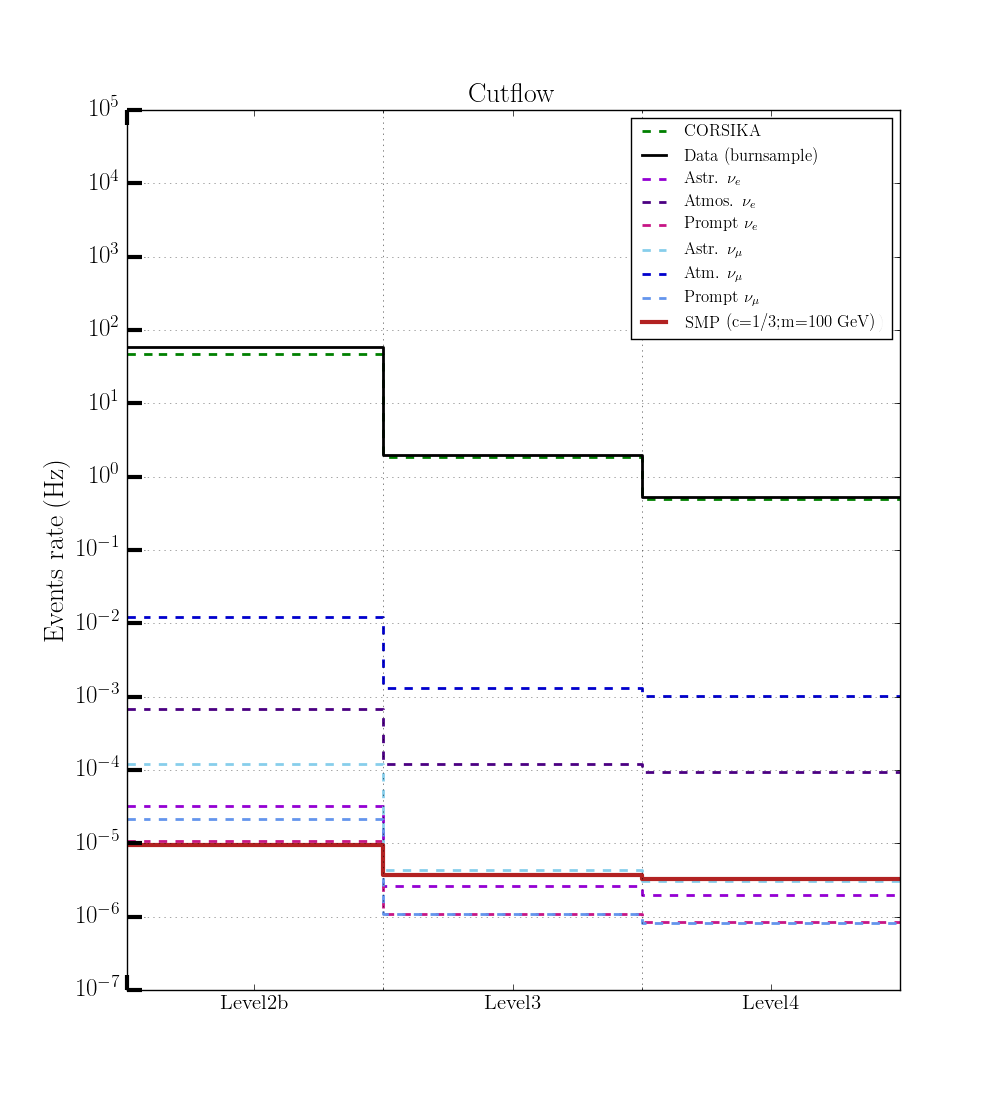
\includegraphics[width=0.8\textwidth]{chapter8/img/CutFlow_Level2b_Level3_Level4.png}
\caption{Event rate at three steps in the analysis. Data from the burn sample is shown in black, several Monte Carlo background samples are shown with dashed lines and the solid red line corresponds to one signal sample of an SMP with charge 1/3 and mass 100 GeV. ``CORSIKA'' corresponds to events from air shower simulations.}
\label{fig:cutflow}
\end{figure}


\section{Filter selection}
\label{sec:filterselection}
As explained in Section \ref{subsec:filters}, IceCube data is processed through multiple filters. Since this analysis is the first of its kind in the collaboration, the choice was to start from scratch and not use a processed dataset from another analysis\footnote{Since many searches look for similar signatures or deal with similar backgrounds, processed data sets in the collaboration are often used for multiple analyses.}. Therefore, a combination of filters was chosen that is able to distinguish signal events from background as best as possible at this preliminary stage. An illustration of filter combination efficiency is given in Figure \ref{fig:filterrate}. The efficiency is defined as the percentage of simulated particles that pass a certain filter. The figure shows many possible filter combinations and are ranked in function signal efficiency. The efficiency of the filter combination should be as high as possible for the signal, and as low as possible for background events. Therefore, the combination of four filters was chosen. This filter selection will be referred to as \textit{Level 2b} as an addition to filter processing in Level 2 (see Section \ref{sec:processing}). The filters that were included in this stage are the VEF, LowUp, Online Muon L2, and DeepCore filters. They are explained in more detail below. 

\begin{figure}
\centering
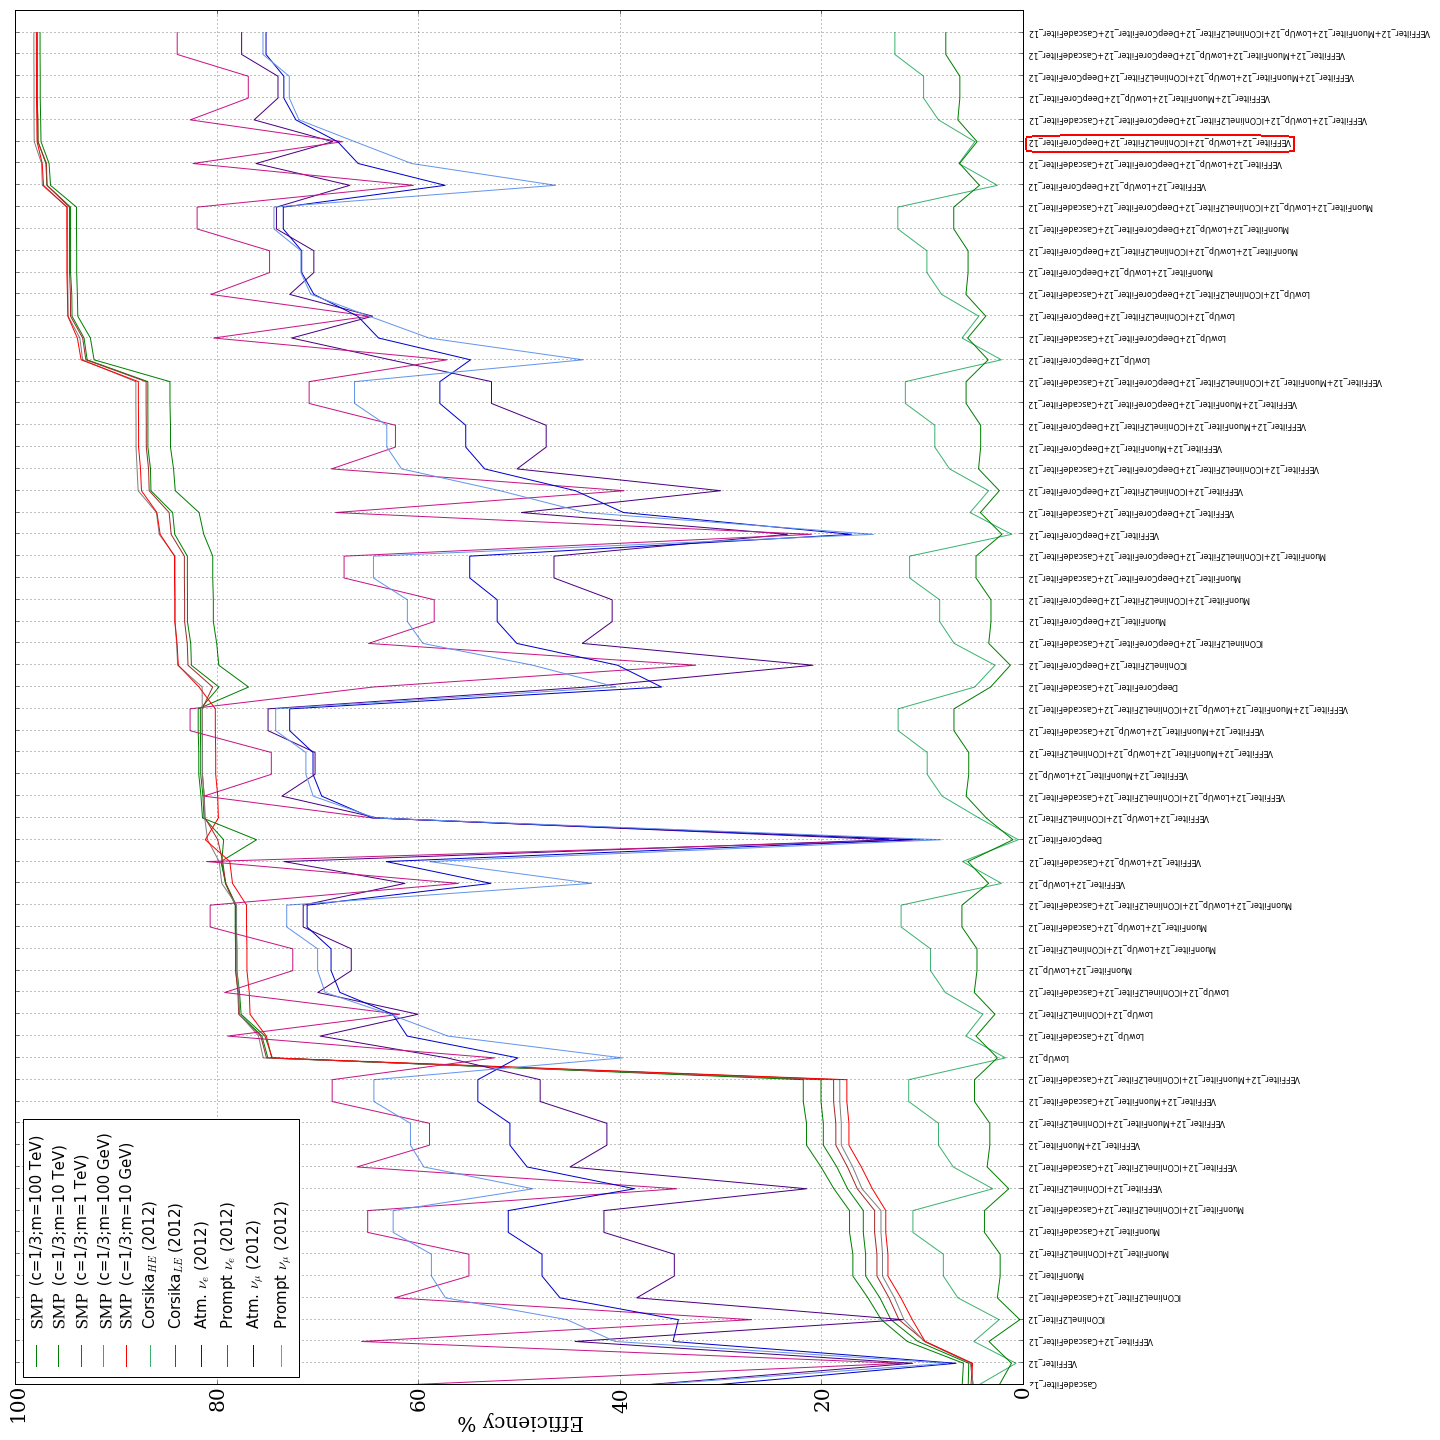
\includegraphics[width=\textwidth,height=0.85\textheight]{chapter8/img/FilterRate_better_rotated}
\caption{Illustration of the efficiencies of several filters and their possible combinations. The x-axis was determined by starting with filter selections that had a low efficiency in signal selection and ranges from low to high signal performance. Five signal points for a fixed charge and different mass show similar results. SMPs with charges 1/2 and 2/3 show similar results but are left out for a better visualization. An upgoing signal sample was used to determine the signal efficiency. The chosen filter combination is shown in red.}
\label{fig:filterrate}
\end{figure}

\subsection{VEF}
The Vertical Event Filter (VEF) is originally designed for oscillation and Earth WIMP analyses and makes use of the string trigger (see Section \ref{subsec:triggers}). An SMP that travels in a direction following a string, or close by, can trigger optical modules even though the total light yield of an event is low (other trigger hits are unlikely in this scenario), making this filter an ideal part of the filters that are selected. The filter ignores HLC hits in the top 5 DOM layers to reduce the muonic component from air shower events and other selection cuts try to further refine the search region, in particular for WIMP events (see Section \ref{subsubsec:DM}). For example, the \texttt{LineFit} zenith angle should be higher than 166.2$^\circ$, focussing on upgoing tracks. More information can be found in Ref. \cite{VEF2012}.

%meeste hiervan: https://docushare.icecube.wisc.edu/dsweb/Get/Document-62750/VEF_2013_proposal.pdf

\subsection{LowUp}
The primary motive for the LowUp filter design is again focussed on WIMP searches, but is also used in atmospheric neutrino analyses. It is set up to capture upgoing muons with an energy below 1 TeV. The majority of the events that are selected by this filter make use of the in-ice Volume Trigger, but also the in-ice SMT8, in-ice String and SMT3-DeepCore triggers are used for completeness (see Table \ref{tab:trigger}). The selection cuts are loose selections required to look for upgoing track-like particles. For example, the zenith angle of the reconstructed particle should be 80$^\circ$ or higher and the difference between the maximal $z$-coordinate and minimal $z$-coordinate of hit DOMs should be less than or equal to 600 m. More information can be found in Ref. \cite{LowUp2012}.

%je hebt een Nchan>=5 cut in je L4 zodat veranderingen in LowUp niet uitmaken :-)

\subsection{Online Muon L2}
The Online Muon L2 filter is a subset of the Muon Filter (see Ref. \cite{muon2012filter}) and tries to select the most interesting muon-like events while reducing the rate of the filter from around 30 Hz to 5 Hz, reducing the data stream by a factor of 6. Historically, this subset was data processed offline from the Muon Filter, but after realizing that this could be done online and because many analyses made use of this selection, it was chosen to implement it as a separate filter. The filter tries to select both upgoing and downgoing muons, with different selection cuts depending on the zenith angle of the particle reconstruction. The four selection ranges are defined as:
\vspace{2mm}
\begin{itemize}
\item $180^\circ \geq \theta_\textrm{MPE} \geq 115^\circ$ (upgoing)
\item $115^\circ > \theta_\textrm{MPE} \geq 82^\circ$ (upgoing)
\item $82^\circ > \theta_\textrm{MPE} \geq 66^\circ$ (downgoing)
\item $66^\circ > \theta_\textrm{MPE} \geq 0^\circ$ (downgoing)
\end{itemize}
\vspace{2mm}
where the particle reconstruction was done with MPE (Section \ref{subsec:spempe}), which was feasible if it only had to be done on the events passing the Muon Filter. The first two regions have an efficiency\footnote{Here defined as having a reconstruction within 3$^\circ$ of the MC truth.} higher than 99\%. The downgoing region requires additional cuts to remove the less interesting muons from air showers. The main variables used are the number of hit DOMs, likelihood parameters, number of PEs, etc. More information can be found in Ref. \cite{OnlineMuonL22012}.

\subsection{DeepCore}
A DeepCore specialized filter was added to account for SMP tracks that traverse the more densely instrumented DC detector. Due to the low amount of light produced by these dim tracks, adding the DeepCore filter (which is optimized for the DC instrumented volume) proved to be of significant importance.

The DeepCore filter was designed to look for very dim events coming from dark matter, low-energy neutrino oscillations, and for studies that are dedicated to observe atmospheric neutrinos below 100 GeV. The fiducial volume used for this filter consists of
\vspace{2mm}
\begin{itemize}
\item the bottom 22 DOMs on the IceCube strings 25, 26, 27, 34, 35, 36, 37, 44, 45, 46, 47 and 54;
\item the bottom 50 DOMs on the DeepCore strings 79-86.
\end{itemize}
\vspace{2mm}
These strings are indicated in Figure \ref{fig:deepcorestrings}.\\

\begin{figure}[t]
\centering
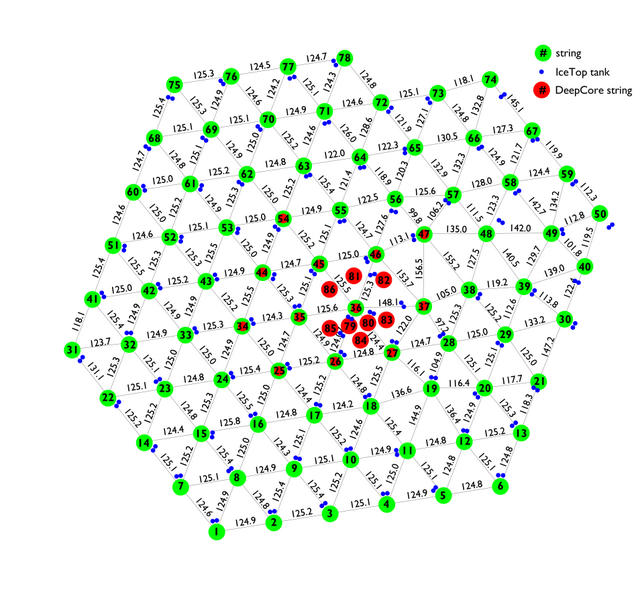
\includegraphics[width=0.55\textwidth]{chapter8/img/stringview.jpg}
\caption{Top view of the IceCube strings (and IceTop tanks) where the DeepCore fiducial volume is defined by the DeepCore strings (red) and several surrounding in-ice IceCube strings (green and red).}
\label{fig:deepcorestrings}
\end{figure}

\noindent The filter uses the DeepCore SMT3 trigger and additionally, two layers are used as a veto to remove events that probably originate from atmospheric muons. This is done by comparing the position and timing of all hits to the position and timing of several COGs that are constructed from these hits (see footnote pg. \pageref{footnote:cog} for the explanation of a COG). More information can be found in Ref. \cite{DeepCore2012}.

\subsection{Burn sample checks}
Before further processing, the burn sample (a subset of the data that is used to check if the Monte Carlo adequately describes the data) is compared over the different years that are used in the analysis. This is shown in Figure \ref{fig:burnsamplechecks}. The sine wave pattern from seasonal variations in the atmosphere (see Section \ref{subsub:corsika}) is clearly visible and consistent over the years. The $x$-axis is more spread out in the first years due to the larger amount of test runs. The shift in data rate in early 2011 runs is caused by a DOM software change that was introduced in the Summer of 2011 \cite{2011rate}. This phenomenon is well understood and since the changes are minimal, these runs are kept.
More information on the burn sample can be found in Section \ref{sec:burnsample}.

\begin{figure}[t]
\centering
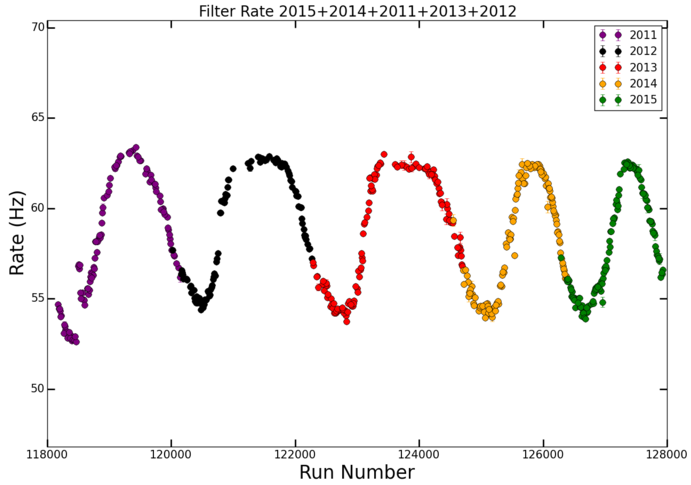
\includegraphics[width=0.49\textwidth]{chapter8/img/FilterRatePerRun.png}
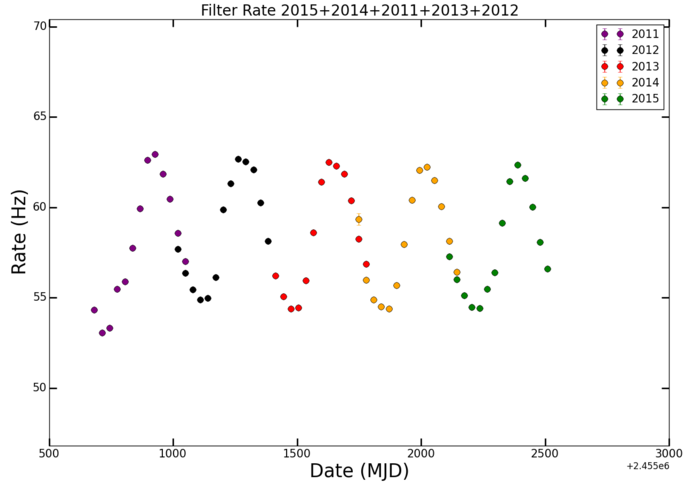
\includegraphics[width=0.49\textwidth]{chapter8/img/FilterRatePerMonth.png}
\caption{\textit{Left: }Total rate of the combined filters as a function of the run number. \textit{Right: }Total filter rate averaged per month. There is an overlap for each year because a new season does not necessarily start at the beginning of a month.}
\label{fig:burnsamplechecks}
\end{figure}

\section{Level 3}
The combined filter selection leads to a total rate of $\sim60$ Hz, or an expected $1.9$ billion events per year of livetime. The average event size at Level 2 is around 15 kB, which would result into around 30 TB of data per year of livetime.

Therefore, five quality cuts are implemented with a goal that is threefold:
\vspace{2mm}
\begin{enumerate}
\item Reduce the data rate,
\item Improve the signal to background ratio, increasing the selection purity,
\item Improve the agreement between data and Monte Carlo (as can be seen in Figure \ref{fig:cutflow}).
\end{enumerate}
\vspace{2mm}
\noindent These cuts are shown in Figures \ref{fig:level3cutszenith} to \ref{fig:level3stopping} and explained below.


\subsection{The zenith angle cut}
\label{subsec:zenithanglecut}
Even though there are no upgoing muons from air showers expected, the vast majority of events that pass the filter selections still originate from muons that are mis-reconstructed. Even though there is only a small chance of these events to have a reconstructed zenith angle with a large offset from the true angle, the expected flux of air showers is so much larger compared to the assumed signal flux that it still dominates by orders of magnitude. Therefore, a zenith angle cut was set at an angle of 

\begin{equation}
\theta_\textrm{zen} (\textrm{MPE}) \geq 85^\circ,
\end{equation}

\noindent where the cut is slightly relaxed to include events coming from the horizon. Muons passing through kilometers of air and ice have a much lower chance of reaching the detector.\\

\noindent The zenith angle distribution of the MPE reconstruction can be seen in Figure \ref{fig:level3cutszenith}. Several background samples are shown in filled histograms. These samples are stacked together, where the largest samples are added last. The total rate of these Monte Carlo data samples corresponds to the top of these stacked histograms. Events from air showers are referred to as Corsika in the figures. The total statistical uncertainty of the background is indicated with a hatched grey color band. The burn sample is shown with black data points. The error bars correspond to the statistical uncertainty. The simulated signal samples are illustrated with a solid line.

Signal and background Monte Carlo samples are normalized to the livetime of the burn sample.

The upwards trend to higher zenith angles of several samples is due to the filter selections that depend on the angle. 

\begin{figure}[t]
\centering
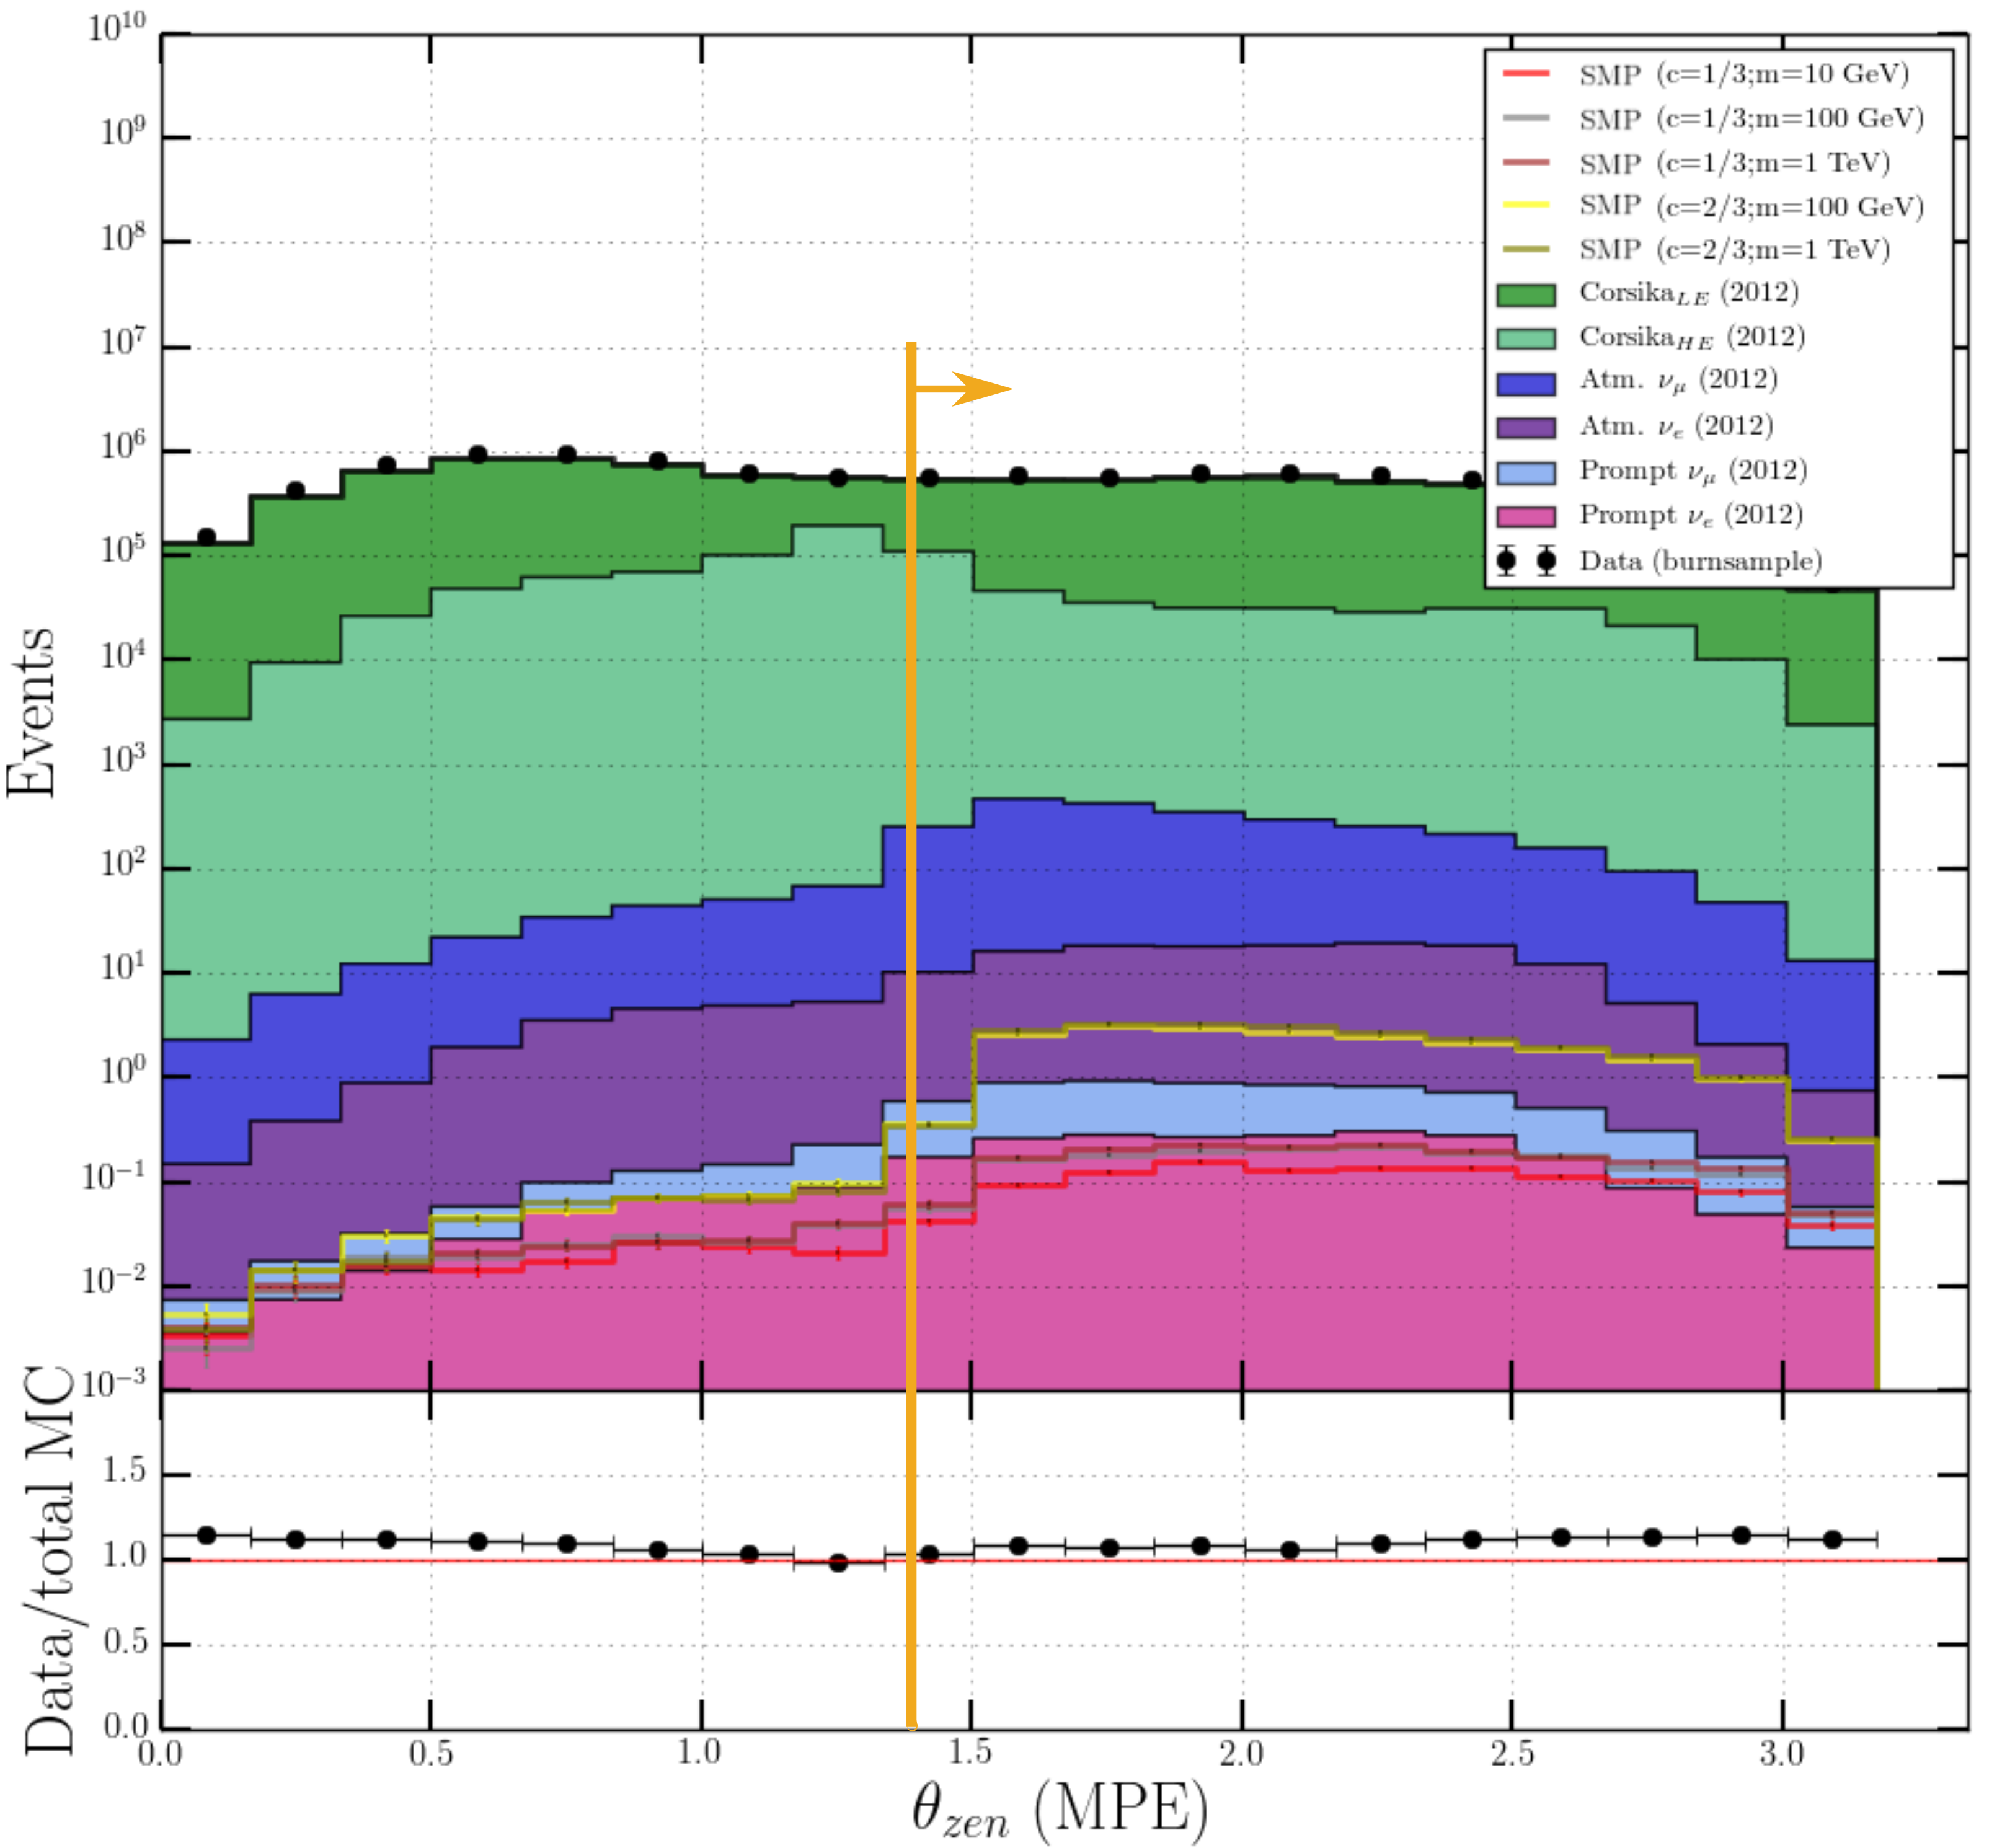
\includegraphics[width=0.7\textwidth]{chapter8/img/1D_stack_mpefit_zenith_new.png}
\caption{Number of events as a function of the MPE reconstructed zenith angle and normalized to the burn sample. The cut is illustrated with an orange line, the arrow points towards the events that are kept.}
\label{fig:level3cutszenith}
\end{figure}


\subsection{The rlogL cut}
The reduced log-likelihood, rlogL, of the track reconstruction fit is used as a goodness-of-fit variable. The term ``reduced'' is used because the logarithm of the likelihood is normalized by the number of degrees of freedom (NDOF) in the track fit

\begin{equation}
\textrm{rlogL} = \frac{\log \mathcal{L}}{\textrm{NDOF}} = \frac{\log \mathcal{L}}{\textrm{NCh} - \textrm{NPara}},
\end{equation}
where NCh is the number of channels/DOMs and NPara the number of fitted parameters (3 for the position and 2 for the track direction). For Gaussian probability distributions this expression corresponds to the reduced chi-square. Lower values indicate better reconstructions\footnote{Here, the $-\log \mathcal{L}$ is used.}, therefore the rlogL cut was set at a value of 

\begin{equation}
\textrm{rlogL} < 15.
\end{equation}

The rlogL distribution can be seen in Figure \ref{fig:level3cutsrlogl}. Data and Monte Carlo disagree at larger values due to non-perfect simulations. Events that lead to bad reconstructions are not, or not well, simulated and are removed with this cut.


\begin{figure}[t]
\centering
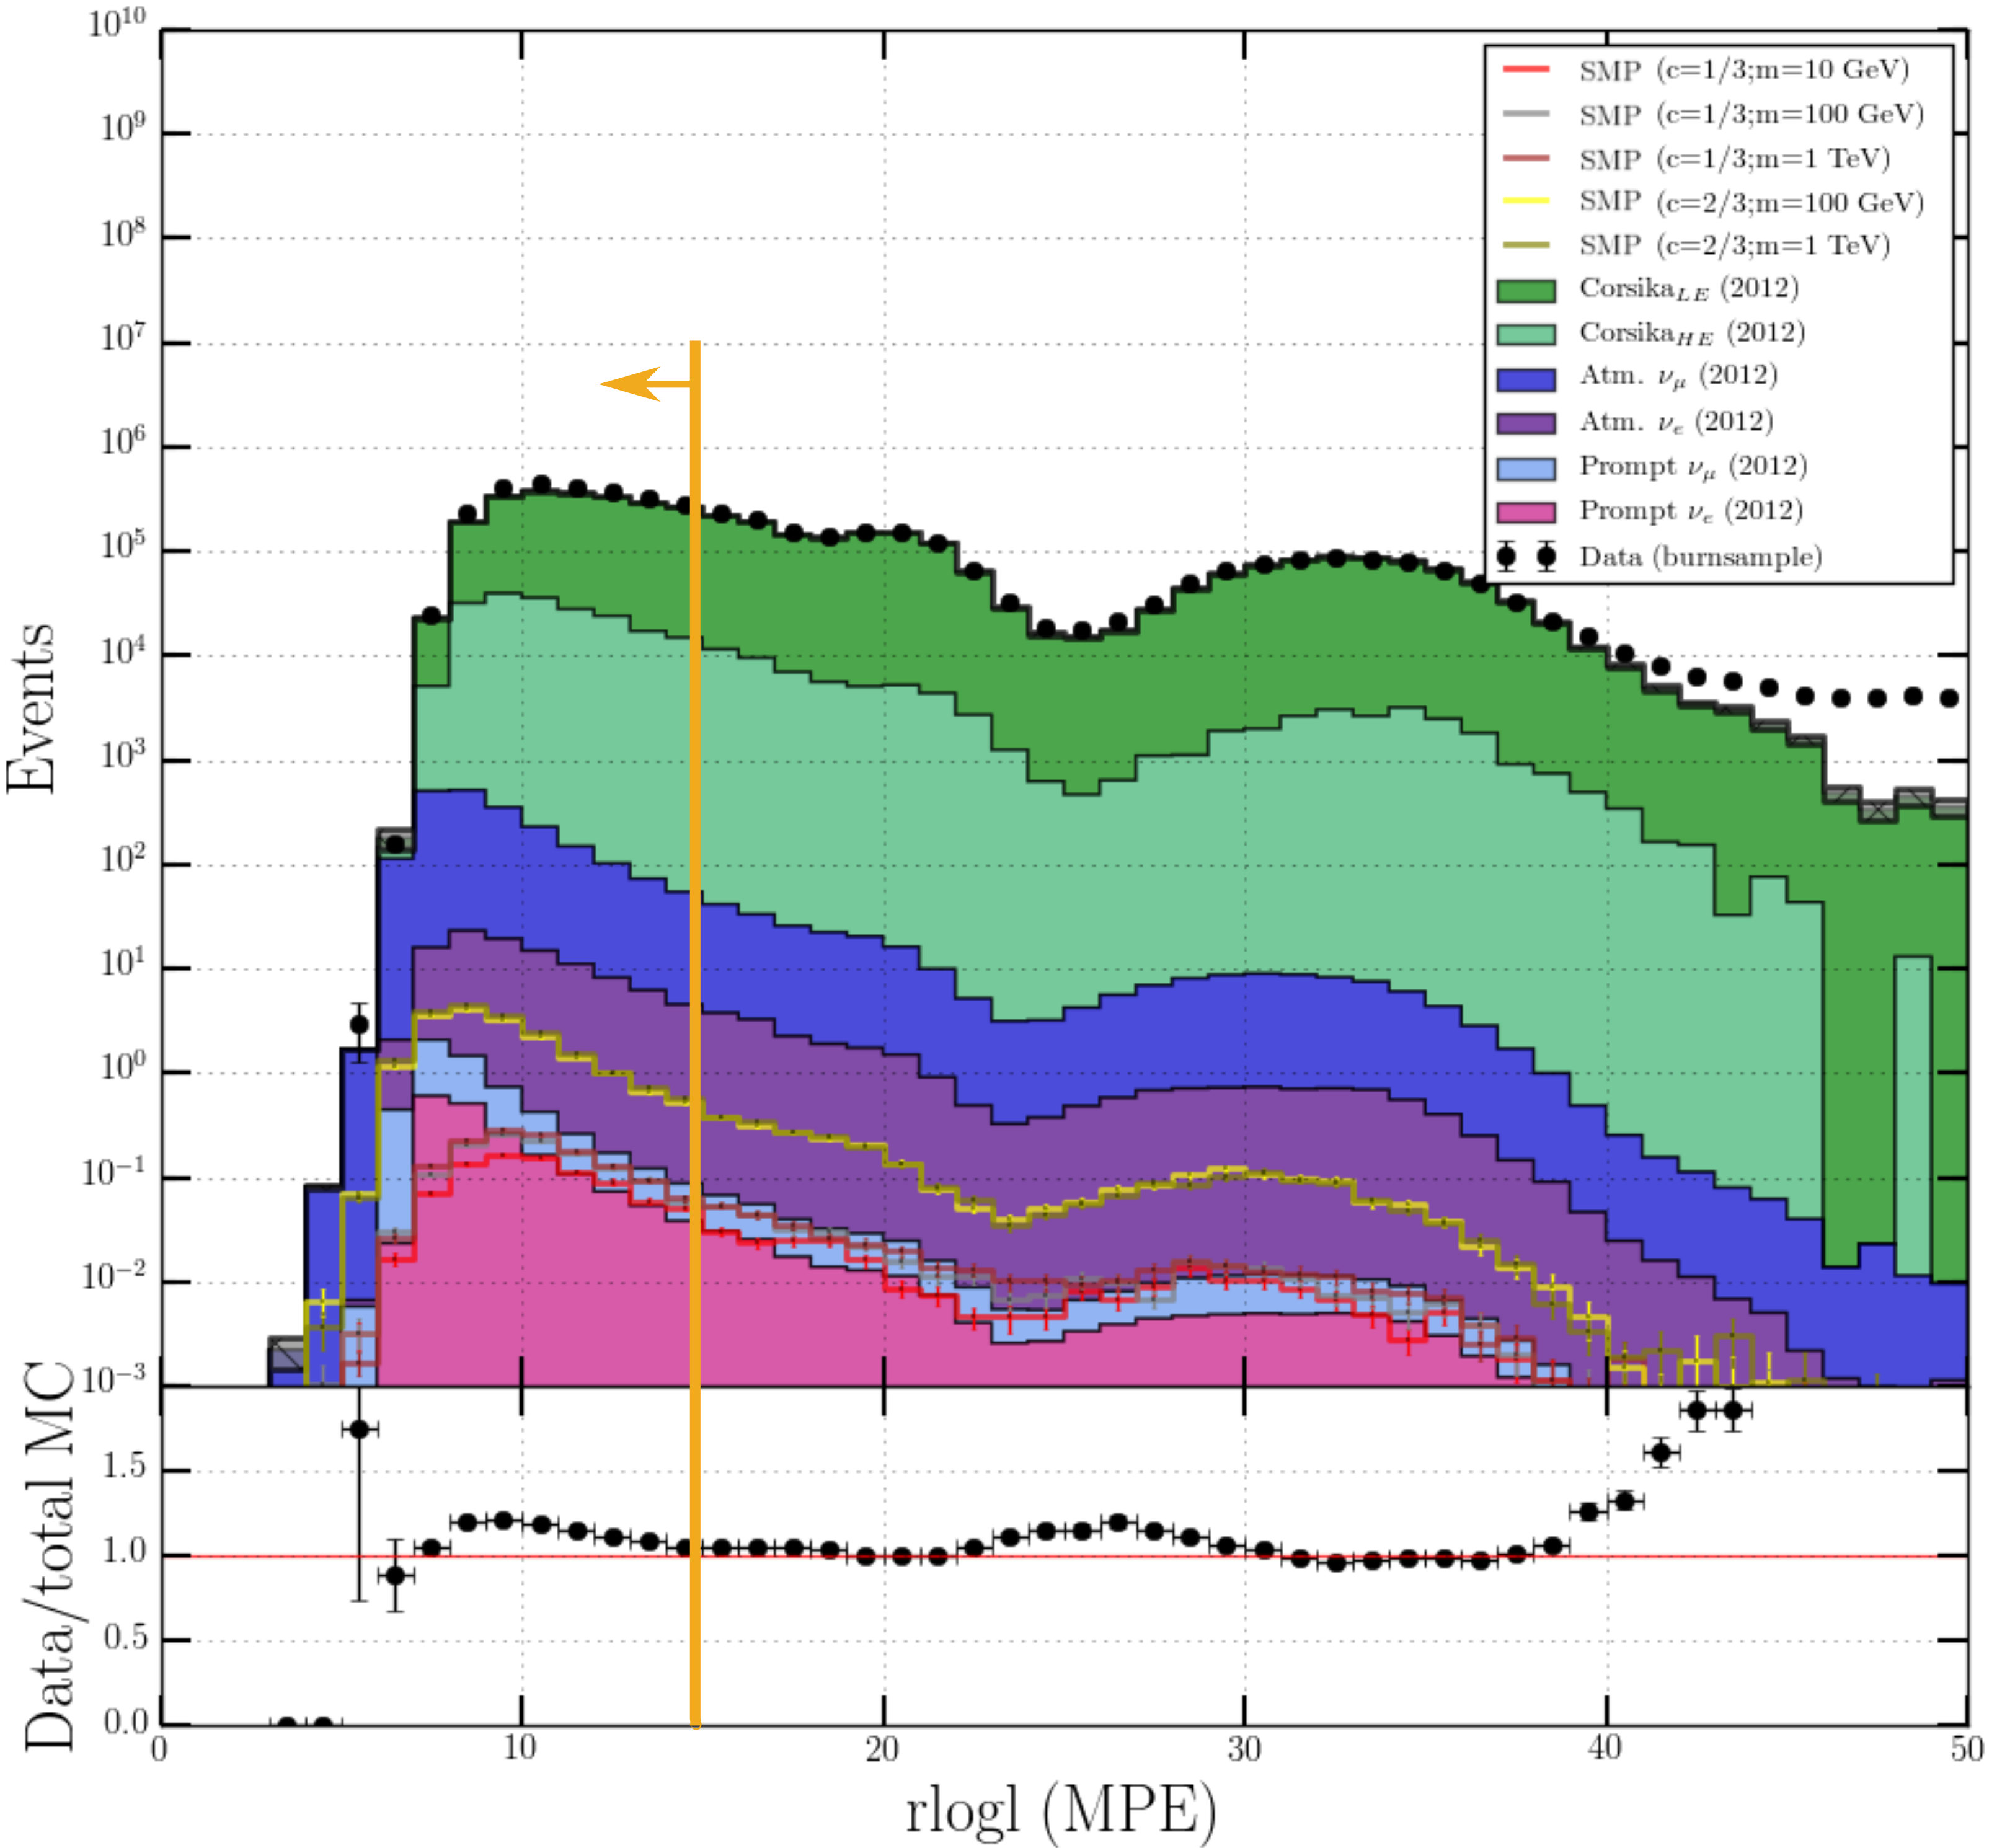
\includegraphics[width=0.7\textwidth]{chapter8/img/1D_stack_mpefit_rlogl_new.png}
\caption{Number of events as a function of rlogL normalized to the burn sample. The cut is illustrated with an orange line, the arrow points towards the events that are kept.}
\label{fig:level3cutsrlogl}
\end{figure}


\subsection{The NPE cut}
The total number of photoelectrons seen in the detector for an event is correlated to the number of photons that were emitted from the track. The Frank-Tamm formula in Eq. \ref{eq:franktamm} shows that that particles with a charge $< 1$ will produce less Cherenkov light. Therefore a cut on the total number of photoelectrons was set at a value of 

\begin{equation}
\textrm{NPE} < 50.
\end{equation} 

The NPE distribution can be seen in Figure \ref{fig:level3npe}. Signal samples with a lower charge clearly show NPE distributions that peak at lower values, as  expected. 

\begin{figure}[t]
\centering
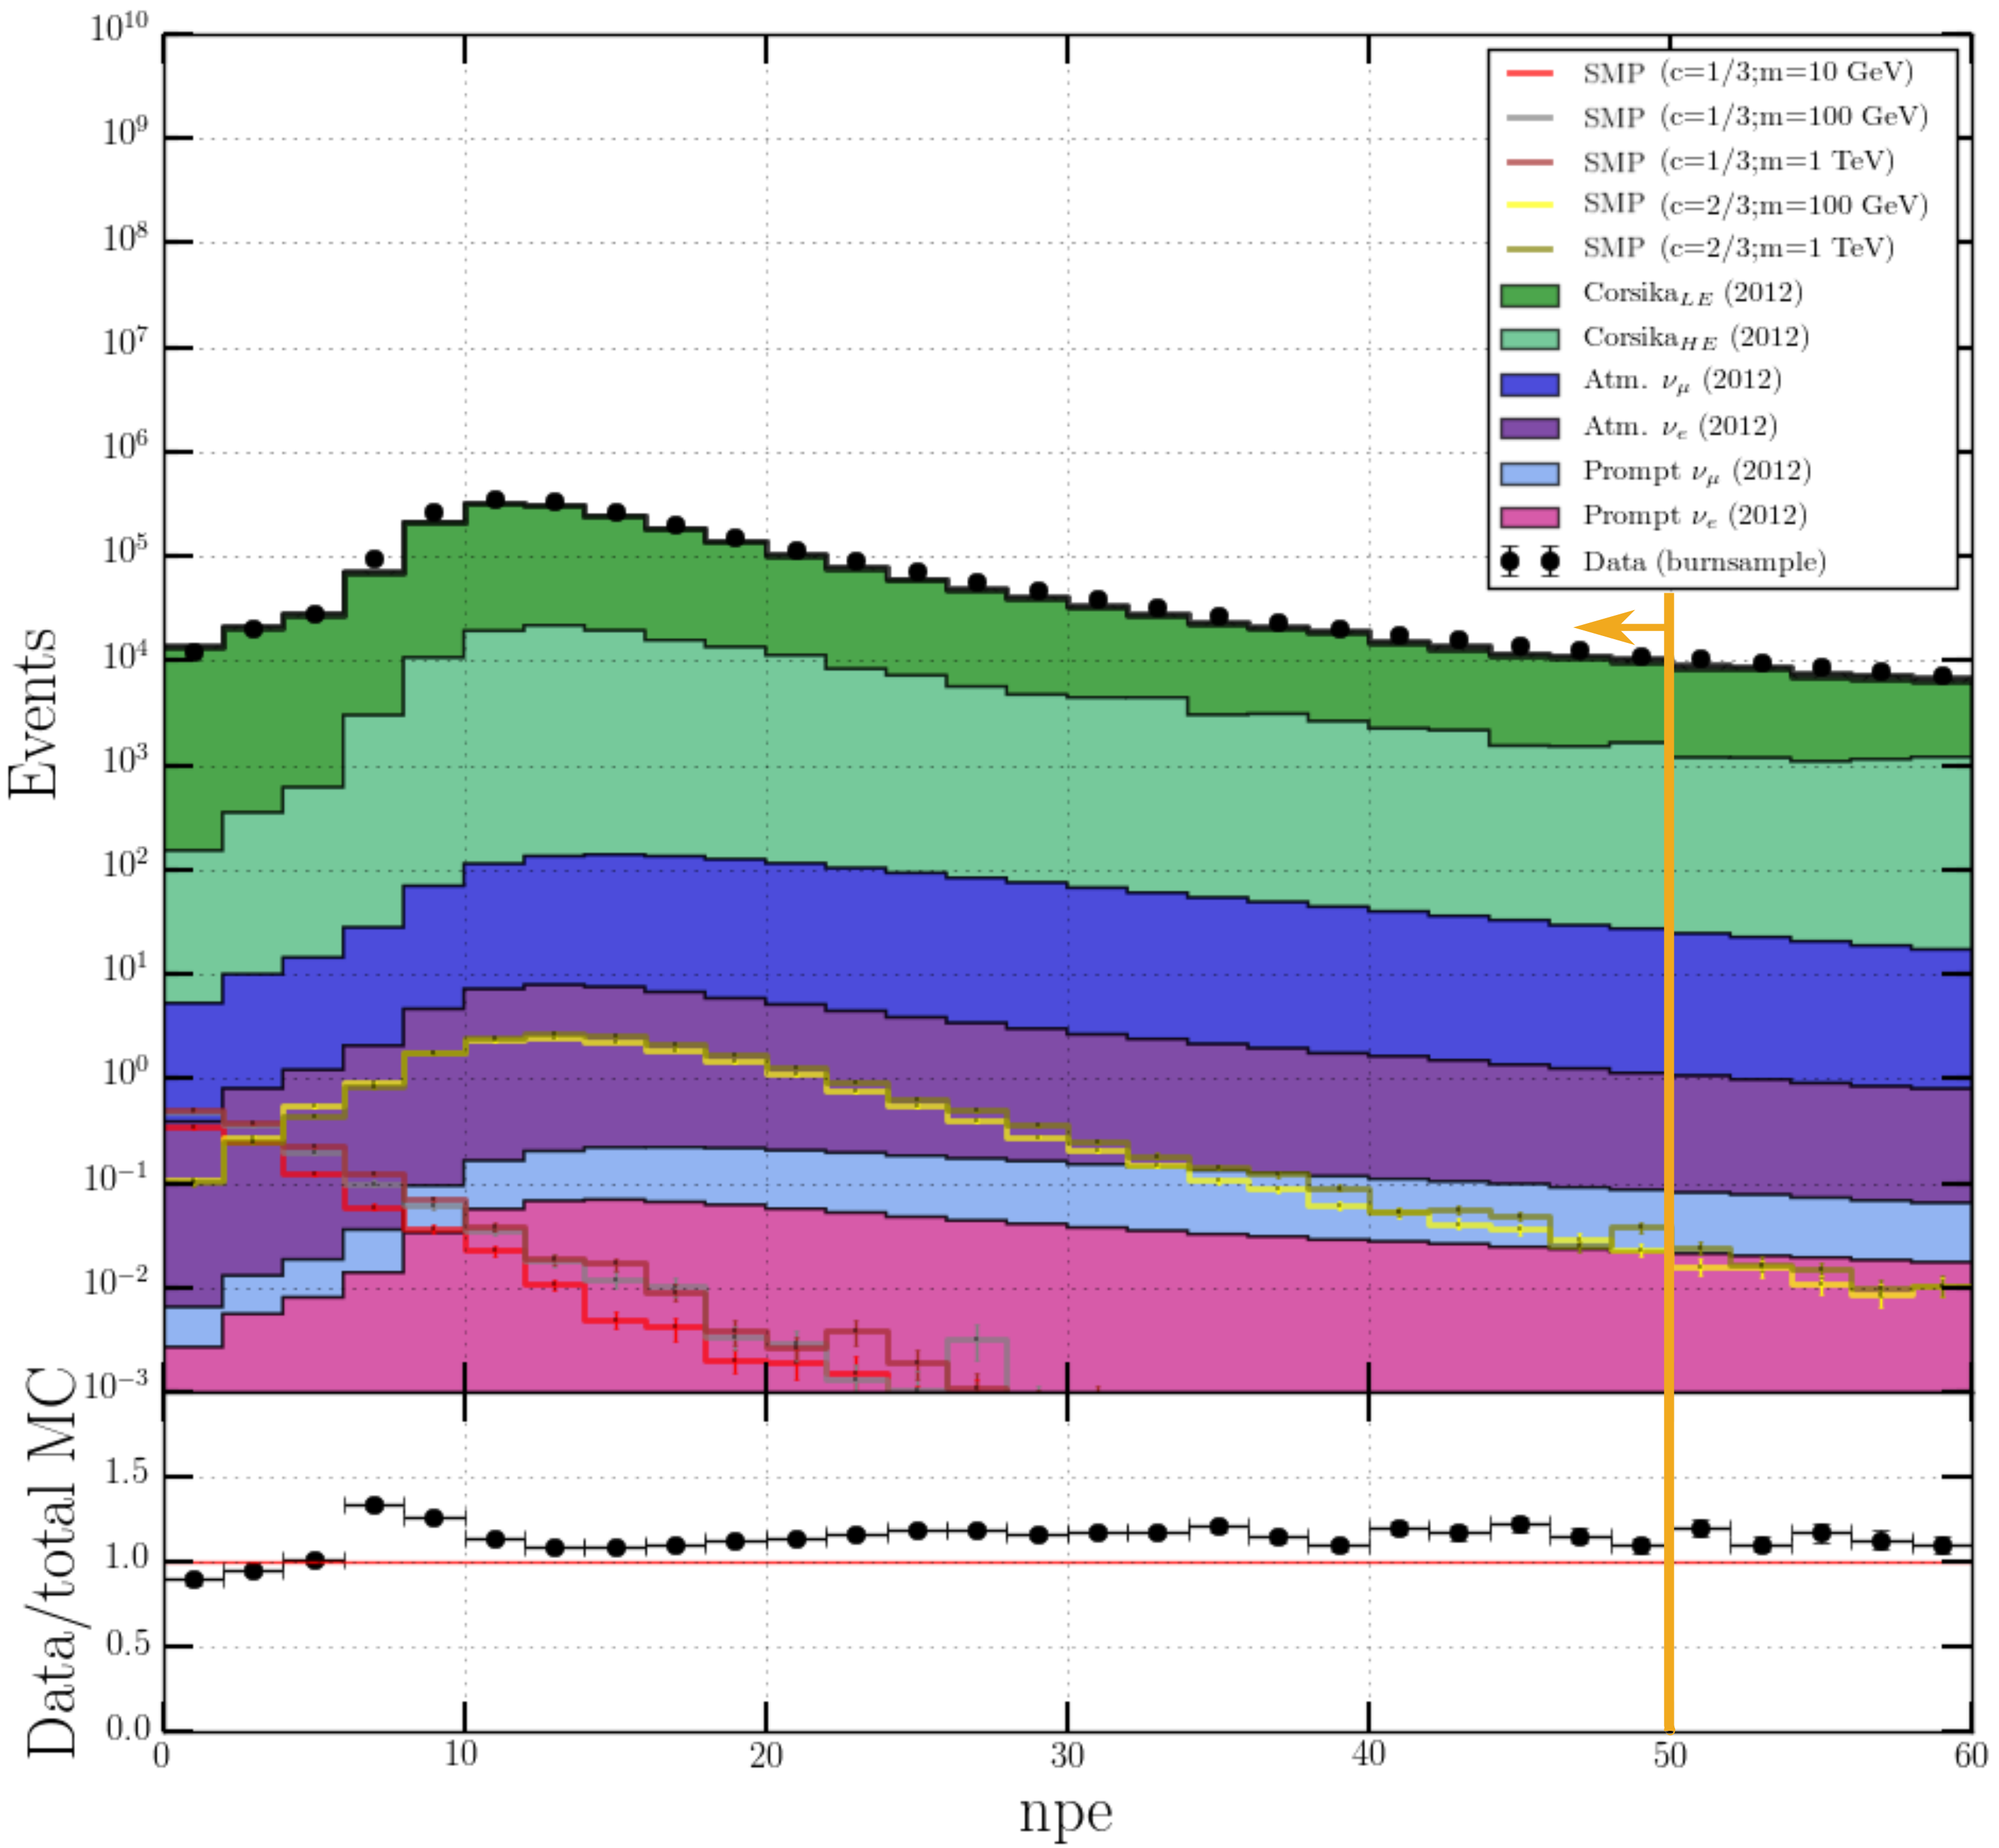
\includegraphics[width=0.7\textwidth]{chapter8/img/L3_zenithcut_gr_1p4835298642_rloglcut_less_15_1D_stack_npe_new.png}
\caption{Number of events as a function of number of photoelectrons (NPE) seen in the detector. The cut is illustrated with an orange line, the arrow points towards the events that are kept.}
\label{fig:level3npe}
\end{figure}

\subsection{The starting rlogL cut}
The relative probability for tracks to be starting and/or stopping can be estimated with the \texttt{FiniteReco} module (see Section \ref{subsec:finitereco}). Because many low-energetic muons would be starting and/or stopping in the detector, these likelihoods prove to be a powerful tool in removing these events. High-energetic muons will have a higher chance of being throughgoing, but would produce much more light than the dim tracks that are expected for the SMPs. These are mostly removed with the NPE cut.

The likelihood is always compared to the likelihood of throughgoing tracks, hence the ``relative probability''. It was chosen to place the starting relative logL at a value of 

\begin{equation}
\textrm{rel\_logL}(\textrm{starting}) = \textrm{logL}(\textrm{starting}) - \textrm{logL}(\textrm{throughgoing}) > 0. 
\end{equation}

The starting rlogL distribution can be seen in Figure \ref{fig:level3starting}. Because the log-likelihoods are negative, positive number indicate larger probabilities for throughgoing tracks. We can see that there is a large contribution of starting tracks in the background due to the filter requirements and previous cuts that focus on dim tracks.

\begin{figure}[t]
\centering
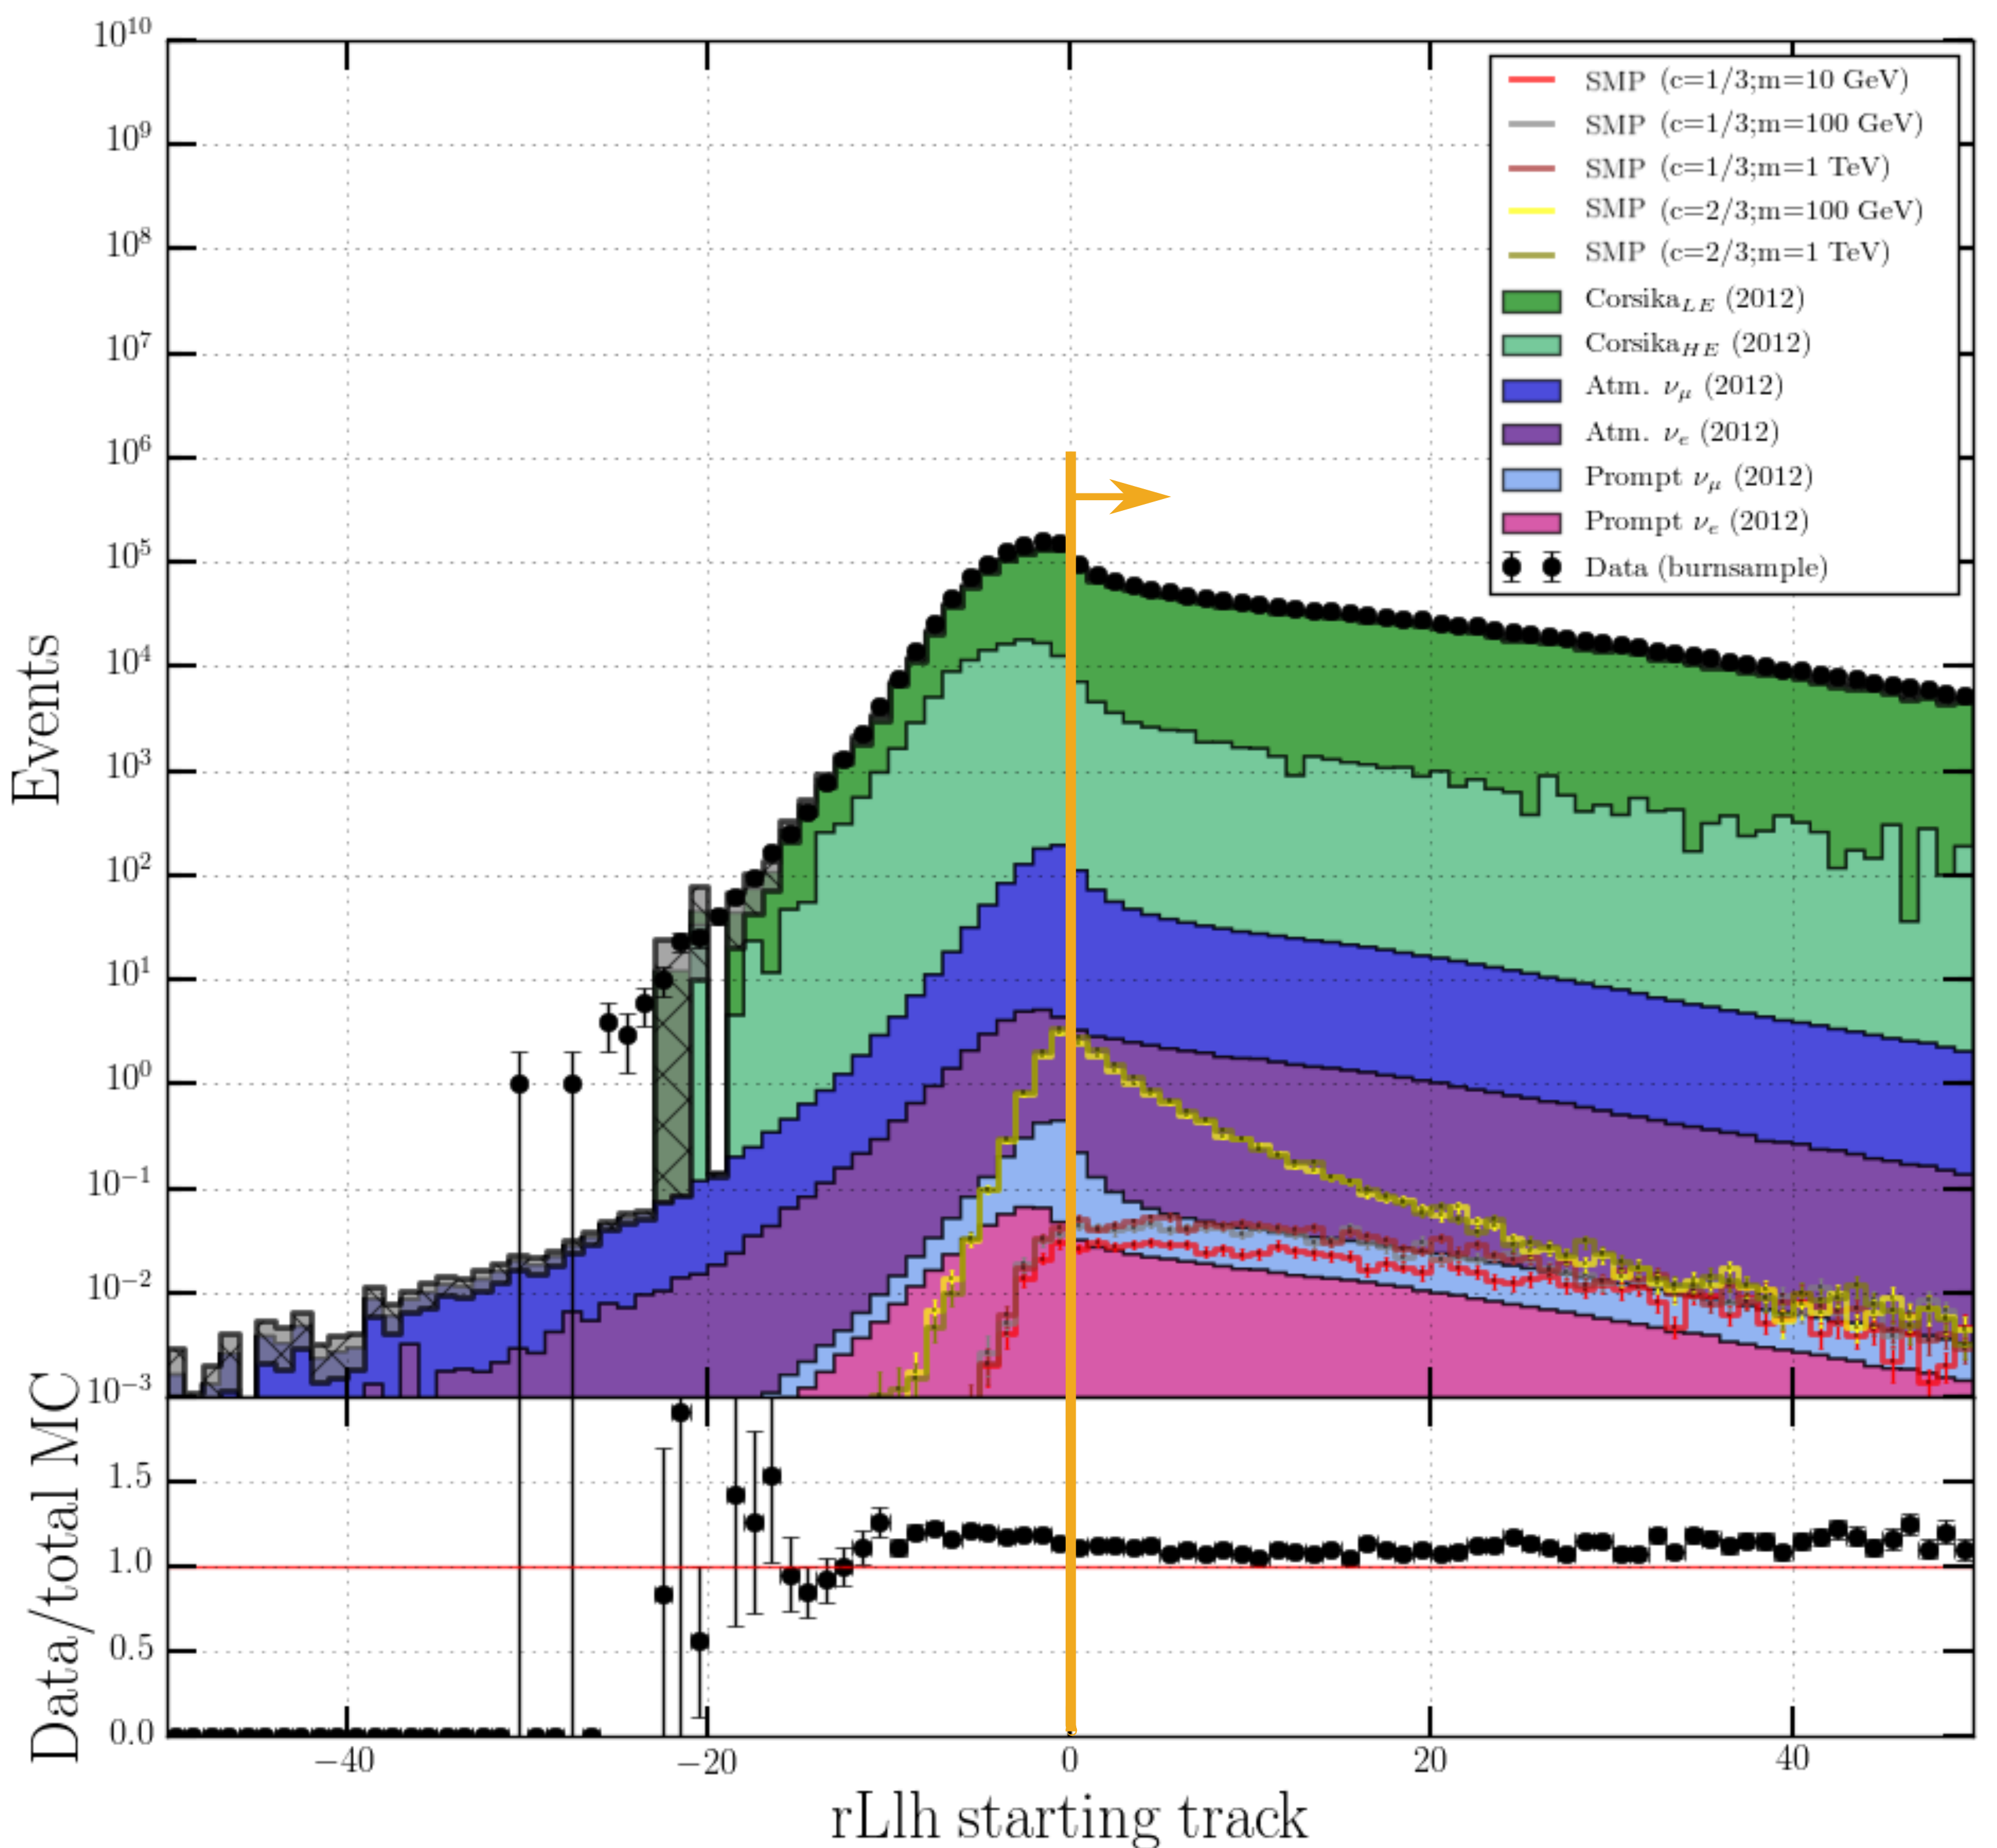
\includegraphics[width=0.7\textwidth]{chapter8/img/L3_zenithcut_gr_1p4835298642_rloglcut_less_15_npecut_less_50_1D_stack_finitereco_rllh_starting_new.png}
\caption{Number of events as a function of the starting likelihood. The cut is illustrated with an orange line, the arrow points towards the events that are kept.}
\label{fig:level3starting}
\end{figure}

\subsection{The stopping rlogL cut}
Analogous to the previous cut, it was chosen to place the stopping relative logL at a value of
\begin{equation}
\textrm{rel\_logL}(\textrm{stopping}) = \textrm{logL}(\textrm{stopping}) - \textrm{logL}(\textrm{throughgoing}) > 10. 
\end{equation}

The stopping rlogL distribution can be seen in Figure \ref{fig:level3stopping}. Because the log-likelihoods are negative, positive number indicate larger probabilities for throughgoing tracks. We can see that there is a large contribution of stopping tracks in the background due to the filter requirements and previous cuts that focus on dim tracks.

\begin{figure}[t]
\centering
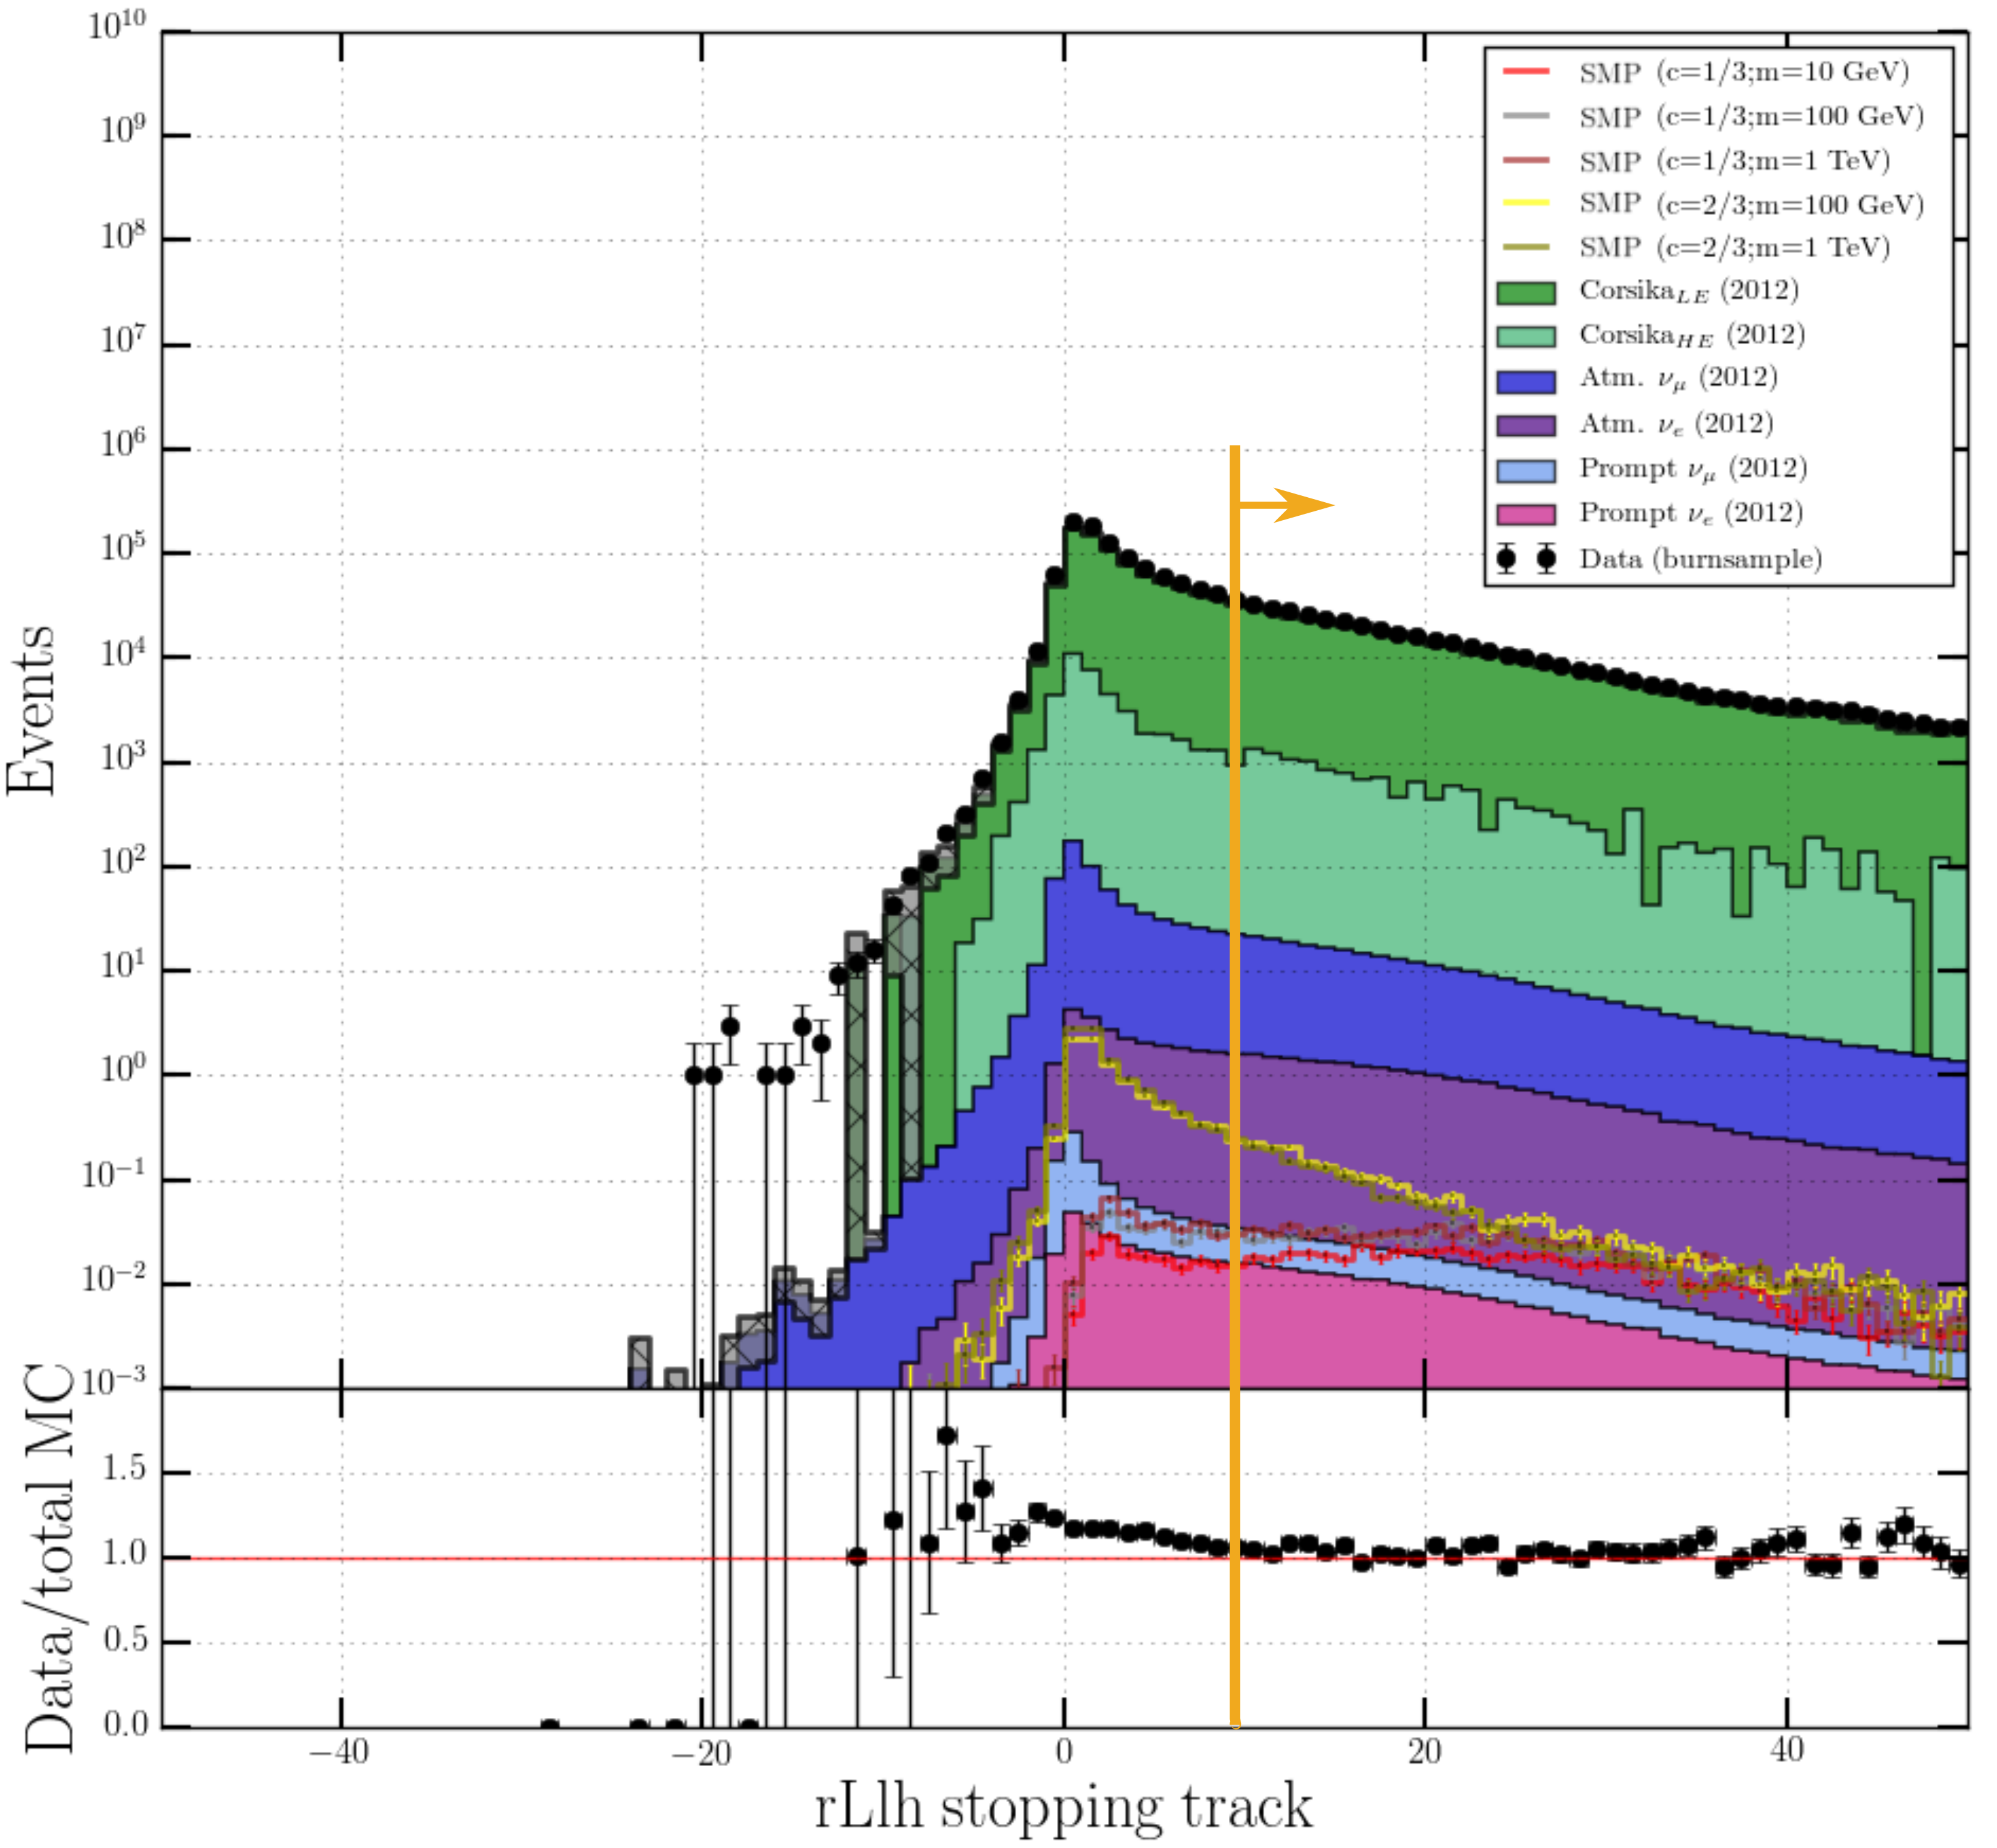
\includegraphics[width=0.7\textwidth]{chapter8/img/L3_zenithcut_gr_1p4835298642_rloglcut_less_15_npecut_less_50_startingtrackcut_hs_gr_0_1D_stack_finitereco_rllh_stopping_new.png}
\caption{Number of events as a function of the stopping likelihood. The cut is illustrated with an orange line, the arrow points towards the events that are kept.}
\label{fig:level3stopping}
\end{figure}

\section{Level 4}
As can be seen in Figure \ref{fig:level3stopping}, most of the background at this point in the analysis still originates from air showers. However, due to the Level 3 quality cuts, the total rate was reduced from around $\sim 60$ Hz to $\sim2$ Hz (as can be seen in Figure \ref{fig:cutflow}), low enough for more elaborate variables to be computed and more aggressive cleaning. In Level 4, the IceHive splitting and cleaning tools (see Section \ref{sec:icehive}) were implemented and particle reconstructions on these ``new'' events were run again. Additional quality cuts were added to this level to ensure higher quality events. An overview is given in Table \ref{tab:level4}. Finally, new variables were constructed that will be used in Level 5.

\begin{table}[]
\caption{Overview of quality cuts in Level 4.}
\label{tab:level4}
\resizebox{\textwidth}{!}{%
\begin{tabular}{|l |c|c|c|}
\hline
\cellcolor[HTML]{F1A91E}Variable & \cellcolor[HTML]{F1A91E}Definition & \cellcolor[HTML]{F1A91E}Cut & \cellcolor[HTML]{F1A91E}Motivation \\ \hline
\textbf{nCh} & Number of hit DOMs & $\geq 5$ & Allows for better reconstructions \\ \hline
\textbf{nStr} & Number of hit strings & $\geq 2$ & Allows for better reconstructions \\ \hline
\textbf{nStr\_in} & \begin{tabular}[c]{@{}c@{}}The number of hit inner strings.\\ An inner string is not located at the edge of the detector\end{tabular} & $\geq 1$ & Reduce leak-in events \\ \hline
\textbf{Fitstatus MPE} & Status of MPE reconstruction & Status == 'OK' & Remove bad reconstructions \\ \hline
$\mathbf{\theta_{HC}}$ \textbf{(MPE)} & Zenith angle cut on HiveCleaned pulses & $\geq 85^\circ$ & \begin{tabular}[c]{@{}c@{}}Similar to cut explained in Section \ref{subsec:zenithanglecut}:\\ focus on upgoing tracks\end{tabular} \\ \hline
\textbf{Innerstring domination} & See text inline & == True & See text inline \\ \hline
\end{tabular}%
}
\end{table}

\subsection{Cleaning and quality cuts}
\noindent IceHive provides a thorough cleaning method, sometimes resulting into events with a very low amount of hit DOMs. However, a minimal amount of hits is required to have reasonable and trustworthy particle reconstructions. Similarly, more than one string should have a hit to allow for better reconstructions due to the sparse distribution of the strings in the detector. Therefore, there are requirements on the minimum amount of DOMs and strings that should be hit as can be seen in Table \ref{tab:level4}. Because light is able to reach the edge of the detector even if the closest approach of very bright events is tens or hundreds of meters away, it would be near impossible to distinguish bright events far from the detector from dim tracks passing closeby. Therefore, it was required that at least one string that is not on the edge of the detector should have hit DOMs to reduce these \textit{leak-in events}.
The zenith angle cut is re-introduced on the new event that should have better reconstructions due to cleaning and finally, there is a requirement for ``innerstring domination''.

\paragraph{Innerstring domination}
Several types of events at the boundary of the detector can be a problem for an upgoing track analysis. This includes event classes such as:

\vspace{2mm}
\begin{itemize}
\item (Leak-in) Events from particles that are heading towards the instrumented volume, but stop right before they reach it or pass close by the detector. These ``leak'' light to the detector boundaries.
\item (Boundary) Events from particles that partially penetrate the detector on the boundary lines and possibly have a cascade at the endpoint. These events have rather cascade-like characteristics.
\item (Corner-clippers) Events from particles that are throughgoing on the corners of the detector and therefore have a COG at a corner of the detector\footnote{Two coincident corner-clippers could be a large nuisance in this analysis.}.
\item (Leak-out) Events originating from a neutrino that passes through almost the entire length of the detector and only has an interaction vertex right before leaving the detector. Depending on position and angle, the reverse direction of reconstruction can be of similar probability and thus a nuisance.
\end{itemize}
\vspace{2mm}

\noindent All these event classes have a high uncertainty in the reconstruction or even fail the reconstruction completely. Most of these events are removed with the requirement of an ``innerstring domination''.

DOMs are defined as outer DOMs if they are one of the following:

\vspace{2mm}
\begin{itemize}
\item part of a string on the edge of the detector,
\item on the bottom of strings 1-78,
\item on the top of strings 1-78.
\end{itemize}
\vspace{2mm}

\noindent The innerstring domination is set to \texttt{True} when 

\begin{equation}
\frac{\# \textrm{outer DOMs}}{\#\textrm{inner DOMs}} < 0.5,
\end{equation}
\noindent and set to \texttt{False} otherwise.

\subsection{Variable construction}
To distinguish signal from background events, variables that show a clear difference in their distribution have the most discriminative power. Therefore, in this part of the analysis, several new variables are introduced with this goal. Some variables used in Level 5 are already explained in Chapter \ref{ch:reconstruction} and are briefly mentioned in Section \ref{subsub:other}. A summary of all the variables that are constructed in Level 4 is given in Table \ref{tab:mrmrimportance}.

\subsubsection{Commonvariables}
\label{subsub:commonvariables}
Many analyses in the collaboration characterize certain parameters of an event in a similar fashion. However, some of these parameters were constructed slightly different, making them a cause of errors\footnote{For example: how is the length of a track defined? Is it the distance between the two furthest hits? Or the length between the first and the last hit? Or is it the distance between two COGs?}. Multiple variables were therefore combined into one project, called ``Commonvariables''. The variables used here can be subdivided into three categories: track characteristics, hit statistics, and time characteristics and are summarized and explained in Table \ref{tab:commonvariables}. Their distributions are shown in Figures. \ref{fig:commonvariablesavgdistdom150} to \ref{fig:commonvariableszpattern}.

Because DeepCore (DC) and IceCube (IC) DOMs have different quantum efficiencies (see Section \ref{subsec:DC}), the pulses from DC and IC DOMs should not be mixed for an unambiguous definition. Therefore either only DC or IC pulses are used to compute these variables depending if an event is \textit{IC dominated} or \textit{DC dominated}, where the former is set at $\frac{\# \textrm{DOMs}_\textrm{IC}}{\# \textrm{DOMs}_\textrm{DC}} \geq 0.5$ and the latter otherwise.\\

\noindent The variables used in this analysis are listed below.

\begin{table}[]
\centering
\caption{List of Commonvariables used in this analysis.} 
%\vspace{2mm}
\label{tab:commonvariables}
\resizebox{\textwidth}{!}{%
\begin{tabular}{|l |c|c|}
\hline
\cellcolor[HTML]{F1A91E}Category & \cellcolor[HTML]{F1A91E}Variable & \cellcolor[HTML]{F1A91E}Description \\ \hline
& AvgDistToDom & \begin{tabular}[c]{@{}c@{}}The average distance of the DOMs to the reconstructed track, \\ weighted by the total charge of each DOM.\end{tabular} \\ \cline{2-3} 
& EmptyHits & \begin{tabular}[c]{@{}c@{}}The maximal track length along the reconstructed track that \\ got no hits within a cylinder around the track.\end{tabular} \\ \cline{2-3} 
& \begin{tabular}[c]{@{}c@{}} TrackSeparation/\\COG Separation\end{tabular} & \begin{tabular}[c]{@{}c@{}}Distance how far the COG positions of the first and the \\ last quartile of the hits are separated from each other.\end{tabular} \\ \cline{2-3} 
%\multirow{-4}{*}{\cellcolor[HTML]{F1A91E}\begin{tabular}[c]{@{}l@{}}  \end{tabular}
\multirow{-6}{*}{\begin{tabular}[c]{@{}l@{}}\textbf{Track} \\ \textbf{Characteristics}$^\dagger$\end{tabular}} & TrackDistribution & \begin{tabular}[c]{@{}c@{}}The track hits distribution smoothness value {[}-1;1{]} \\ shows how smooth the hits of the given pulse series\\ within the specified track cylinder radius are distributed \\ along the track.\end{tabular} \\ \hline
& ZTravel & \begin{tabular}[c]{@{}c@{}}ZTravel is the average difference of the $z$ value of all hit DOMs\\ with the first (in time) quartile $z$ value.\end{tabular} \\ \cline{2-3} 
\multirow{-3}{*}{\begin{tabular}[c]{@{}l@{}}\textbf{Hit} \\ \textbf{Statistics}\end{tabular}}  & ZMax & The maximum $z$ coordinate of all hit DOMs. \\ \hline
\begin{tabular}[c]{@{}l@{}}\textbf{Time}\\ \textbf{Characteristics}\end{tabular} & ZPattern & \begin{tabular}[c]{@{}c@{}}All first pulses per DOM are ordered in time. If a DOM\\ position of a pulse is higher than the previous pulse's DOM position, ZPattern\\ is increased with +1. If the DOM position is located lower \\ in the detector, ZPattern decreases with -1. \\ In general, this variable gives a tendency of the direction of a track.\end{tabular} \\ \hline
\end{tabular}%
}
\begin{flushleft}
\begin{footnotesize}
$^\dagger$ Whenever one of the track characteristics variables is shown/mentioned, the suffix (e.g. ``\_50'') refers to the track cylinder that was used around the track.
\end{footnotesize}
\end{flushleft}
\end{table}

\paragraph{AvgDistToDom}
Large values indicate bright tracks or events with many noise hits far away from the reconstructed track (seed track). Therefore, signal events peak at lower values than the backgrounds. This is shown in Figure \ref{fig:commonvariablesavgdistdom150}.

\begin{figure}
\centering
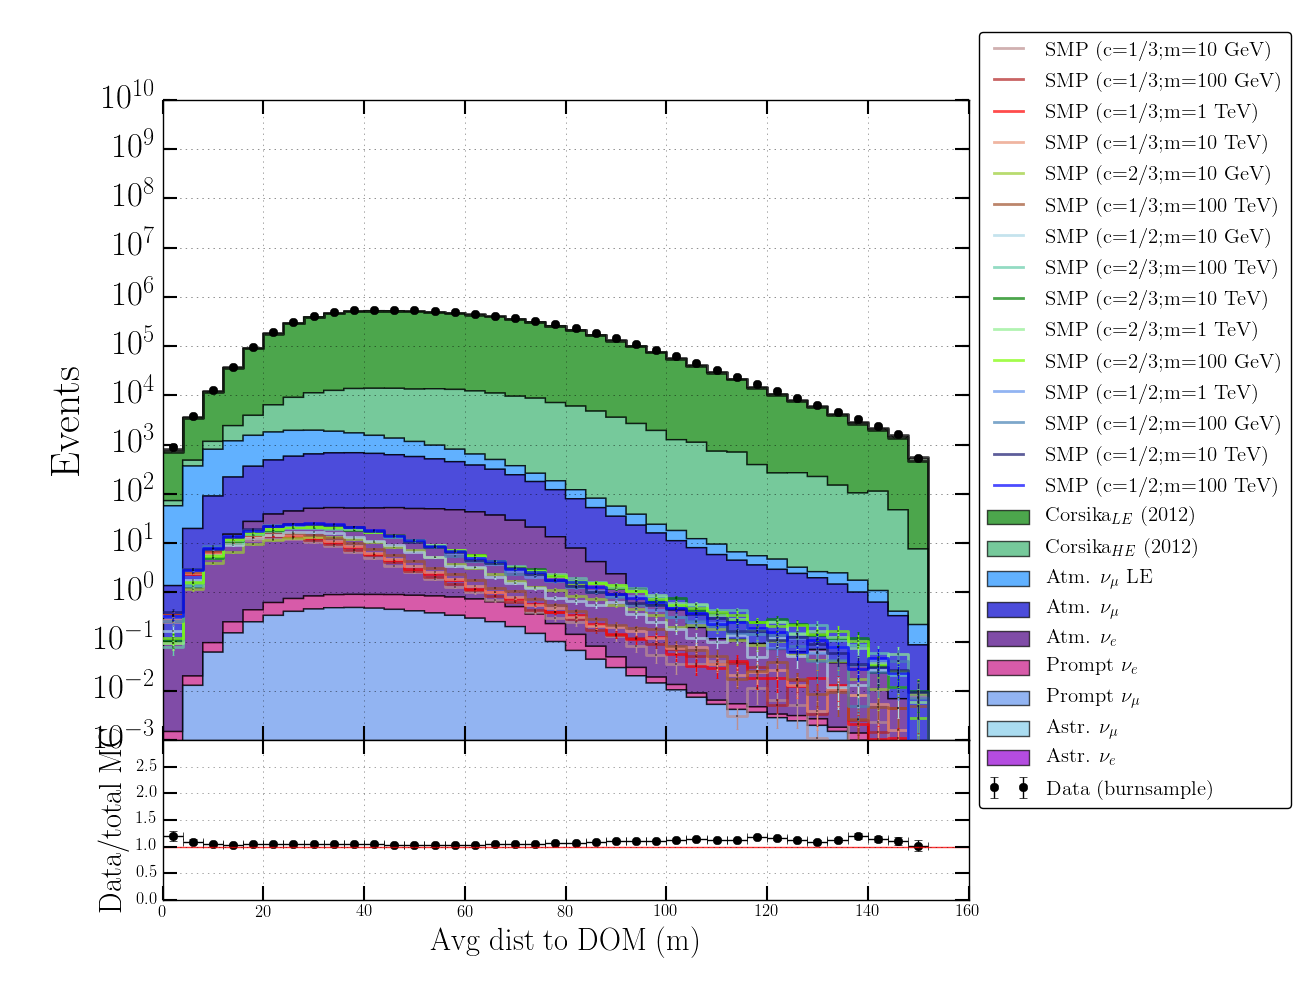
\includegraphics[width = 0.9\textwidth]{chapter8/img/1D_stack_avdistdom_150.png}
\caption{Distribution of the average distance of a hit DOM to the seed track. Signal events produce less light, making is less probable for DOMs far away from the track to record light pulses.}
\label{fig:commonvariablesavgdistdom150}
\end{figure}

\paragraph{EmptyHits}
Large values indicate that the track is sparse, with two or more clusters of hits that are far away from each other. Background events are not expected to produce long tracks with large parts of missing hits and therefore have much larger contribution at lower values. This is shown in Figure \ref{fig:commonvariablesemptyhits100}.

\begin{figure}
\centering
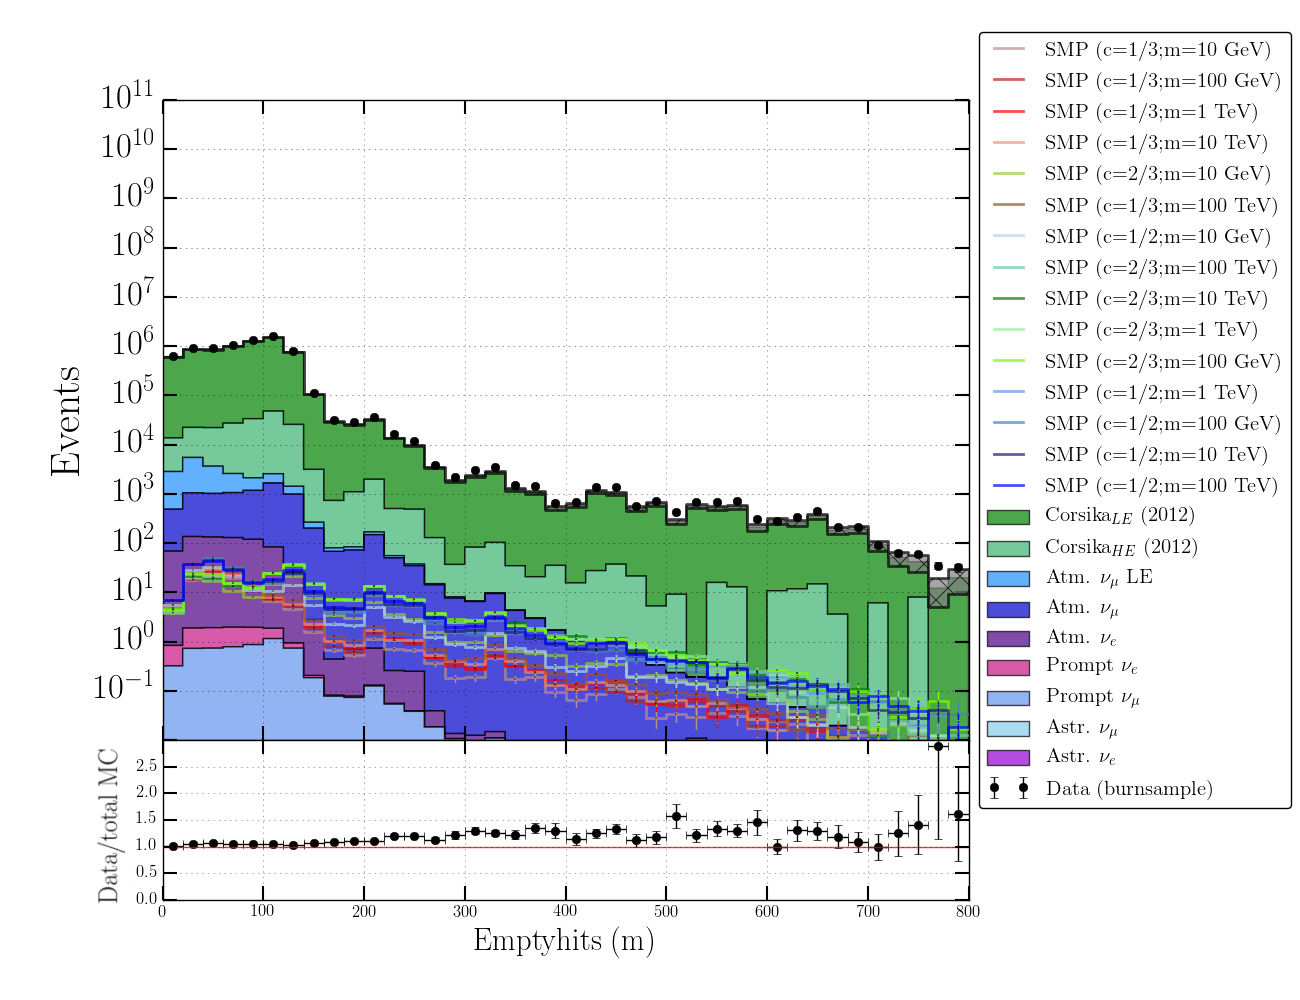
\includegraphics[width = 0.9\textwidth]{chapter8/img/1D_stack_emptyhits_100.png}
\caption{Distribution of the length of empty hits along a track. Dim signal events show longer tails in the distribution than the backgrounds.}
\label{fig:commonvariablesemptyhits100}
\end{figure}

\paragraph{COG Separation}
The distance between the COG of the first and last quartile of hits is expected to be large for throughgoing tracks. Therefore, signal events should have a larger contribution at higher values. Background events are not expected to have large COG separations. This is shown in Figures \ref{fig:commonvariablestracksep150} and \ref{fig:commonvariablestracksep50}.

\begin{figure}
\centering
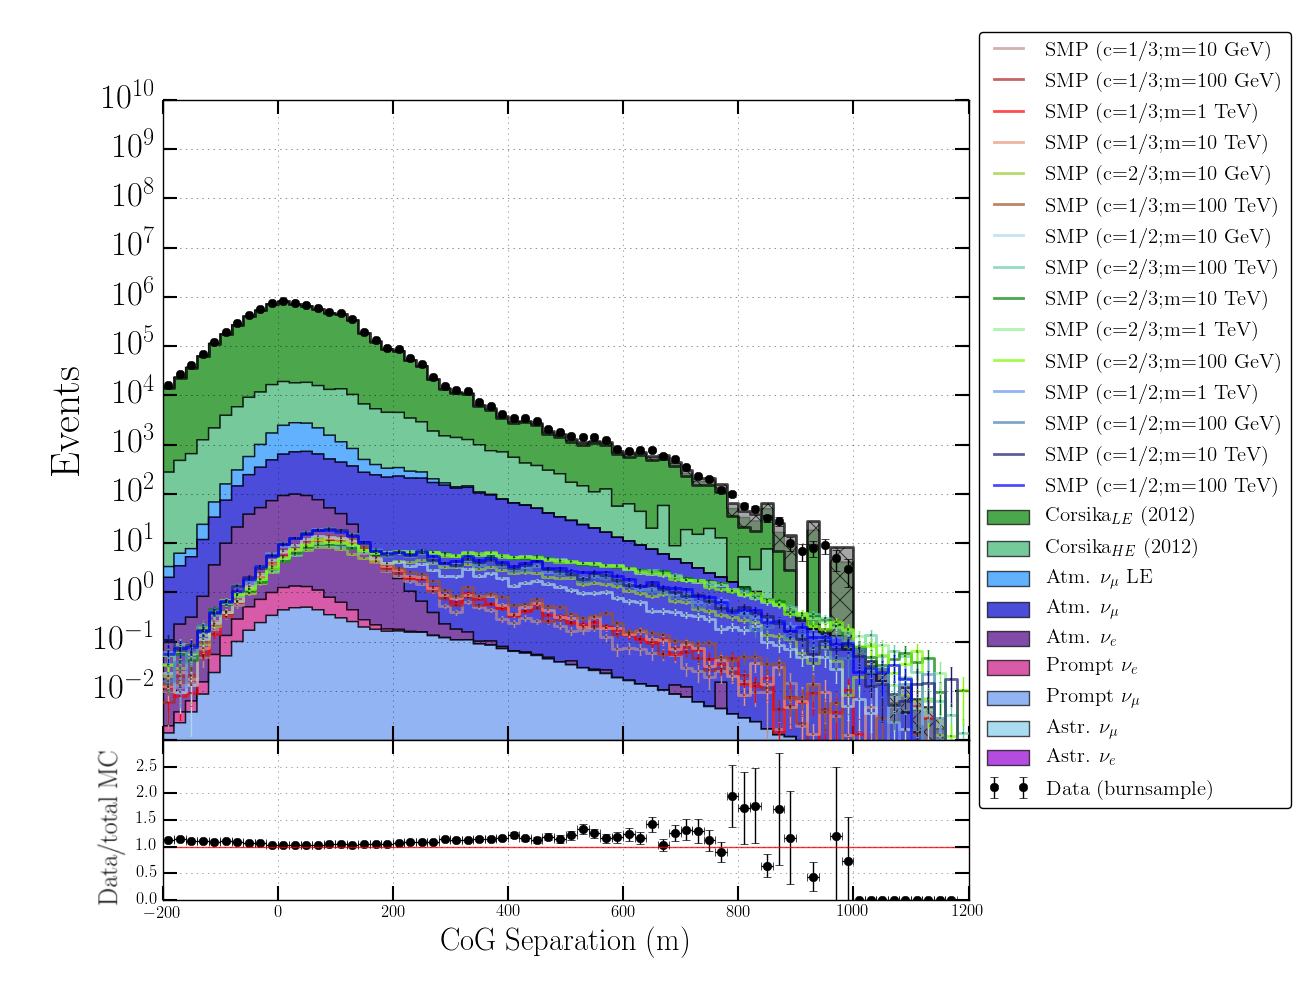
\includegraphics[width = 0.9\textwidth]{chapter8/img/1D_stack_trackseparation_150.png}
\caption{Distribution of the TrackSeparation, or COG separation, signal events show longer tails in the distribution compared to muons from air showers, as expected. A cylinder radius of 150 m was used.}
\label{fig:commonvariablestracksep150}
\end{figure}

\begin{figure}
\centering
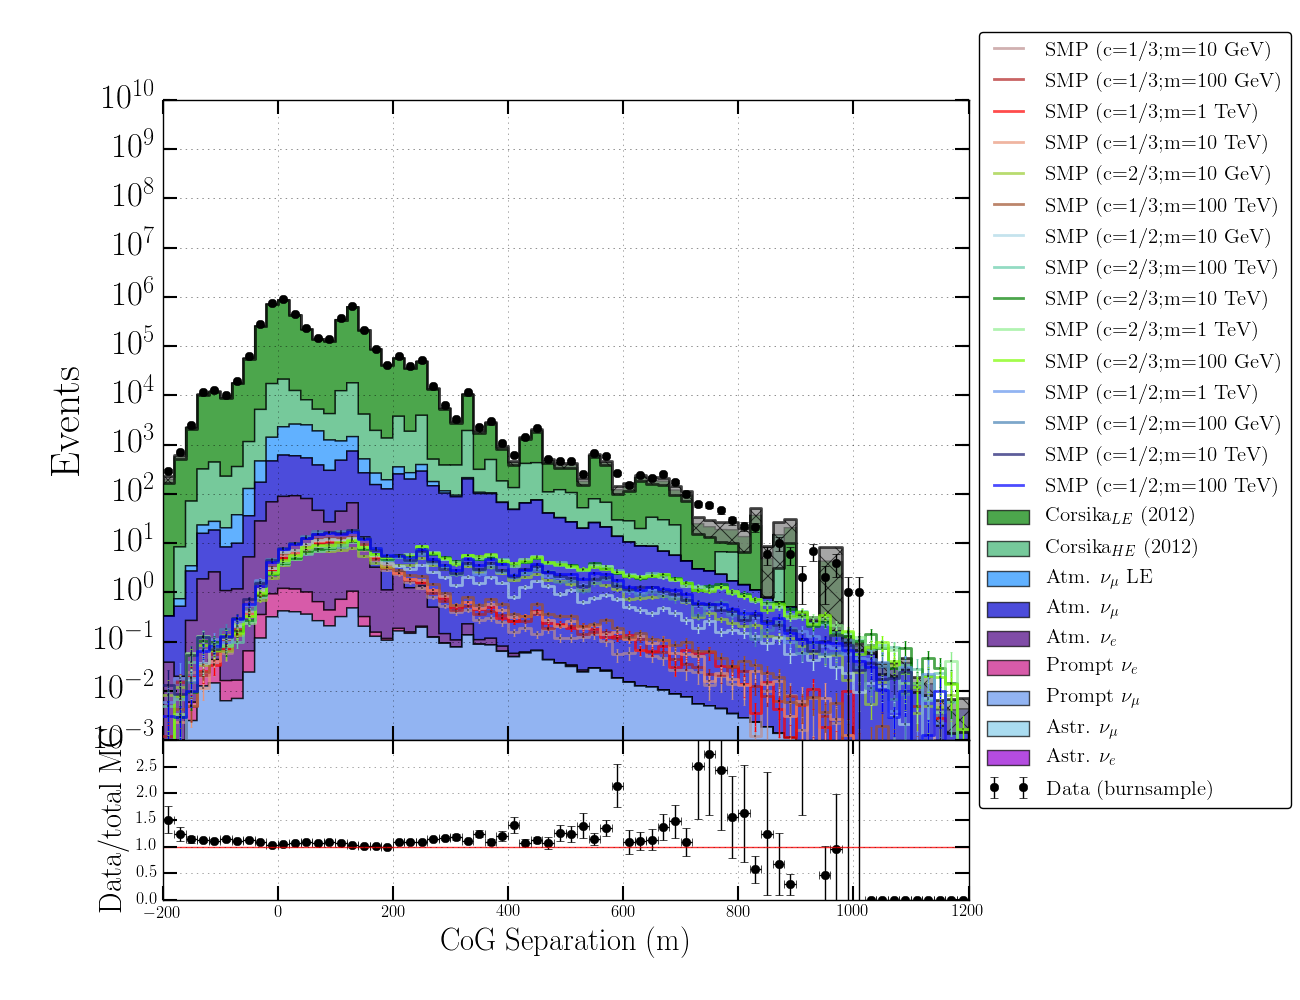
\includegraphics[width = 0.9\textwidth]{chapter8/img/1D_stack_trackseparation_50.png}
\caption{Distribution of the TrackSeparation, or COG separation, with a cylinder radius of 50 m.}
\label{fig:commonvariablestracksep50}
\end{figure}

\paragraph{TrackDistribution}
The smoothness of a track is rather difficult to be parameterized. The \textit{TrackDistribution} variable was developed and first used by P. Nie{\ss}en in his PhD thesis \cite{Niessen2001Search}. Signal events peak more at values close to zero. This is shown in Figure \ref{fig:commonvariablestrackdistr}.

\begin{figure}
\centering
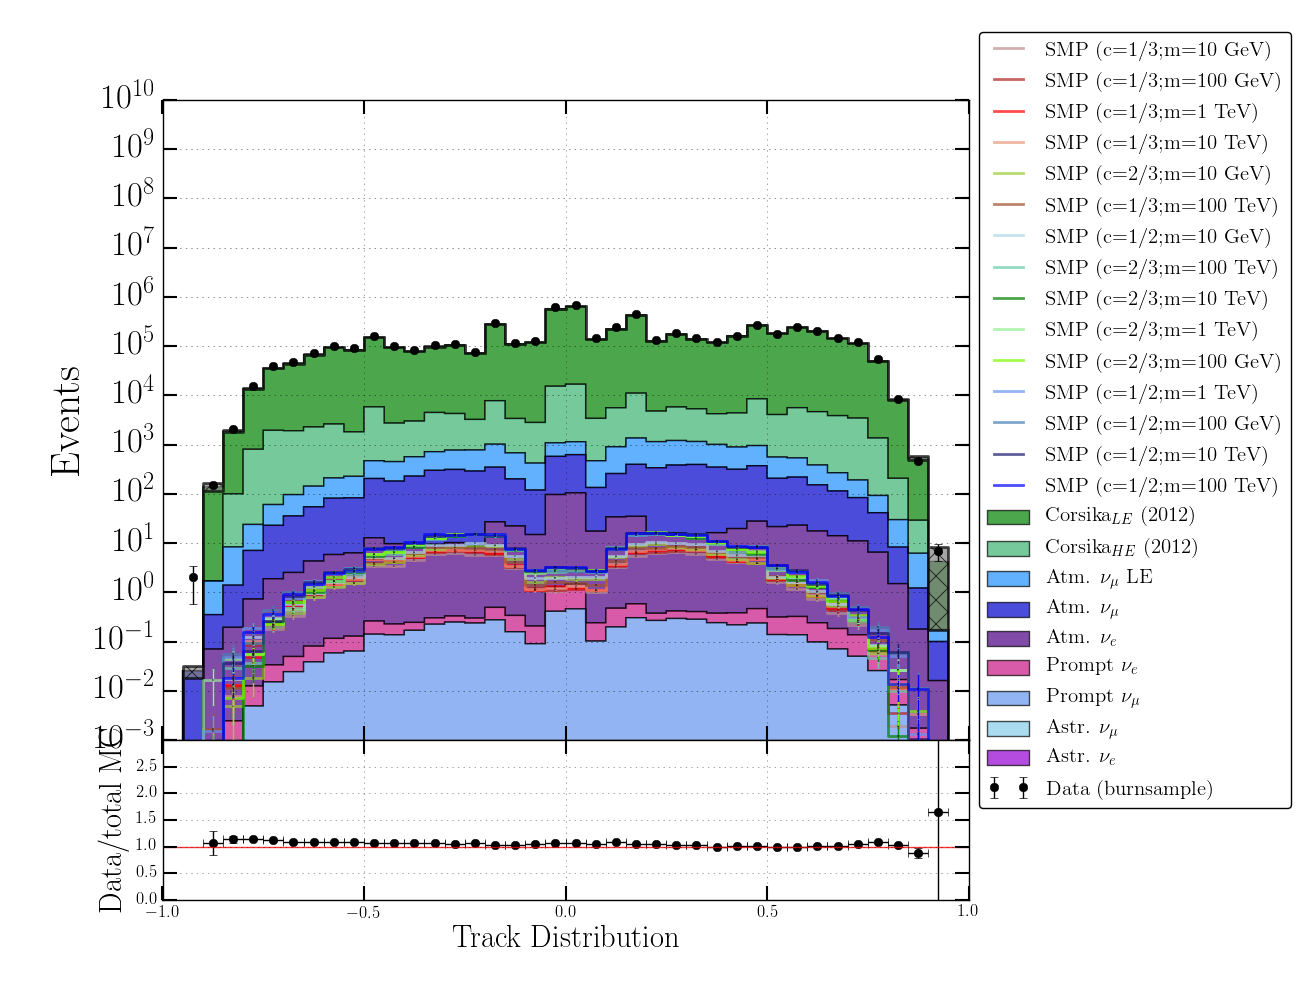
\includegraphics[width = 0.9\textwidth]{chapter8/img/1D_stack_trackdistribution_50.png}
\caption{Distribution of the smoothness of the track.}
\label{fig:commonvariablestrackdistr}
\end{figure}

\paragraph{ZTravel}
The average distance between the $z$-position of all DOMs and the $z$-position of the first quartile (in time) of all DOMs should be positive for upgoing tracks. Mis-reconstruction in air shower events therefore have a much larger contribution at lower values compared to signal events. This is shown in Figure \ref{fig:commonvariablesztravel}.

\begin{figure}
\centering
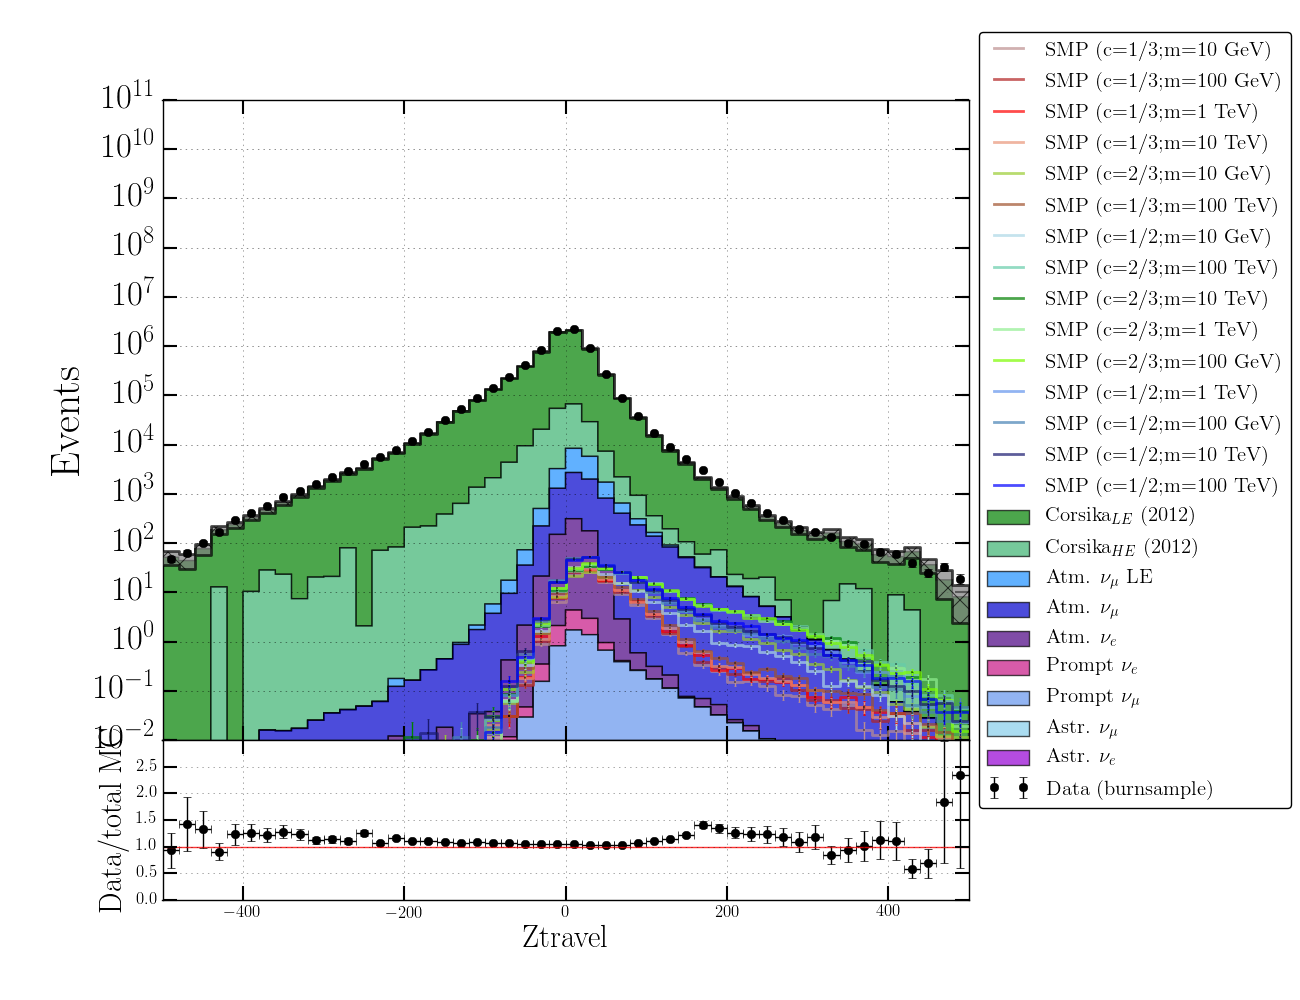
\includegraphics[width = 0.9\textwidth]{chapter8/img/1D_stack_ztravel.png}
\caption{Distribution of ZTravel. Negative values indicate downgoing tracks, explaining the differences in signal and muons from air showers.}
\label{fig:commonvariablesztravel}
\end{figure}

\paragraph{ZMax}
Upgoing tracks should have large \textit{ZMax} variables. Low values for signal events mostly consist of corner-clippers, corridor events, and events that did not trigger DOMs in the upper layer of the detector due to the low light yield. Muons from air shower events often stop in the top of the detector. This explains the large contribution at high values for air showers. The dip just below the origin is due to the dust layer (see Section \ref{sec:ice}). This is shown in Figure \ref{fig:commonvariableszmax}.

\begin{figure}
\centering
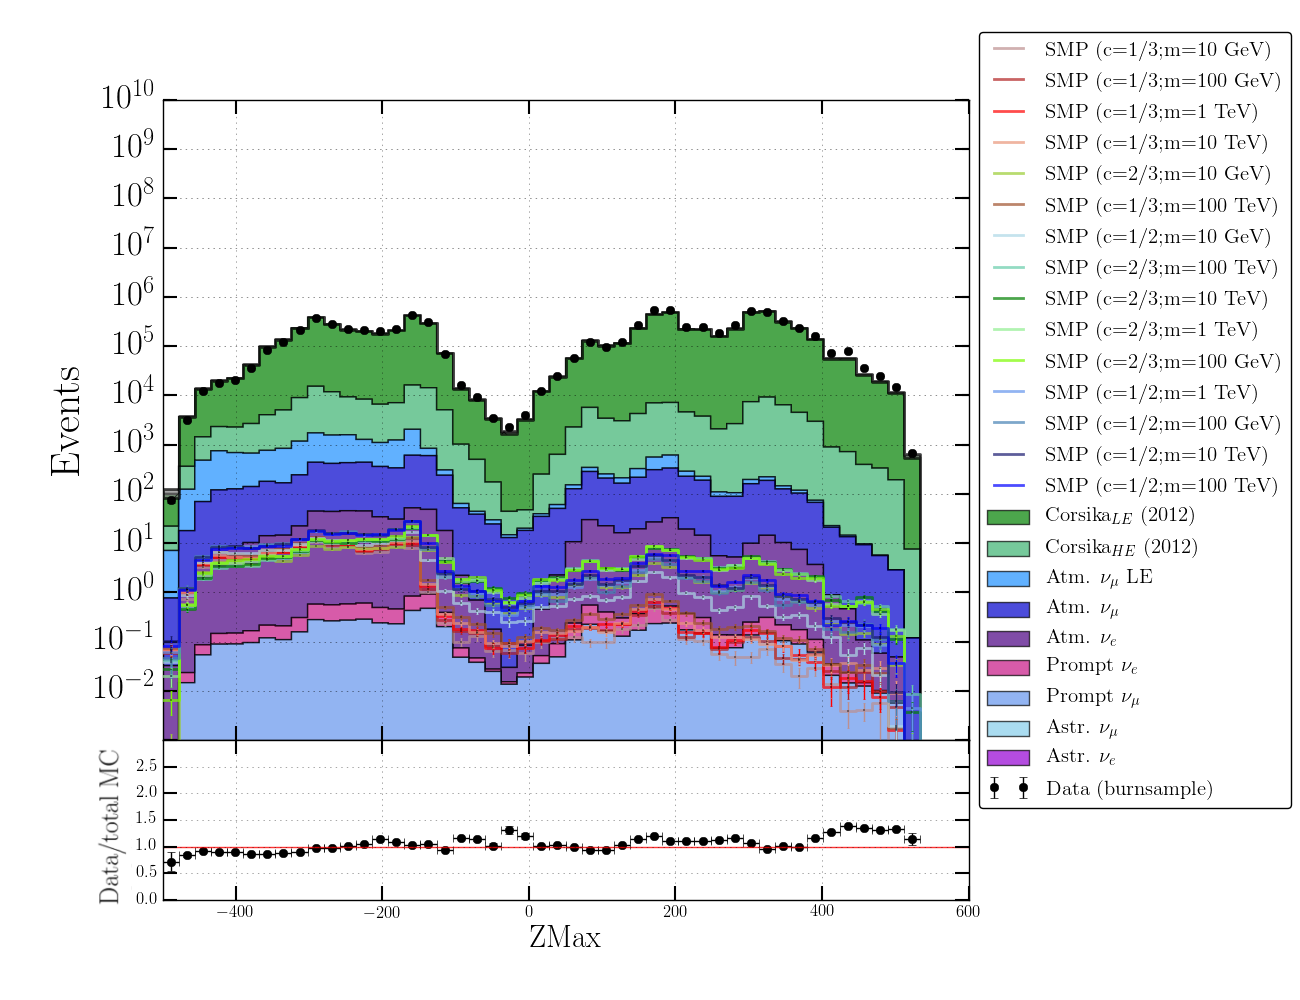
\includegraphics[width = 0.9\textwidth]{chapter8/img/1D_stack_zmax.png}
\caption{Distribution of ZMax. The dip slightly below the origin is due to the dust layer.}
\label{fig:commonvariableszmax}
\end{figure}

\paragraph{ZPattern}
This variable is described in more detail in Table \ref{tab:commonvariables}. Upgoing tracks result in positive values, making the variable a tool to discriminate from mis-reconstructed muons from air showers. This is shown in Figure \ref{fig:commonvariablesztravel}.

\begin{figure}
\centering
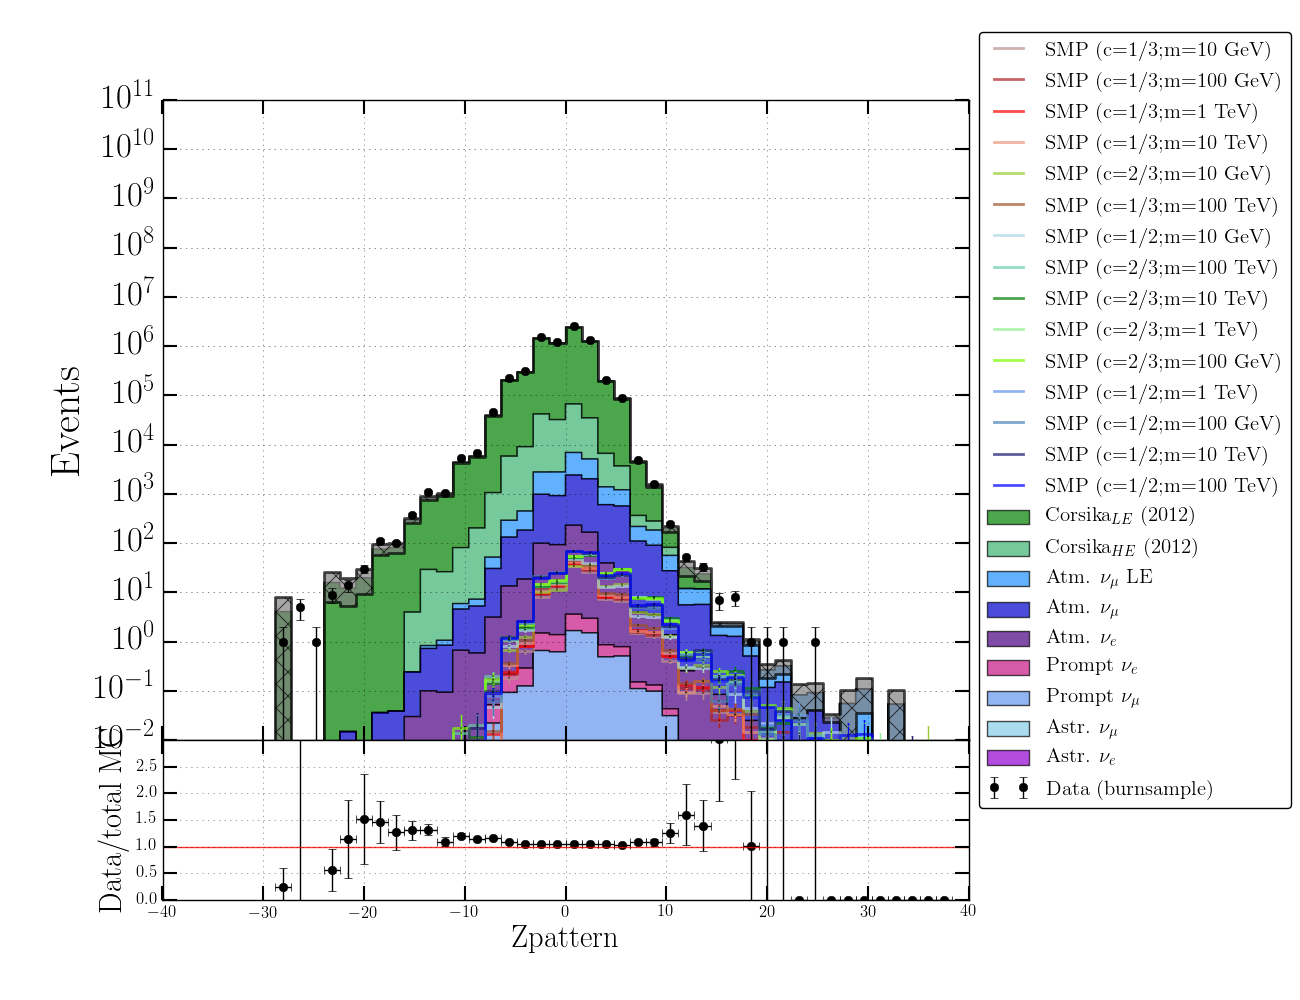
\includegraphics[width = 0.9\textwidth]{chapter8/img/1D_stack_zpattern.png}
\caption{Distribution of the ZPattern of a track. Negative values indicate downgoing tracks, explaining the different behavior in signal and background.}
\label{fig:commonvariableszpattern}
\end{figure}


\subsubsection{Millipede variables}
The \texttt{Millipede} toolkit was introduced in Section \ref{subsec:millipede}, where it was explained how energy depositions could be estimated from the light seen by the individual DOMs. Constructing multiple variables from this toolkit was the master thesis subject of Stef Verpoest. See Ref. \cite{steffthesis} for an elaborate explanation. The variables that were used in this analysis are explained below. Figure \ref{fig:millipedeoutput} shows how one fit was performed and can be helpful to explain the variables. The \texttt{Millipede} algorithm tries to estimate the energy that is deposited along a track from secondary interactions. The track is subdivided in segments of 15 m long. These deposits can be very small (most of the light originates from the primary particle at low energies), but still hold some information. In the example, we see that an SMP particle had several energy deposits along the track (green lines). The algorithm estimated that more energy deposits occurred close to the true deposits (that are known from the Monte Carlo samples). From this \texttt{Millipede} fit, several variables are constructed.

\begin{figure}
\centering
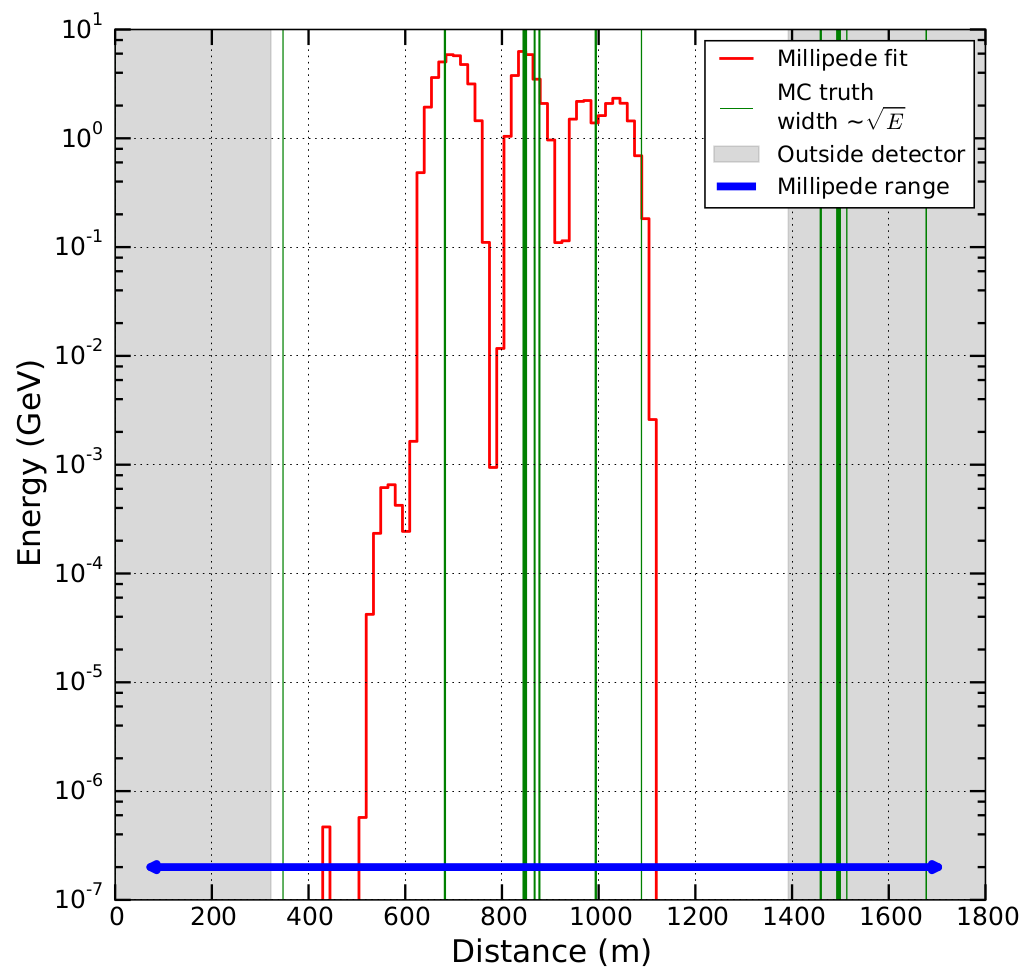
\includegraphics[width=0.6\textwidth]{chapter8/img/millipedeStef.png}
\caption{Output of a \texttt{Millipede} fit for a simulated SMP with charge $\frac{1}{3}$ and mass 10 GeV. The x-axis shows the distance the particle traveled and starts after the first energy loss event. The fit tries to estimate the energy deposited in 15 m track segments. As a comparison, the true positions of energy deposits from the MC simulation are shown in green. Locations outside the detector are shaded in grey.}
\label{fig:millipedeoutput}
\end{figure}

\paragraph{Mean loss}
The most straightforward use of the estimated energy loss rate is by taking the mean value and is referred to as \textit{Mean\_dEdX}. As can be seen from Figure \ref{fig:allmillipedevarmean}, the distribution of SMPs peaks at lower values than known backgrounds, as expected. Energy losses that are reconstructed to come from outside the detector are removed. 

Due to the squared charge dependencies, an SMP of charge 1/3 is expected to have a relative energy loss difference to muons with a factor of 9, which is the case when comparing to muons from neutrino interactions. We don't really see an exact factor of 9 difference as the algorithms still \textit{assumes} that a muon is passing through. Still, a significant shift is visible. Atmospheric muons in this level are almost entirely the result of mis-reconstructions, corner clippers, etc. making a comparison not valid.
%Je wijkt af van de dEdX die je verwacht omdat je al voorgaande cuts hebt die kijken naar low E muons... 

\begin{figure}
\centering
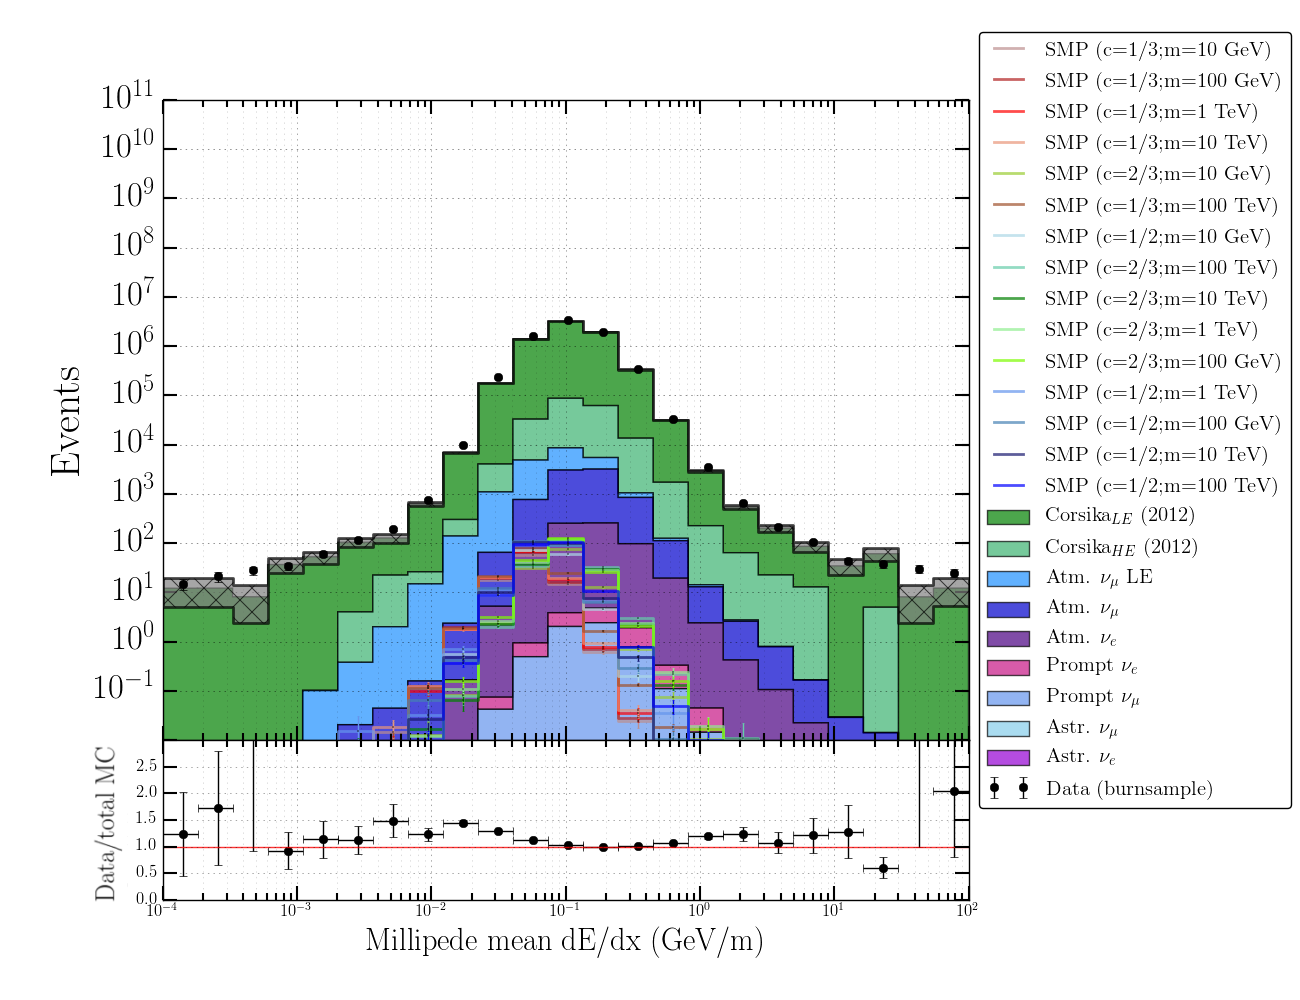
\includegraphics[width=0.9\textwidth]{chapter8/img/1D_stack_millipede_dedx_mean_nozeroes.png}
\caption{Distributions for the estimated mean energy loss from the \texttt{Millipede} toolkit.}
\label{fig:allmillipedevarmean}
\end{figure}

\paragraph{Uniformity}
Once the mean is computed, it is possible to count the number of times the energy distribution curve (red curve in Figure \ref{fig:millipedeoutput}) crosses the mean value. This variable therefore parameterizes the uniformity of the track. The reasoning behind discriminating signal events from background is that most SMPs will induce triggered hits that are distributed less uniformly due to the low amount of light that is produced. Particles therefore need to travel closer to a DOM to trigger a hit. In Figure \ref{fig:allmillipedevaruniformity}, we can see that the background distributions peak at lower values than the signal, which also has a slower dropoff. 

\begin{figure}
\centering
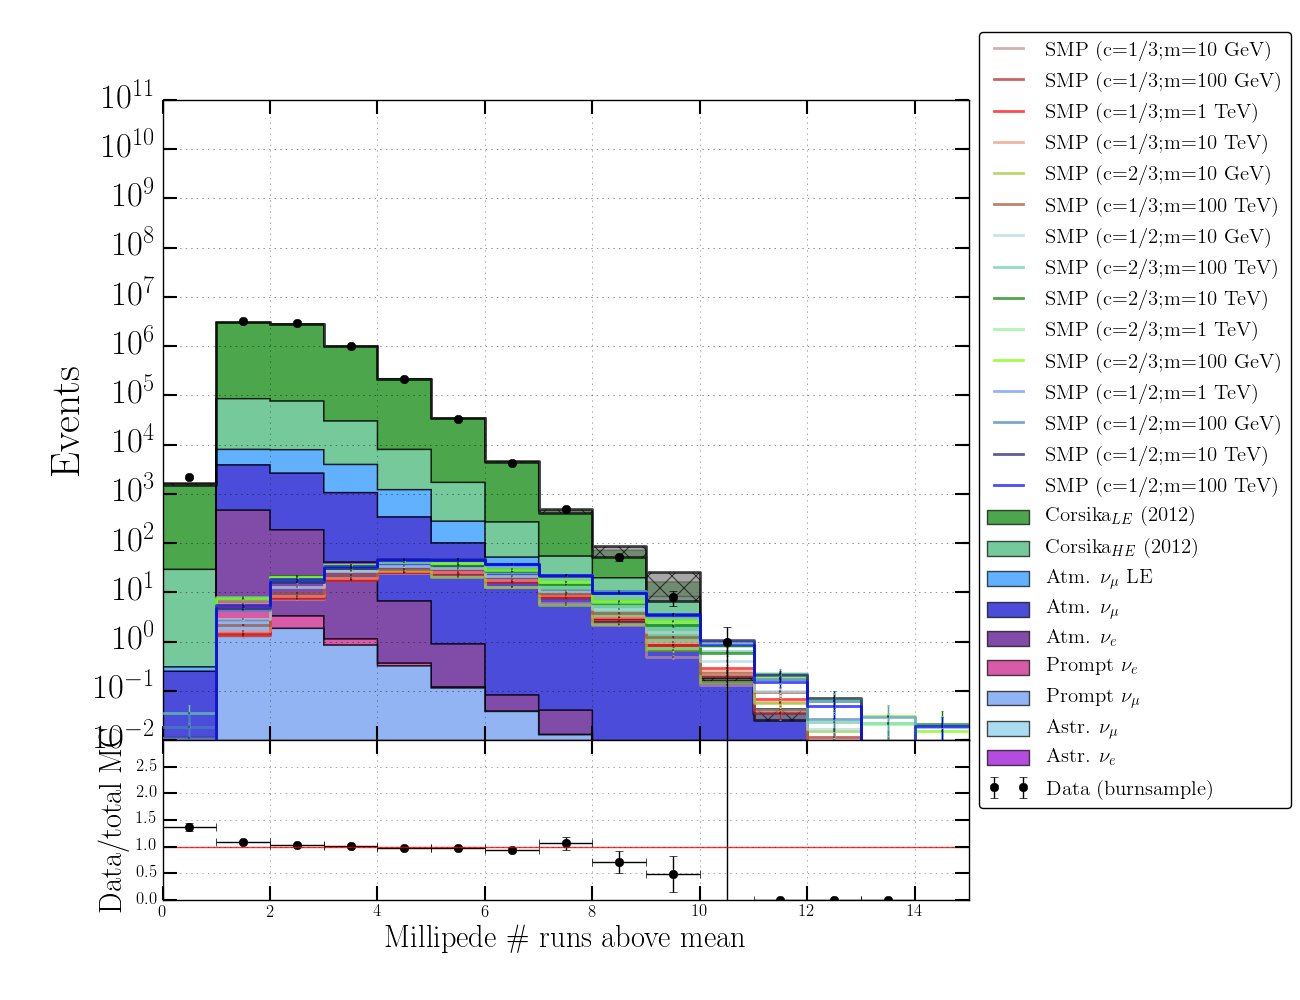
\includegraphics[width=0.9\textwidth]{chapter8/img/1D_stack_millipede_dedx_runsabovemean.png}
\caption{Distributions for the uniformity of the contained track.}
\label{fig:allmillipedevaruniformity}
\end{figure}

\paragraph{Track length}
Because of the lower energy loss, the SMP particles are also expected to travel larger distances than muons, supporting the idea to construct a variable that is sensitive to the distance traveled in the detector: a track length.

Since the tracks at this level induce very dim events, many segments from the \texttt{Millipede} output are reconstructed with zero energy. Therefore, it was chosen to use a certain part of the segments. The variable used here, \textit{TrackLength\_60}, returns the length were 60\% of the energy was deposited. It is the distance between the track segments where 20\% and 80\% of the energy was deposited. We expected to see larger tails in the distribution of Figure \ref{fig:allmillipedevartracklength} in the signal compared to the background. However, sub-optimal reconstructions result in bad millipede fits, giving a low and almost constant energy loss along the track. Additionally, coincident events that are not well separated also contribute to these events in the tail. Nonetheless, most of the background events result into low values, still making it a useful discriminative tool. 

\begin{figure}
\centering
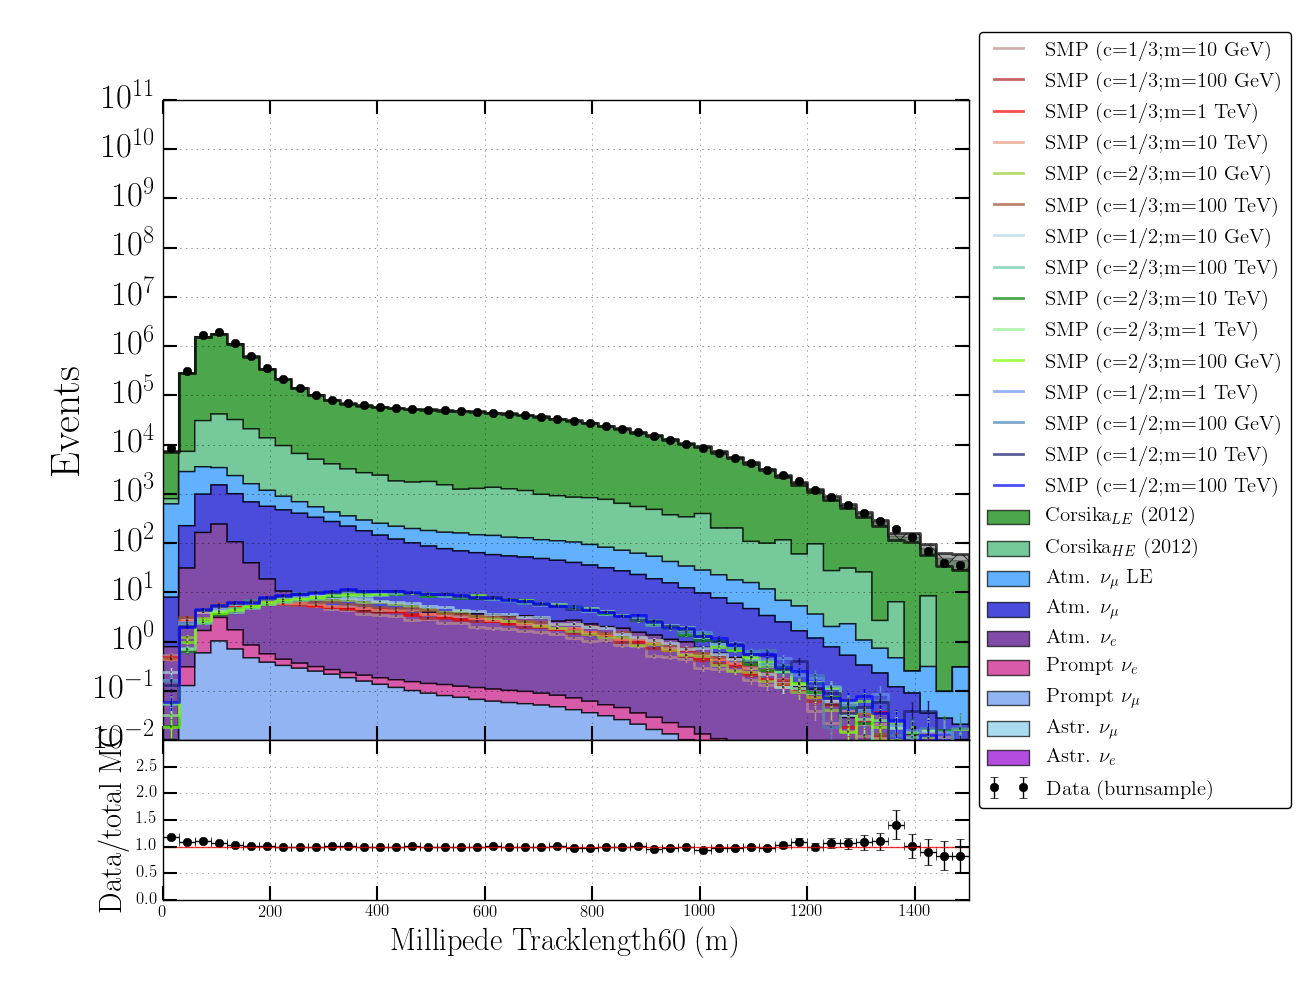
\includegraphics[width=0.9\textwidth]{chapter8/img/1D_stack_millipede_tracklength60.png}
\caption{Distributions for the track length of the particle where now the \texttt{Millipede} segments are used instead of the DOM pulses.}
\label{fig:allmillipedevartracklength}
\end{figure}


\subsubsection{New variables}

\paragraph{Speedratio}
In addition, new variables were constructed. One was adopted from Jan K\"unnen's Earth WIMP analysis \cite{kunnenthesis}. By looking at the ``speed ratio'' of the first to second and first to third HLC hits, it was possible to remove erroneous simulated detector noise, helping in data/MC agreement. In this analysis, it showed a modest addition to discriminating variables\footnote{In this analysis, data and MC seem to agree well, which is probably due to the newer and better simulations compared to a couple of years ago when the Earth WIMP analysis was done.} (as can be seen in Table \ref{tab:mrmrimportance}).  The \textit{Speedratio} is defined as

\begin{equation}
\frac{v_{12}}{v_{13}} = \frac{d\left( \textrm{HLC}_1,\textrm{HLC}_2 \right)/\Delta t\left(\textrm{HLC}_1, \textrm{HLC}_2\right)}{d\left(\textrm{HLC}_1, \textrm{HLC}_3 \right)/\Delta t\left(\textrm{HLC}_1,\textrm{HLC}_3 \right)},
\end{equation}
where $d\left( \textrm{HLC}_i,\textrm{HLC}_j \right)$ is the distance between the DOMs that recorded the $i$th and $j$th HLC hits. $\Delta t\left(\textrm{HLC}_1, \textrm{HLC}_2\right)$ is the difference in time of the $i$th and $j$th HLC hits. This distribution is expected to peak at a value of 1, which is the expected result if one assumes that the photons originate from a particle traversing in a straight line passing close to the DOMs. This is illustrated in Figure \ref{fig:newvariables1}.

\begin{figure}
\centering
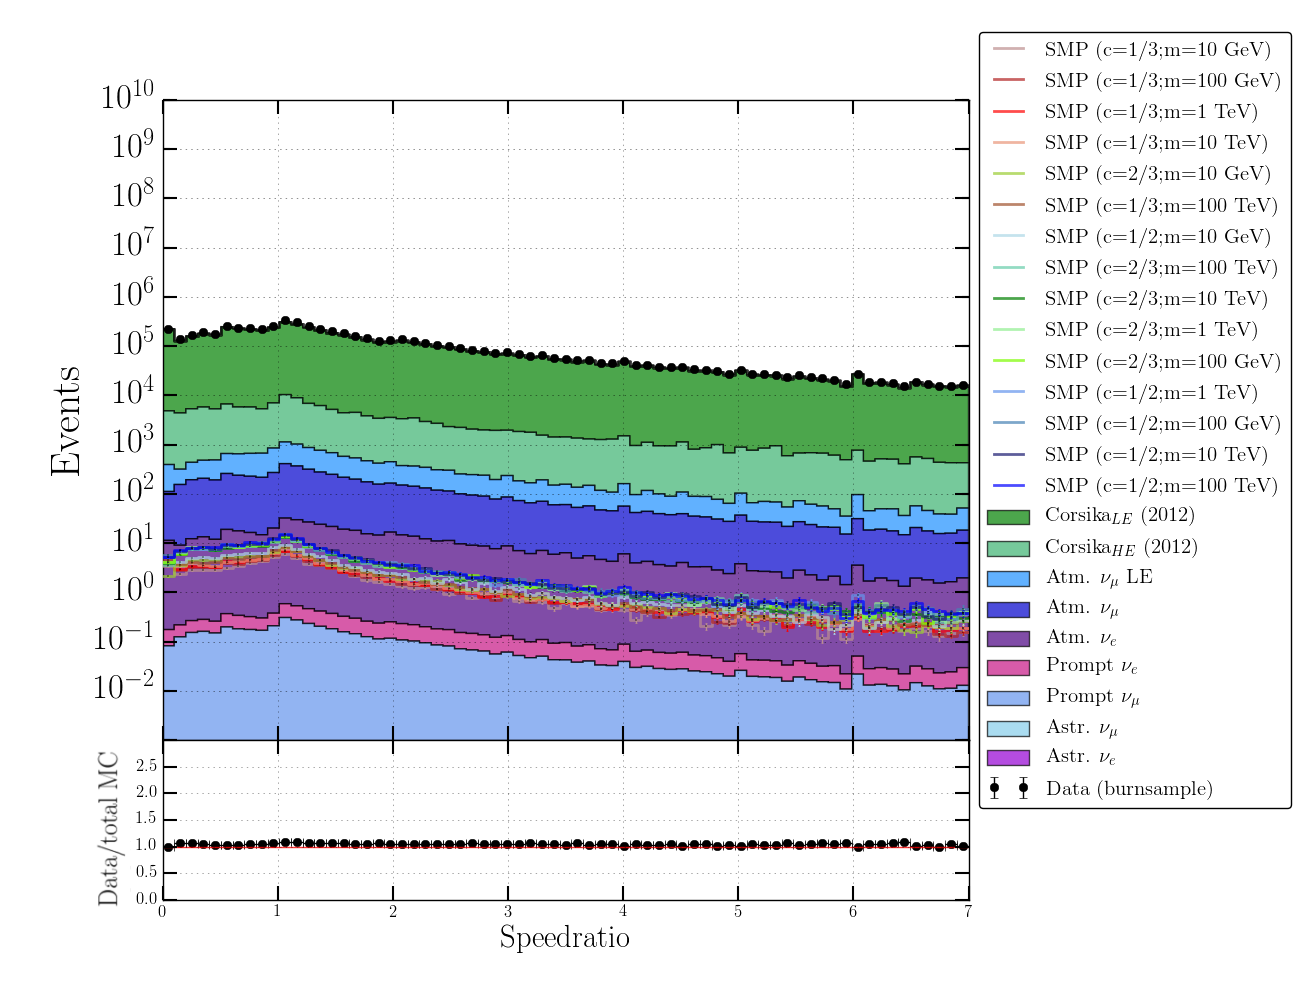
\includegraphics[width=0.9\textwidth]{chapter8/img/1D_stack_speedratio.png}
\caption{Distribution of the Speedratio variable.}
\label{fig:newvariables1}
\end{figure}


\paragraph{NewLength}
Because DC and IC pulses should not be mixed, essential information is lost regarding the length of a track. Many signal events are DC dominated (see Section \ref{subsub:commonvariables}), making those track length variables not optimal. This is especially the case for events that have both IC and DC hits and where clusters of hits are far away from each other (which is not expected from low-energetic muons). Low-energetic muons should, on average, not travel very far. High-energetic muons can have large tracks, but are almost completely removed with previous cuts that focus on dim tracks. In this analysis, new variables were constructed that use the MPE track reconstruction as a seed (\textit{seed track}). First, the event is required to have 

\vspace{2mm}
\begin{itemize}
\item \#DC pulses $\geq$ 4,
\item \#IC pulses $\geq$ 2,
\end{itemize}
\vspace{2mm}
since otherwise the hits would mainly consist of noise hits. Additionally,
pulses that lie within a cylinder (with the seed track as the center) are selected. The radius can be chosen, but is of the order of 50-150 meters. This radius is shown with a suffix after the variable (e.g. ``\_100''), if the radius is infinite (all pulses are used), the suffix is ``\_all''. 

Then the first/last quartile in DC hits and the first/last half of the IC hits are determined. For each quartile/half, one can easily calculate a COG. To determine the length of a track between four COGs, two have to be selected. The selection is based on the timing information on these COGs and given in the Table \ref{table:newlength}. An illustration how the NewLength variable is constructed is shown in Figure \ref{fig:newlength}\\

\begin{table}[]
\caption{Selection procedure which COGs should be used to compute a track length. $f, l, h \textrm{ and } q$ stand for first, last, half and quarter respectively. The left column shows possible timing conditions between IC and DC COGs. The right column indicates which COG is chosen as the first and which one as the last in the four different timing scenarios.}
\label{table:newlength}
\centering
\begin{tabular}{|l |c|}
\hline
\cellcolor[HTML]{F1A91E}Timing & \cellcolor[HTML]{F1A91E}COG$_1$ \\ \hline
$\textrm{DC}_{f,q} < \textrm{IC}_{f,h}$ & DC$_{f,q}$ \\ \hline
$\textrm{DC}_{f,q} \geq \textrm{IC}_{f,h}$ & IC$_{f,h}$ \\ \hline
\cellcolor[HTML]{F1A91E} & \cellcolor[HTML]{F1A91E}COG$_2$ \\ \hline
$\textrm{DC}_{l,q} > \textrm{IC}_{l,h}$ & DC$_{l,q}$ \\ \hline
$\textrm{DC}_{l,q} \leq \textrm{IC}_{l,h}$ & IC$_{l,h}$ \\ \hline
\end{tabular}
\end{table} 
 
\noindent Summarizing, the NewLength variable is another attempt in defining the length of the track in the detector. The suffix ``\_z'' is used for the variable that only uses the $z$-coordinate. Negative values occur when the timing of the two selected COGs is inverted when compared to the seed track (e.g. if the seed track is downgoing but the first COG in time is located below the second) and are present when the reconstruction was not optimal.\\

\noindent The distributions of this variable are shown in Figures \ref{fig:newvariablesnewlength} and \ref{fig:newvariablesnewlengthallz}. Signal samples show larger contributions at higher values, showing that the variable is capable of extracting information about the length of a track for dim events. Muons from air shower events show many more low and negative values, as expected. Upgoing signal tracks can clearly be more easily distinguished from mis-reconstructed downgoing muons when only the $z$-coordinate is used.

\begin{figure}
\centering
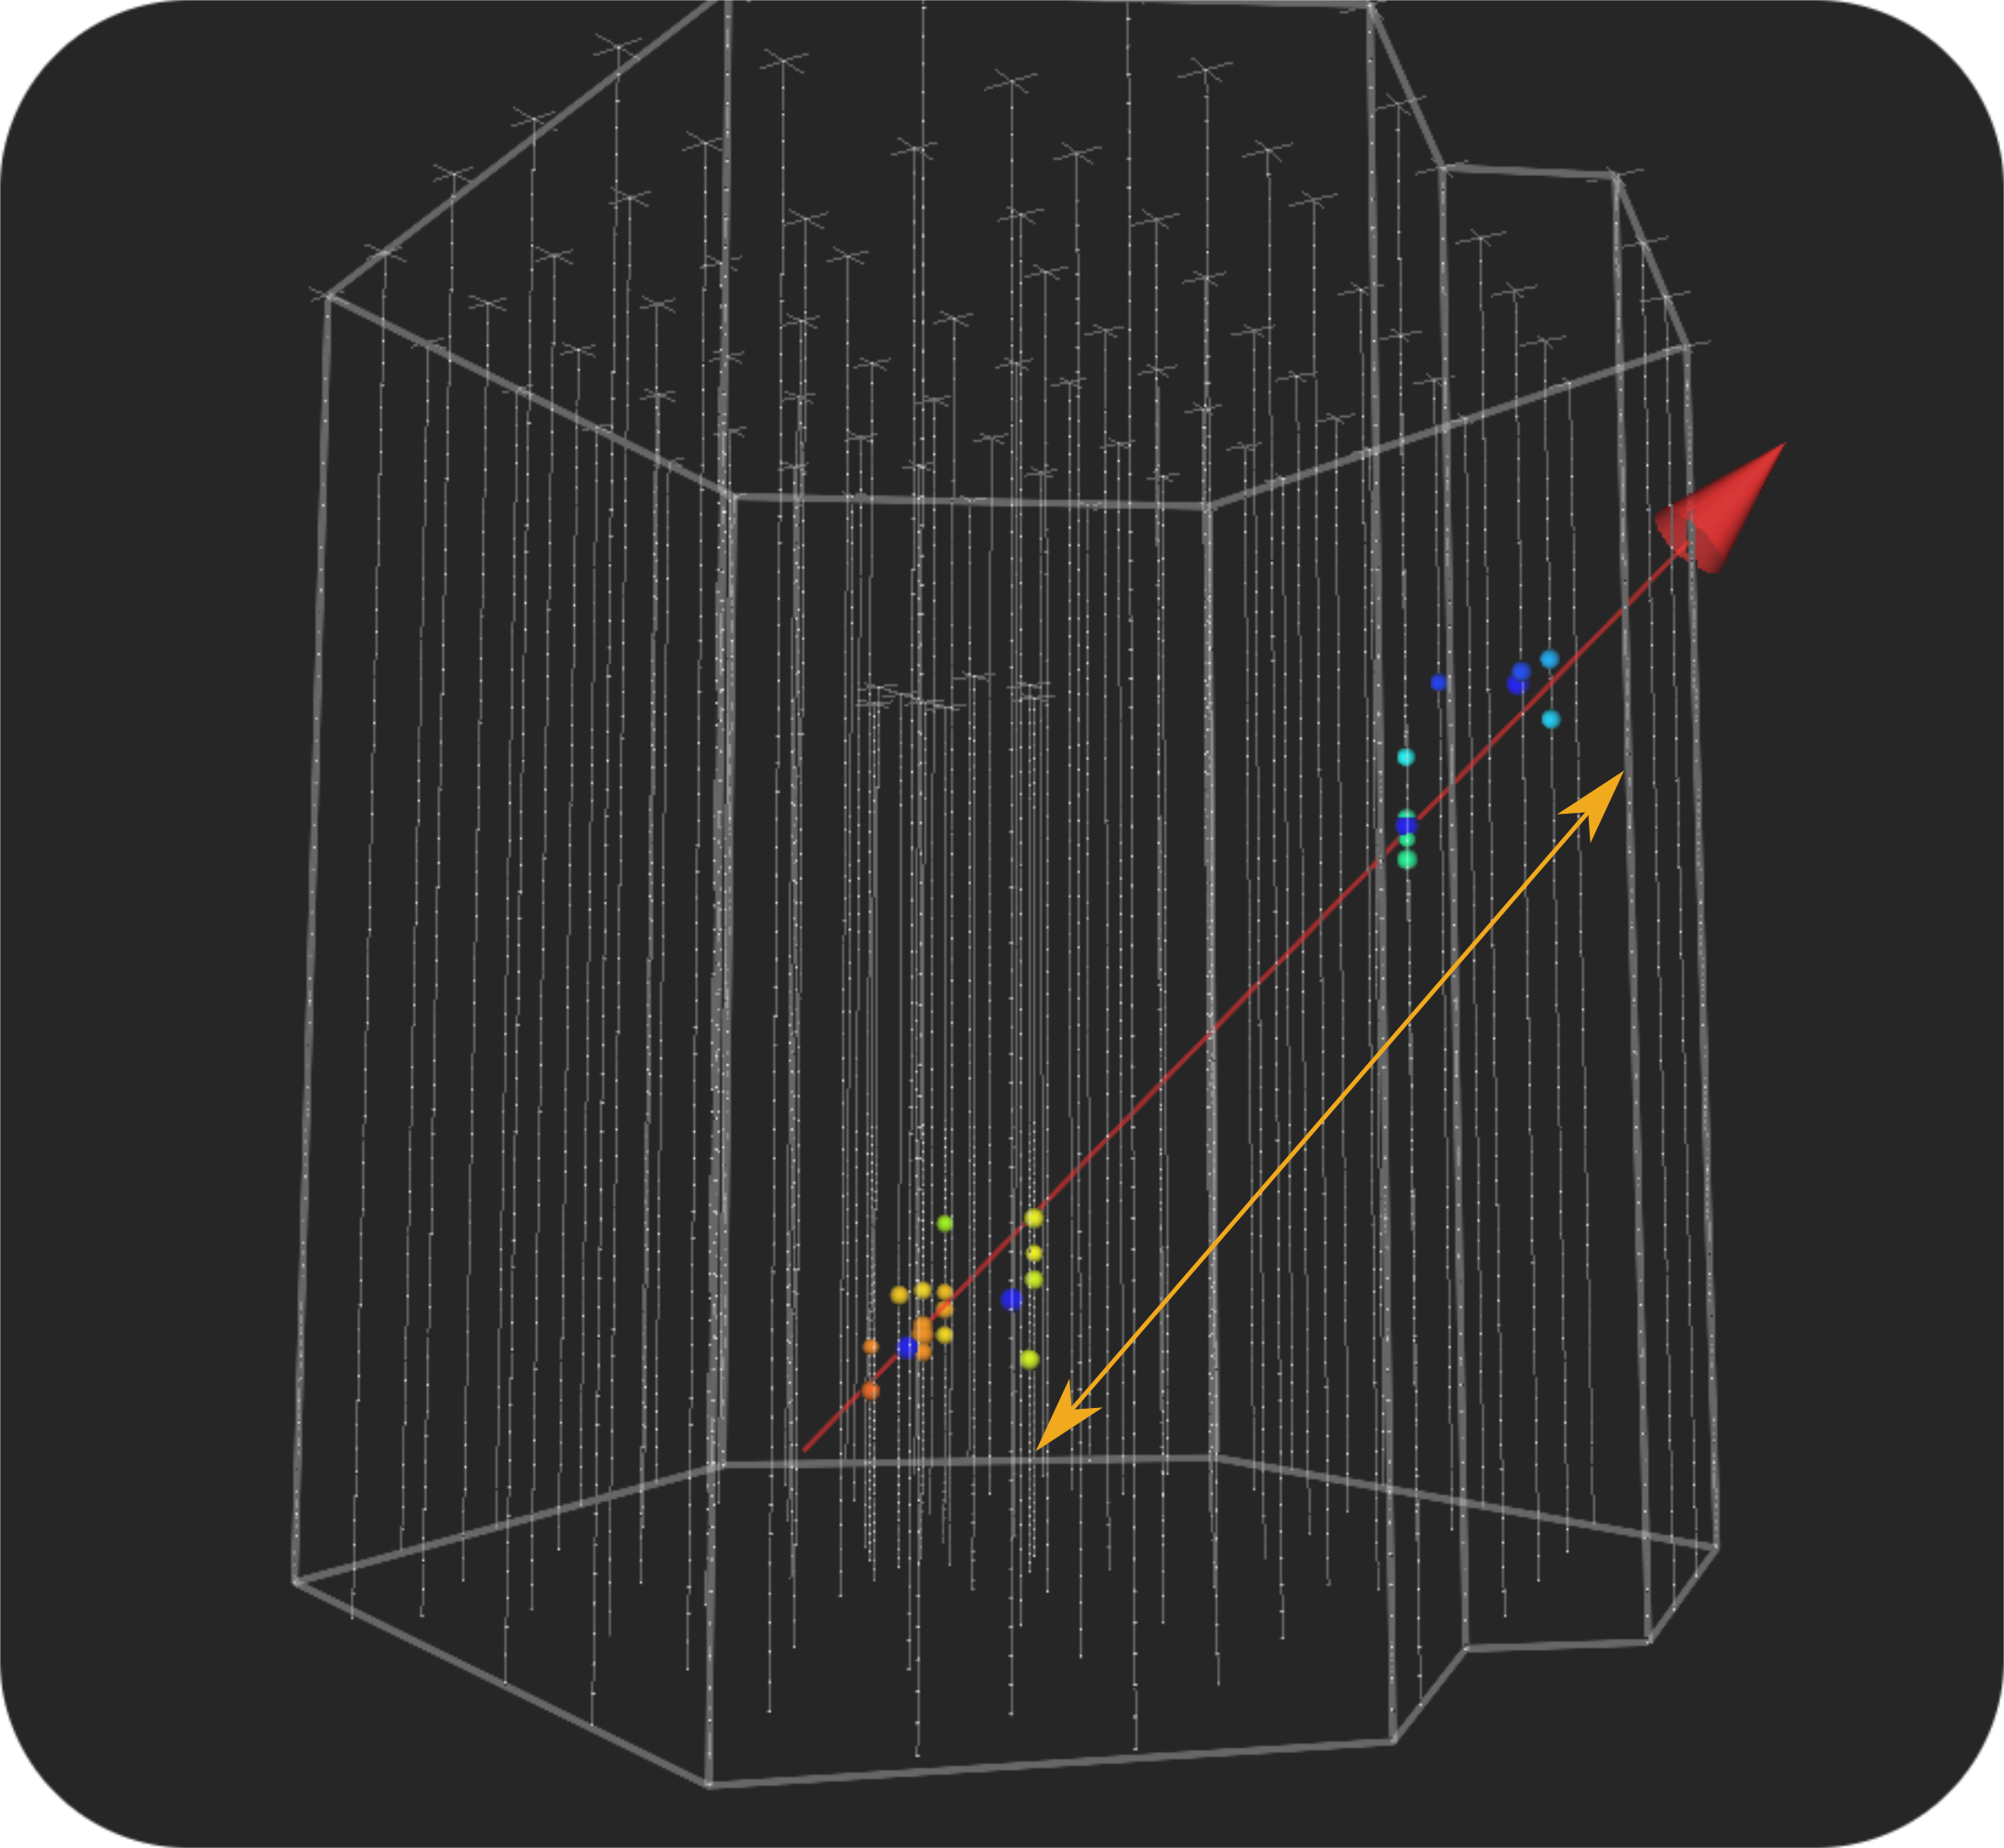
\includegraphics[width=0.6\textwidth]{chapter8/img/newlengthillustration_extra.png}
\caption{The NewLength variable is constructed by selecting the first quartile/half of the COGs of DC/IC and computing the distance from the last quartile/half of the COGs of DC/IC. Out of the four, the first and last in pulse time are chosen to compute the distance.}
\label{fig:newlength}
\end{figure}
 

\begin{figure}
\centering
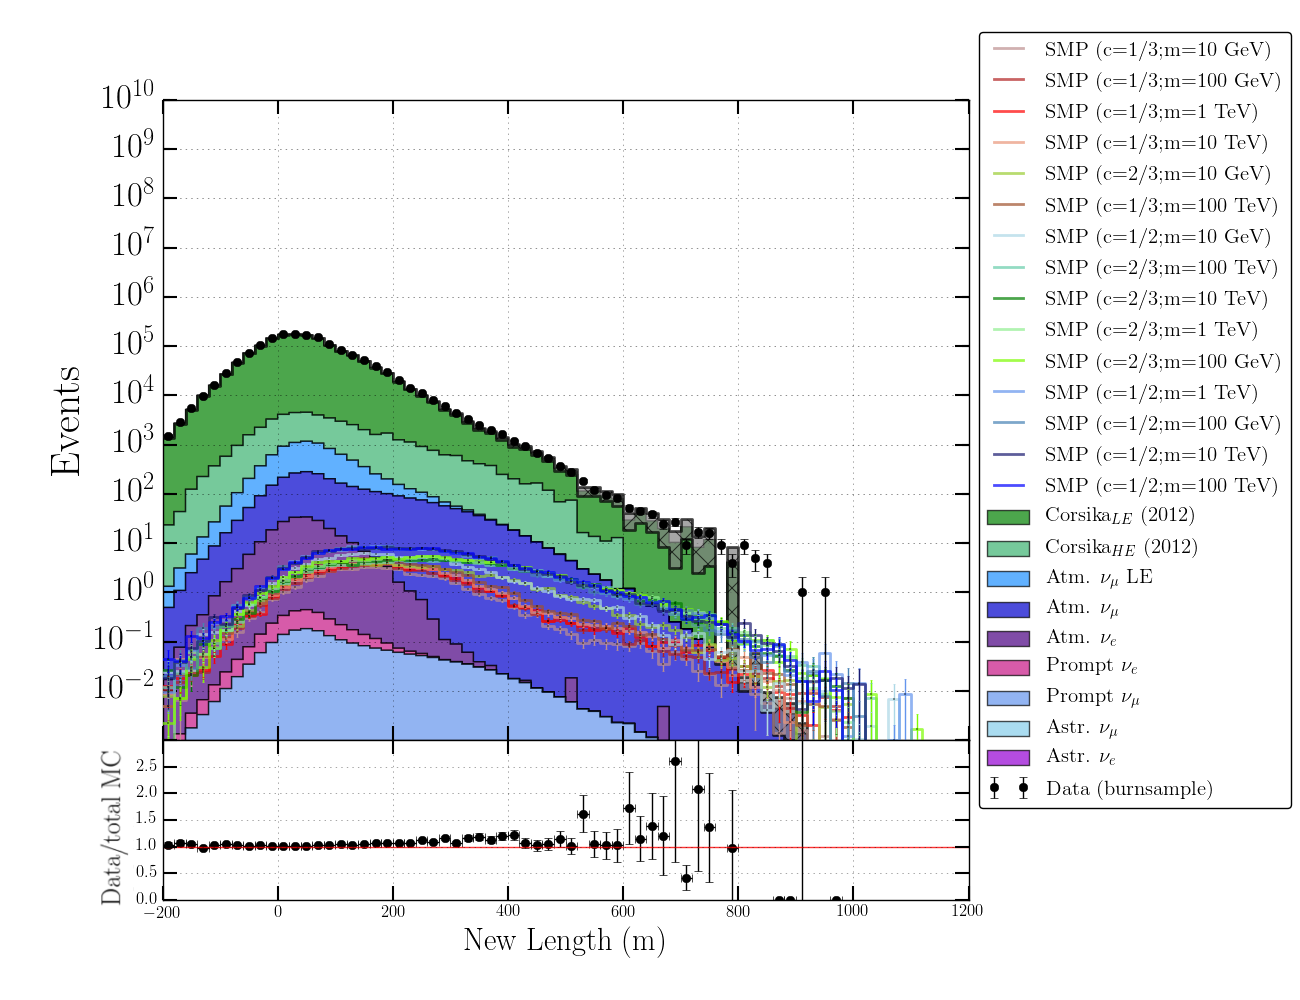
\includegraphics[width=0.9\textwidth]{chapter8/img/1D_stack_newlength_150.png}
\caption{Distribution of the New Length\_150 variable.}
\label{fig:newvariablesnewlength}
\end{figure}


\begin{figure}
\centering
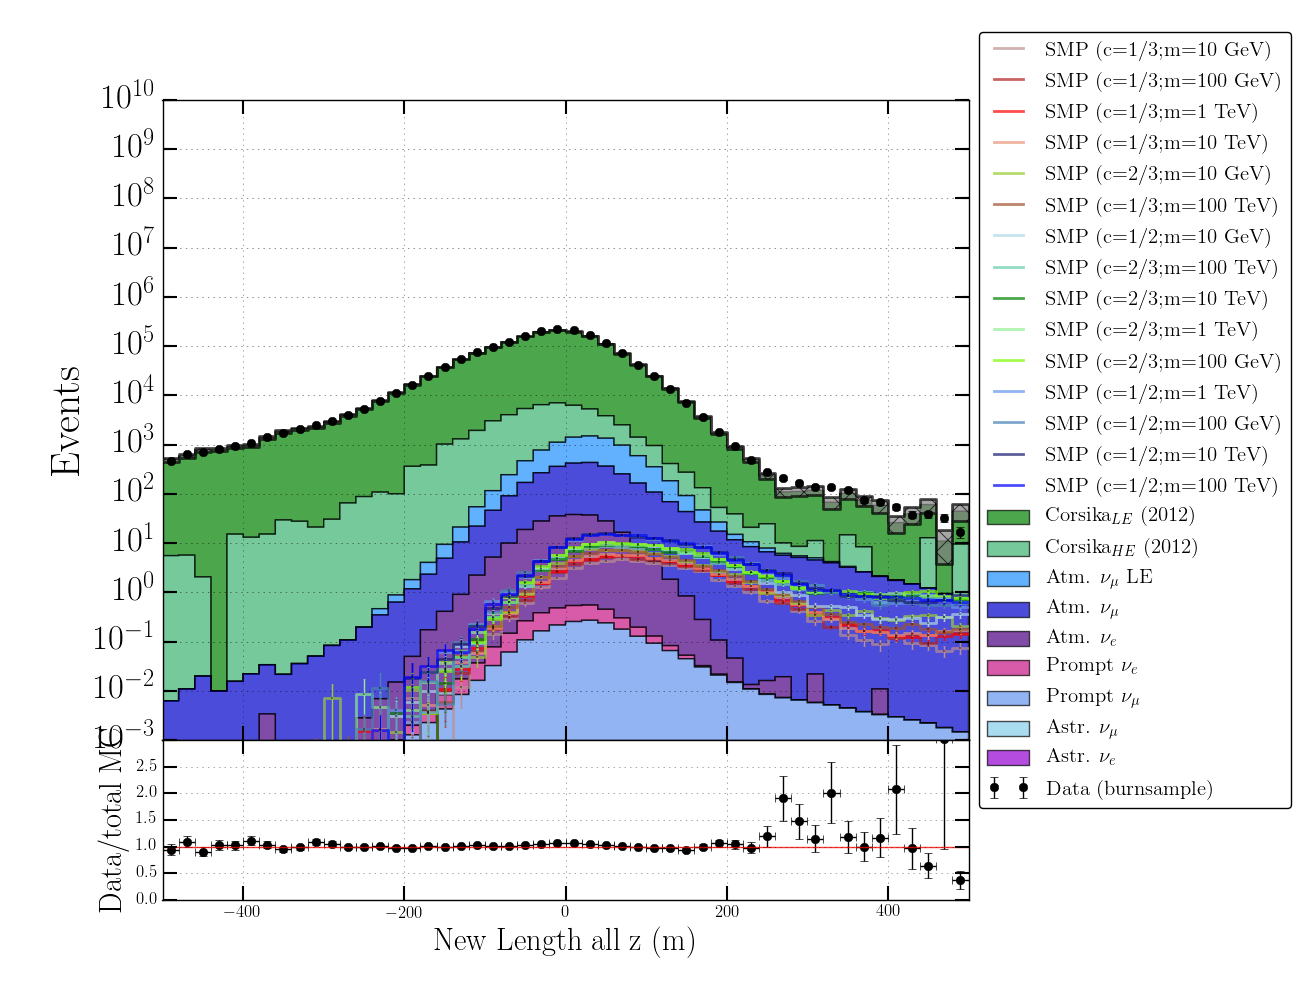
\includegraphics[width=0.9\textwidth]{chapter8/img/1D_stack_newlength_all_z.png}
\caption{Distribution of the New Length where we only focus on the $z$-coordinate.}
\label{fig:newvariablesnewlengthallz}
\end{figure}


\subsubsection{Other variables}
\label{subsub:other}
Additional to the 14 variables that were discussed in the previous sections, three extra variables were used in Level 5. These variables are constructed from the reconstruction techniques as discussed in Chapter \ref{ch:reconstruction}. They are briefly discussed below.

\paragraph{LineFit velocity}
The \texttt{LineFit} algorithm was explained in Section \ref{subsec:lf}. There, we discussed how the velocity of a particle that produces a track in the detector can be estimated. The velocity for a relativistic particle is equal to $\approx$0.3 m/ns. However, because of the simplistic assumptions in the module, we expect the distribution to peak at the velocity of light in vacuum, but have a broad distribution. This can be seen in Figure \ref{fig:remainingvariableslf}. Muons from muon-neutrinos and signal events indeed peak at the velocity of light in vacuum, as expected.

\paragraph{Paraboloid sigma}
The \texttt{Paraboloid} module was explained in Section \ref{subsec:paraboloid}. The \textit{Paraboloid $\sigma$} has low values for tracks that have a small uncertainty on the reconstructed direction. Longer tracks from SMPs should have lower uncertainties than the short tracks that are mostly expected from backgrounds. This can be seen in Figure \ref{fig:remainingvariablespara}.

\paragraph{SPE zenith}
After cleaning with the \texttt{IceHive} module, the SPE and MPE reconstructions were re-applied. Negative values of $\cos\left(\theta\right)$ indicate upgoing tracks. There is only a small fraction of SMP tracks that are reconstructed as downgoing after cleaning with the \texttt{IceHive} module, whereas a much larger fraction of the air shower background is now (correctly) reconstructed as downgoing. This can be seen in Figure \ref{fig:remainingvariableszenith}.

\begin{figure}
\centering
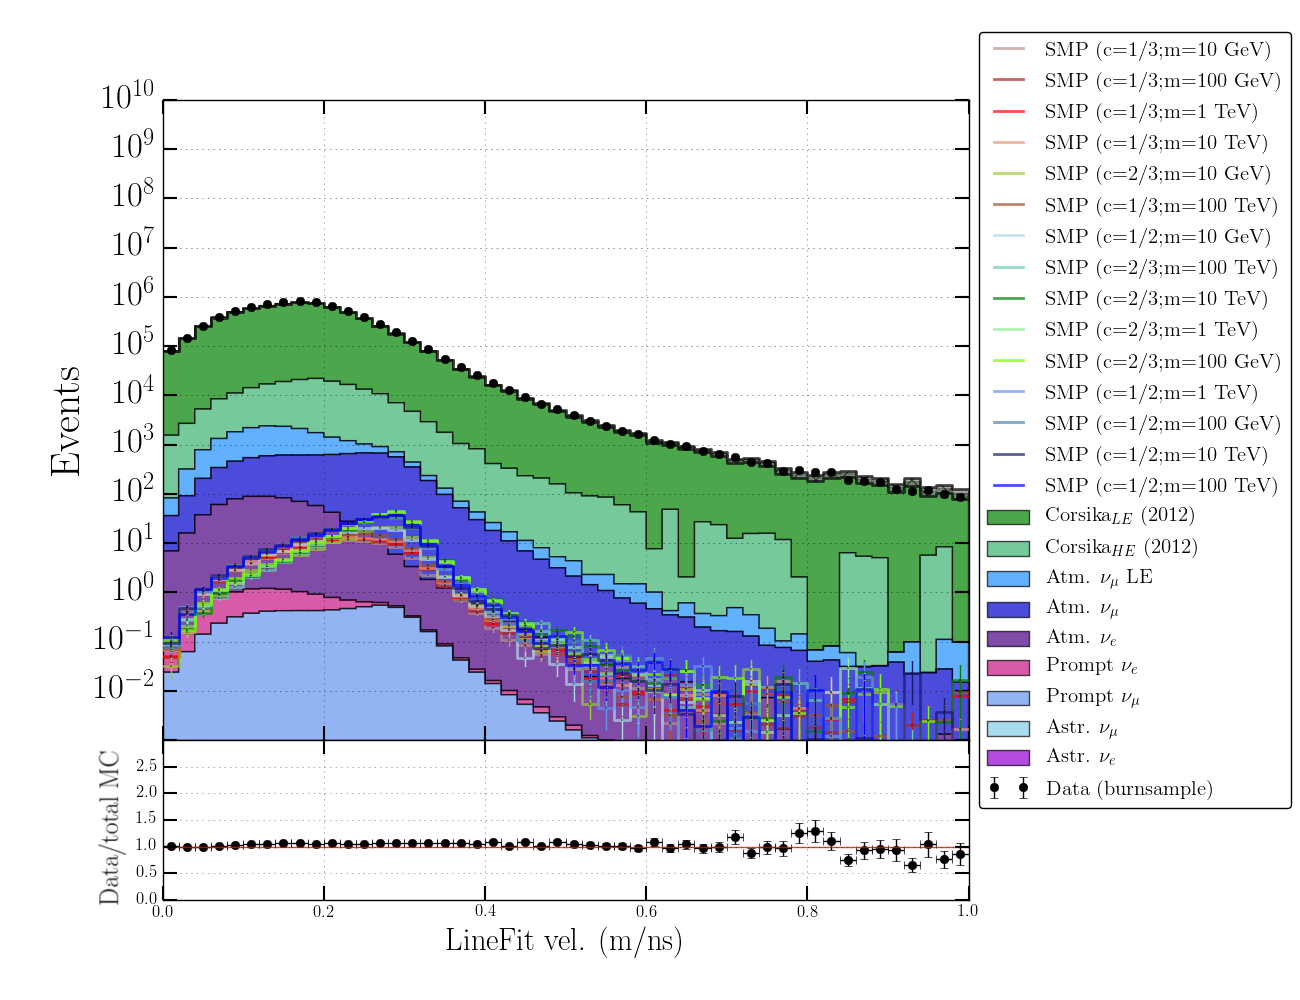
\includegraphics[width=0.9\textwidth]{chapter8/img/1D_stack_linefitvelocity}
\caption{Velocity distribution of the \texttt{LineFit}.}
\label{fig:remainingvariableslf}
\end{figure}


\begin{figure}
\centering
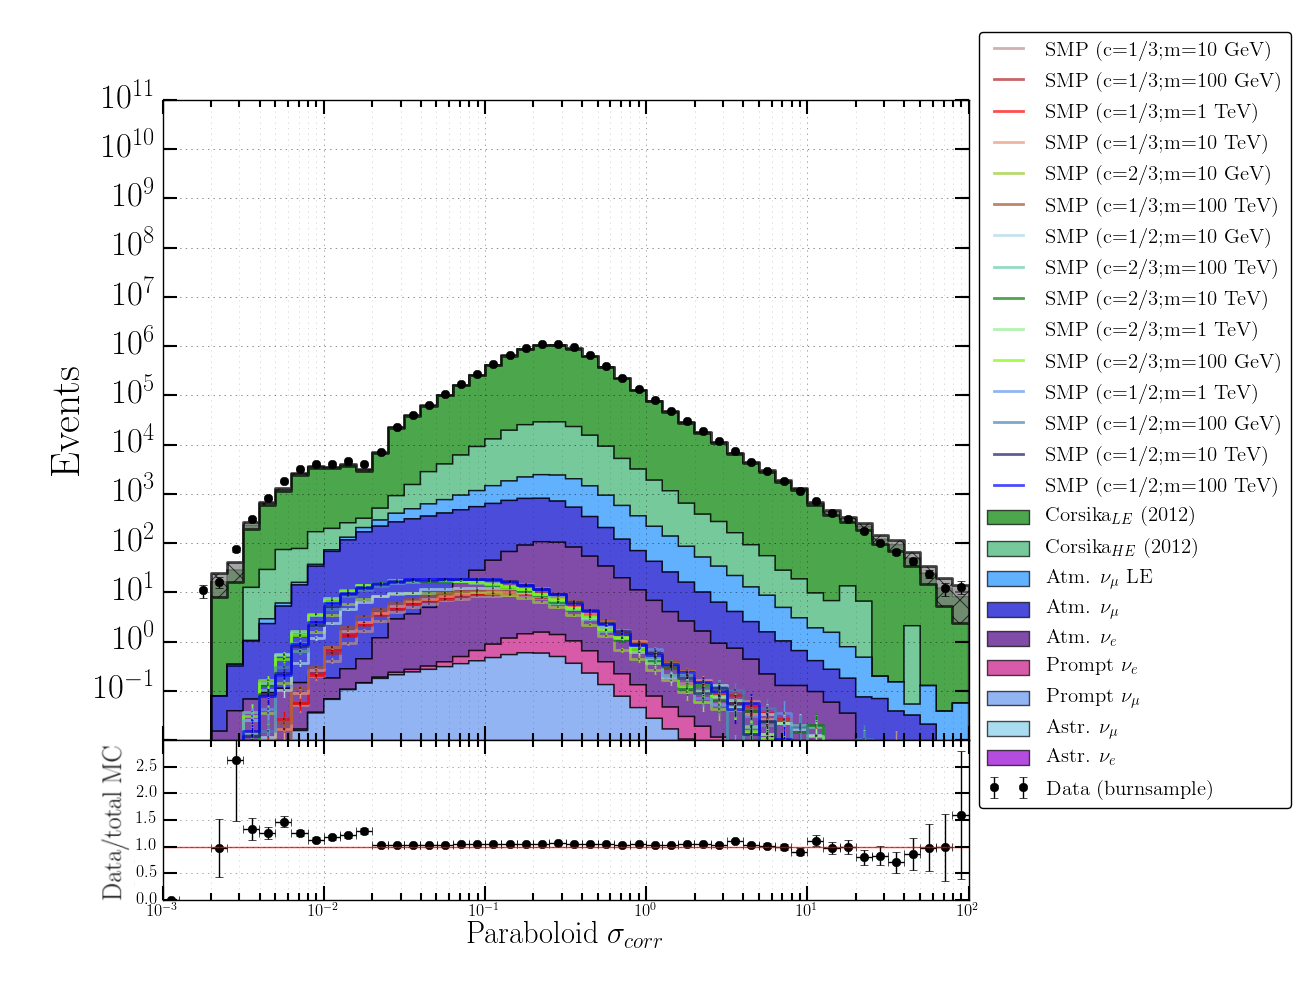
\includegraphics[width=0.9\textwidth]{chapter8/img/1D_stack_sigma_corr_paraboloid}
\caption{Distributions for the \texttt{Paraboloid} sigma.}
\label{fig:remainingvariablespara}
\end{figure}


\begin{figure}
\centering
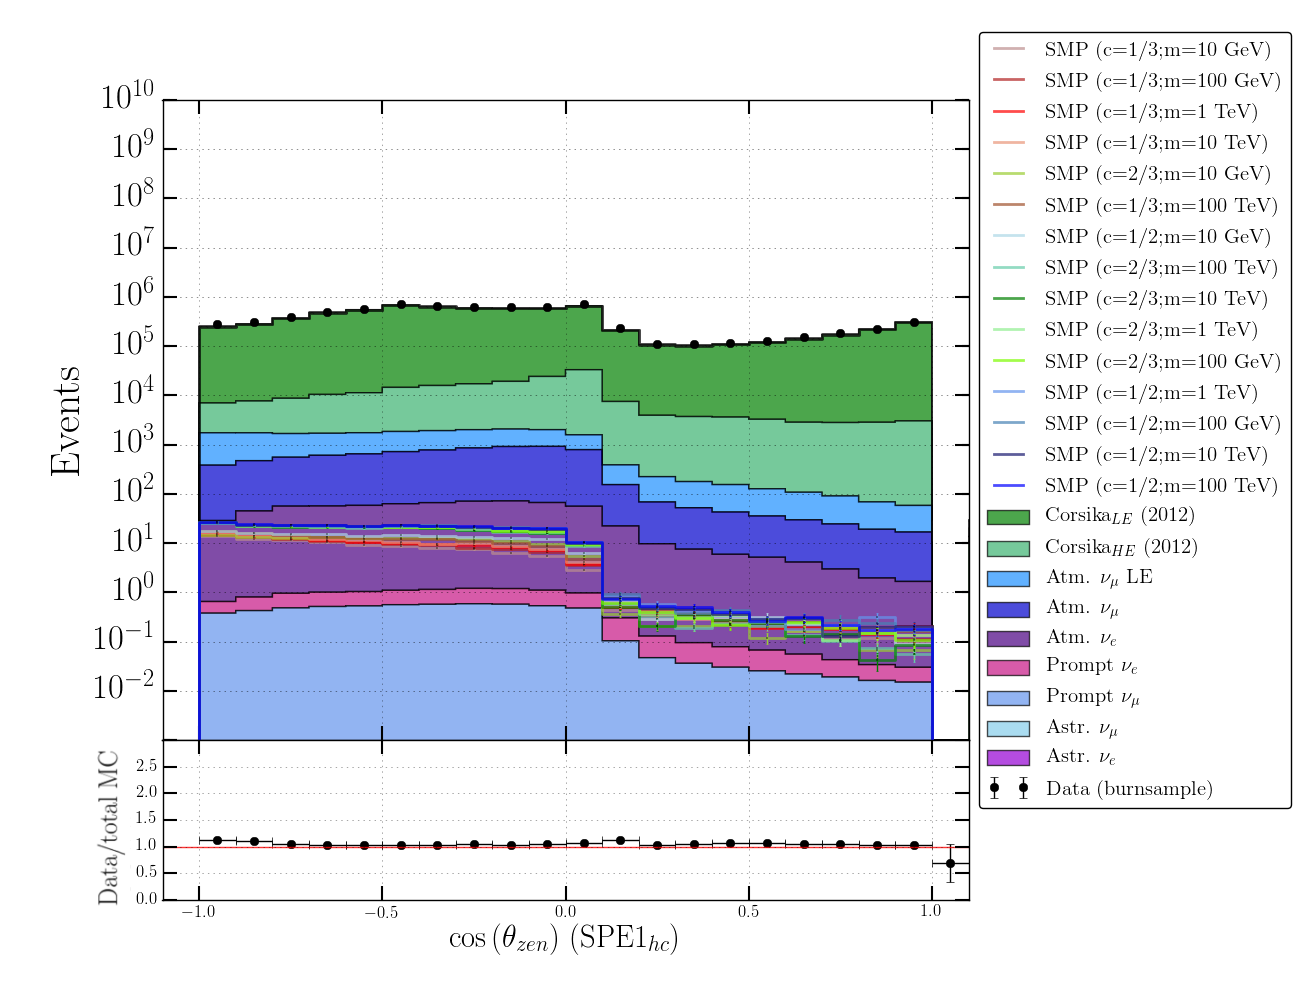
\includegraphics[width=0.9\textwidth]{chapter8/img/1D_stack_spefit1_hc_coszenith_foefelare}
\caption{Zenith distribution of the SPE reconstruction.}
\label{fig:remainingvariableszenith}
\end{figure}




\subsection{Variable selection}
The variables that are used in the BDT at Level 5 were selected by using the mRMR technique that was explained in Section \ref{sec:mrmr}. The 17 most important variables were used in the BDT. Less variables meant a lower performance while more variables did not show to add additional power in the BDT performance and meant more computational resources were necessary. In a BDT, one variable will be more important than another. Some variables have a much larger discrimination power than others. Therefore, an overview of all the variables used in Level 5 is shown in Table \ref{tab:mrmrimportance}. One BDT was used to show the relative importance (number from 0 to 1) of the variables. The importance is computed by counting the amount of split nodes using each
variable and weighing each count by the separation gain and by the overall weight of the tree in the forest. More information can be found in Ref. \cite{pybdturl}.

\textcolor{red}{DIRK ZEGGEN}

\begin{table}[]
\footnotesize
\caption{\textit{Left: }The 17 variables that are used in Level 5 are grouped per class. One BDT was used to show the relative importance (number from 0 to 1) of each variable. The order indicates the rank of which variable is most useful. \textit{Right: }The same variables shown in function of their rank.}
\label{tab:mrmrimportance}
\begin{tabular}{|l|r|c|c|}
\hline
\rowcolor[HTML]{F1A91E} 
Class & \multicolumn{1}{|c|}{Variable} & Order & \multicolumn{1}{l|}{\cellcolor[HTML]{F1A91E}Rel. importance} \\ \hline
 & ZMax & 2 & 0.109 \\ \cline{2-4} 
 & ZTravel & 3 & 0.106 \\ \cline{2-4} 
 & AvgDistToDom\_150 & 9 & 0.048 \\ \cline{2-4} 
 & TrackSeparation\_150 & 10 & 0.043 \\ \cline{2-4} 
 & TrackDistribution\_50 & 12 & 0.035 \\ \cline{2-4} 
 & TrackSeparation\_50 & 13 & 0.034 \\ \cline{2-4} 
 & EmptyHits\_100 & 16 & 0.027 \\ \cline{2-4} 
\multicolumn{1}{|c|}{\multirow{-8}{*}{\textbf{Commonvariables}}} & ZPattern & 17 & 0.016 \\ \hline
& RunsAboveMean & 4 & 0.105 \\ \cline{2-4} 
 & Mean\_dEdX & 5 & 0.074 \\ \cline{2-4} 
\multirow{-3}{*}{\textbf{Millipede}} & TrackLength\_60 & 11 & 0.039 \\ \hline
& NewLength\_150 & 1 & 0.132 \\ \cline{2-4} 
& NewLength\_all\_z & 6 & 0.059 \\ \cline{2-4} 
\multirow{-3}{*}{\textbf{New variables}} & SpeedRatio & 14 & 0.033 \\ \hline
 & LineFit\_Velocity & 7 & 0.055 \\ \cline{2-4} 
 & $\sigma_{\textrm{para}}$ & 8 & 0.051 \\ \cline{2-4} 
\multirow{-3}{*}{\textbf{Other variables}} & $\cos(\theta)_{\textrm{SPE}}$ & 15 & 0.033 \\ \hline
\end{tabular}
\begin{tabular}{|l|r|}
\hline
\rowcolor[HTML]{F1A91E} 
Order & Variable \\ \hline
\textbf{1} & NewLength\_150 \\ \hline
\textbf{2} & ZMax \\ \hline
\textbf{3} & ZTravel \\ \hline
\textbf{4} & RunsAboveMean \\ \hline
\textbf{5} & Mean\_dEdX \\ \hline
\textbf{6} & NewLength\_all\_z \\ \hline
\textbf{7} & LineFit\_Velocity \\ \hline
\textbf{8} & $\sigma_\textrm{para}$ \\ \hline
\textbf{9} & AvgDistToDom\_150 \\ \hline
\textbf{10} & TrackSeparation\_150 \\ \hline
\textbf{11} & TrackLength\_60 \\ \hline
\textbf{12} & TrackDistribution\_50 \\ \hline
\textbf{13} & TrackSeparation\_50 \\ \hline
\textbf{14} & SpeedRatio \\ \hline
\textbf{15} & $\cos(\theta)_\textrm{SPE}$ \\ \hline
\textbf{16} & EmptyHits\_100 \\ \hline
\textbf{17} & ZPattern \\ \hline
\end{tabular}
\end{table}


\section{Level 5}
The last part of the analysis makes use of the variables that were constructed and the 17 that were determined from the mRMR technique as the most powerful. First, the result from a single BDT is shown. Due to the lack of statistics in the final selection, the pull-validation method was used for a limit computation.

\subsection{BDT result}
The parameters that were used for BDT training (see Section \ref{sec:BDT}) are:
\vspace{2mm}
\begin{itemize}
\item Maximal depth: 2 (Figure \ref{fig:bdt})
\item Boosting $\beta$: 0.8 (Eq. \ref{eq:boostfactor})
\item Number of trees: 400 (Section \ref{subsec:boosting})
\item Pruning factor: 35 (Section \ref{subsub:pruning})
\end{itemize}
\vspace{2mm}
\noindent Training is done on 10\% of the available burn sample as it showed to have a better performance as opposed to training on background simulation. Training on the background samples showed a systematic disagreement between data and MC testing sets at the high BDT scores, probably due to limited statistics from the simulations at these high scores. The other 90\% of the burn sample is used for testing and is shown in the following plots. Testing on the MC data sets is also shown for the sake of completeness. Contribution of possible signal events, if they exist, in the data are minimal. Together with the very good data/MC agreement that is seen in the variables used, the training on data is a valid choice.

Also, it was chosen to select a (large) subsample of the Monte Carlo signal set instead of the complete set to train the BDT to give the best possible results. Some events in the signal MC will produce corner-clippers or leak-in events, which will often be mis-reconstructed. These events should not be used to train the BDT and are therefore removed in the training set. One can see in the variable distributions of Figures. \ref{fig:commonvariablesztravel} and \ref{fig:newvariablesnewlength} that there are minimal contributions of events with negative ZTravel and/or negative NewLength values. Upgoing tracks should give positive values for both and are therefore removed from the signal sample that is used to train the BDT\footnote{The final signal rate is computed from the full signal sample.}.\\

\noindent The result of one BDT can be seen in Figure \ref{fig:singlebdtrate} and we can draw several conclusions:
\vspace{2mm}
\begin{itemize}
\item Data and MC show a very good agreement.
\item The rate in background events is reduced by 4 to 5 orders of magnitude at a BDT score around 0.25.
\item At higher BDT scores, muons from low-energetic $\nu_\mu$ become a much more significant part of the total background than muons from air showers. This is mainly because the data used to train the decision tree mainly consists of atmospheric muons.
\item The signal used for training is more concentrated at higher scores, as expected. The total signal sample and the subset used for training overlap at scores higher than 0.1.
\item At the highest scores, where the signal dominates, it is clear that there is a lack of statistics in both CORSIKA simulations and the burn sample to draw sensible conclusions.
\end{itemize}
\vspace{2mm}
Additional checks can be found in Appendix \ref{ch:bdtchecks}.\\

\begin{figure}
\centering
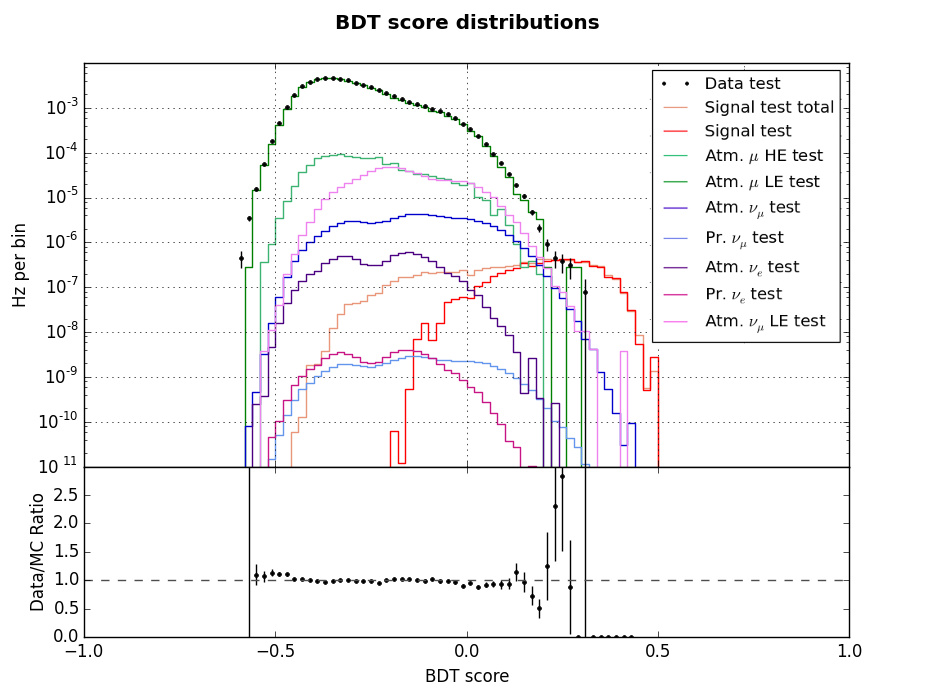
\includegraphics[width = 0.7\textwidth]{chapter8/img/dist_vs_bdt_result2_signal_m_100_charge1ovr2_better.png}
\caption{Rates of the various testing sample sets in function of the BDT score. Positive scores are more signal-like, whereas negative scores imply events that resemble the background the BDT was trained to recognize. The red curve corresponds to the subset of the signal that was used for training, while the gold curve corresponds to the total signal sample.}
\label{fig:singlebdtrate}
\end{figure}

\noindent The limited amount of statistics in the tail of the CORSIKA data sets proves challenging. There is a need for an order of magnitude more events, which is not feasible with the available resources. Other techniques, such as defining off-source or off-time regions \cite{1352676}, are not available for this search as we have assumed an isotropic flux that is not time-dependent.

\subsection{Pull-validation}
\label{subsec:pv}
Another way of dealing with limited statistics is by using re-sampling techniques. The method used here is called \textit{Pull-Validation}\footnote{The term \textit{pull} refers to the ``pulling'' of subsamples from a larger set, while \textit{validation} refers to the method being used to estimate uncertainties.} (PV) and was used several times before in the IceCube collaboration \cite{Aartsen:2016fep,Aartsen:2015exf,scheriauthesis}. It is comparable to bootstrapping and cross-validation (see Appendix \ref{ch:resampling}), but uses much smaller training samples. Smaller subsamples means more can be constructed uniquely and more subsamples lead to a larger variability that can be used as an estimator for the variability of the whole sample. As opposed to most bootstrapping and cross-validation methods, the resampling can be done without replacement\footnote{Selecting without replacement means that when an object is selected from a set, it is removed from the set so that it cannot be chosen twice or more.} because the samples are much smaller.

As can be seen in Figure \ref{fig:singlebdtrate}, there is a lack of statistics in the region of interest (at high BDT scores), mainly for the data burn sample and atmospheric muon simulations. Because we want to compute an upper limit from this distribution or set a discovery significance, a cut on the BDT score at a value that is higher than for example 0.30 does not result in a trustworthy background estimation. We cannot know from the distribution how the tail evolves into higher BDT scores. A cut on a single BDT implies a binary addition of an event to the final sensitivity: surviving the cut or not, and training the BDT on a slightly different training sample could result into a similar, but different BDT result. By using slightly different training samples, one is able to give an estimate about the tail of the background distributions in function of the BDT score.\\

\noindent Let us assume we have $N$ events making up a sample $S$. One BDT takes a subset $S_1$ and uses it as a training sample and using the remaining set for testing, $S_2$. 

\begin{equation}
k \cdot \left| S_1 \right| = \left| S_2 \right| \textrm{ with } S = S_1 \cup S_2 \textrm{ and } S_1 \cap S_2 = \oslash, 
\end{equation}
where $k$ refers to the order of missing events that is to be compensated. This factor cannot be made too small as the variability would diminish but cannot be made too large due to the limited size of $S$. Therefore, $k$ is set at 10. Because $S_2$ is sizeably larger, the testing sample will extend further than the training sample $S_1$ as can be seen in Figure \ref{fig:overtraining}. 

Pull-validation consists of repeating this procedure a number of times, $N_p$. For each iteration, the samples $S_1$ and $S_2$ are constructed from the sample $S$ and therefore, they consist of different events at each step. By combining the $N_p$ distributions, we can gain additional information from an event by obtaining the Probability Density Function (PDF) of an event in function of the BDT score. 

A single event will have one BDT score attributed per iteration and by reprocessing this $N_p$ times, while changing the training sample at each iteration, the variation of an event in function of the BDT score becomes visible and can be used as an estimation of the rate in the tails.\\

\noindent Each event gets an appropriate weight, the \textit{PV-weight} equal to

\begin{equation}
\label{eq:pullweight}
w_{PV} = \frac{\# \textrm{scores above cut threshold}}{N_p}.
\end{equation}

The number of pull-validation iterations, $N_p$, should be high enough to extract as much information as possible, but low enough so that the subsamples, which are 10\% of the total set chosen ad random each time, are still adding information in the variability of the BDT performance. Too many iterations would introduce correlation effects in the subsamples. Previous analyses indicated that $N_p = 200$ is good enough to fulfill these requirements \cite{Aartsen:2016fep,Aartsen:2015exf}. It is also used in this analysis. The result for an SMP with charge 1/2 and mass 100 GeV is shown in Figure \ref{fig:pullval} and shows the power of PV. Figure \ref{fig:betweenbins} illustrates how one bin in this histogram is constructed. For a certain BDT score range, a sample will have a rate that changes slightly when the BDT is trained with a different training sample. For example, one BDT estimates a rate of $x$ Hz for the signal between a BDT score if 0.30 and 0.31, whereas another BDT estimates a rate of $y$ Hz for the signal between these BDT scores. These rates, for all $N_p$ BDTs (divided by the average rate), are shown as a histogram in the figure. We can see that lower BDT scores imply more statistics and have a Gaussian-like distribution (left plot). For higher scores, the distribution resembles that of a log-normal or Poisson (right plot). The average rate is computed and used in the pull-validation histogram.\\
 
\begin{figure}
\centering
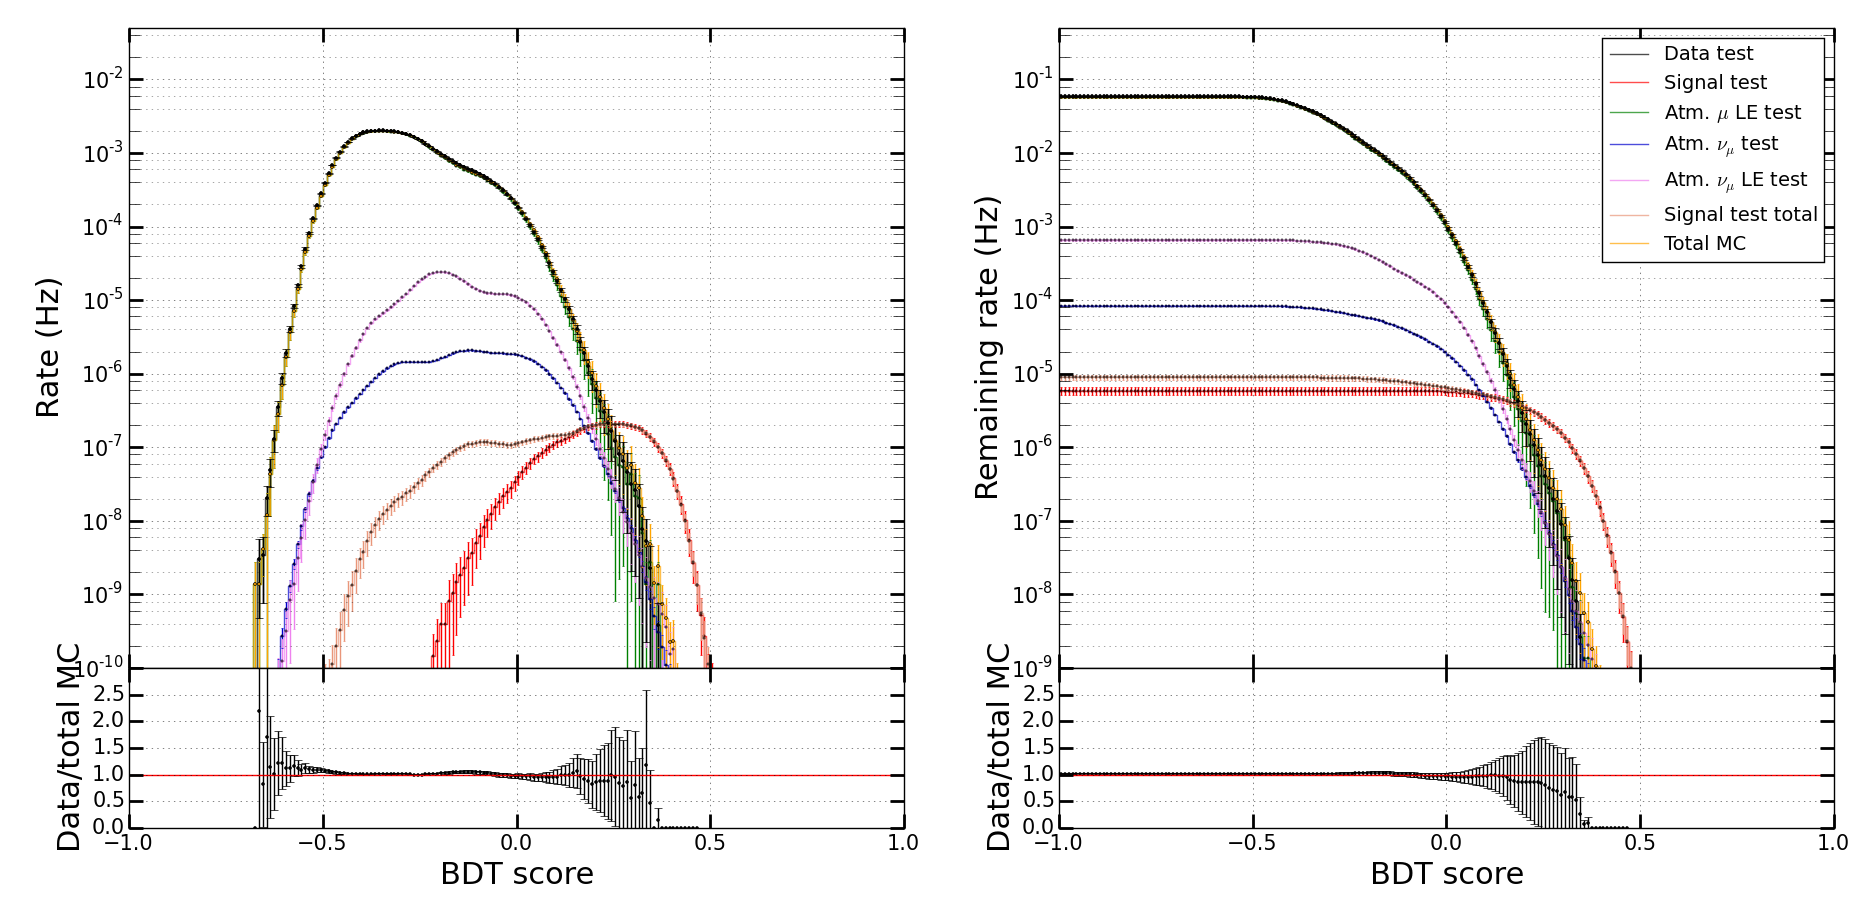
\includegraphics[width=\textwidth]{chapter8/img/pullval_result2_signal_m_100_charge1ovr2.png}
\caption{Result of the pull-validation method for an SMP with charge 1/2 and mass 100 GeV. Only the most prominent backgrounds are shown. \textit{Left: }rate in function of the BDT score. \textit{Right: }Cumulative rate to the right in function of the BDT score. The y-axis shows the remaining rate of a dataset when placing a cut at a certain BDT score. The weight of an event is given by Eq. \ref{eq:pullweight}.}
\label{fig:pullval}
\end{figure}

\begin{figure}
\centering
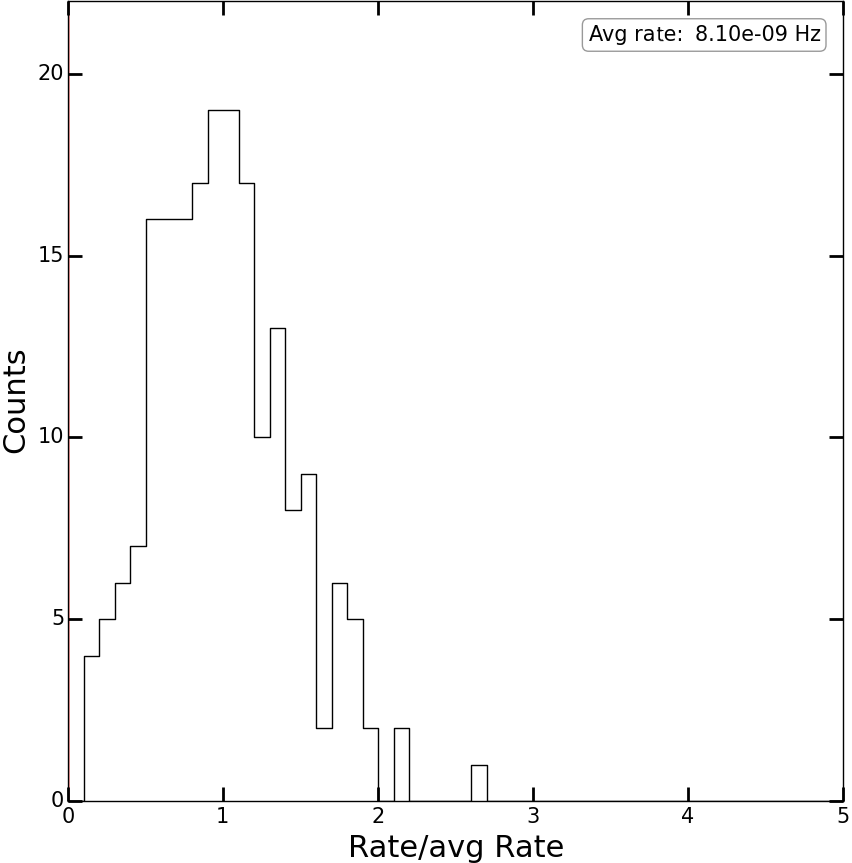
\includegraphics[width=0.49\textwidth]{chapter8/img/PMF_test_numu_atmos_bg_betweenbin_0p29_0p3_crop_typo.png}
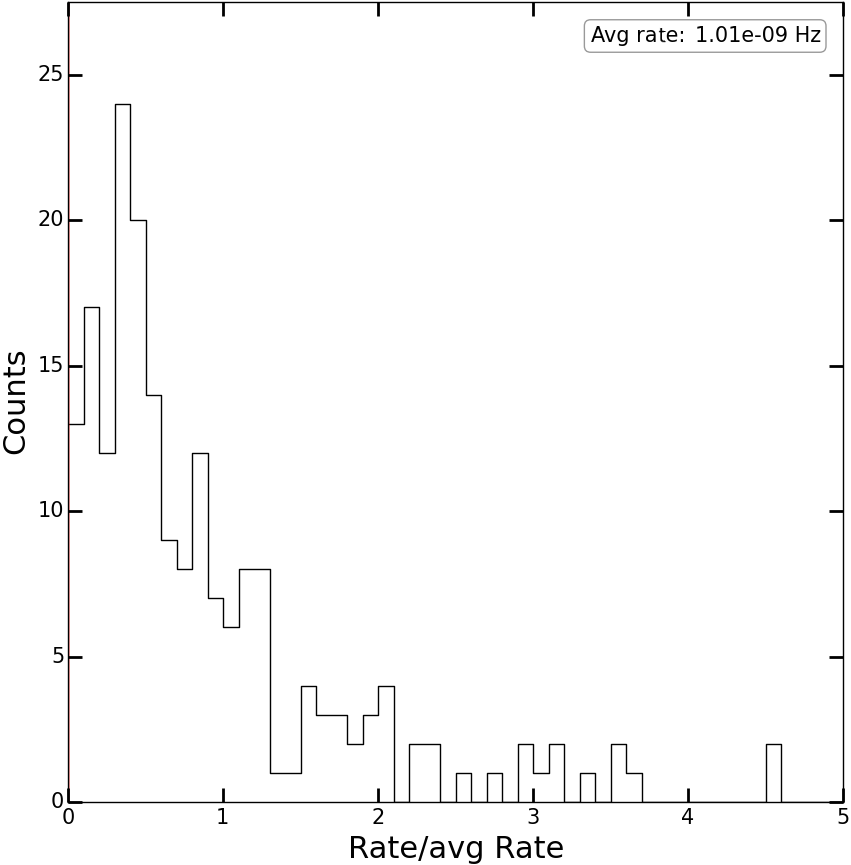
\includegraphics[width=0.49\textwidth]{chapter8/img/PMF_test_numu_atmos_bg_betweenbin_0p34_0p35_crop_typo.png}
\caption{Example of an uncertainty distribution of the atmospheric $\nu_\mu$ background with a BDT score between 0.29 and 0.3 (\textit{left}) and with a BDT score between 0.34 and 0.35 (\textit{right}).}
\label{fig:betweenbins}
\end{figure}


\subsection{Model Rejection Factor}
\label{subsec:mrf}
The question remains where we should place a cut in the BDT score for a significant signal discovery potential or upper limit computation. Since we do not know beforehand if the result will be a discovery or upper limit, the Feldman and Cousins method is used \cite{Feldman:1997qc}. In this analysis, we want to compute the 90\% confidence interval $\mu_{90} = (\mu_1, \mu_2)$, which is a function of the number of observed events, $n_\textrm{obs}$, and of the number of expected background evens, $n_\textrm{b}$

\begin{equation}
\mu_{90} \left(n_\textrm{obs},n_\textrm{b}\right).
\end{equation}

\noindent If we assume that the expected number of signal events is $n_\textrm{s}$, then the 90\% confidence upper limit on the signal flux is

\begin{equation}
\label{eq:flux}
\Phi_{90\%}\left(n_\textrm{obs},n_\textrm{b},n_\textrm{s}\right) = \Phi \cdot  \frac{\mu_{90}\left(n_\textrm{obs},n_\textrm{b}\right)}{n_\textrm{s}},
\end{equation}

\noindent where $\Phi$ is the assumed signal flux of $10^{-14}$ cm$^{-2}$ sr$^{-1}$ s$^{-1}$. It is important to mention that $n_\textrm{s}$ and $\Phi$ scale linearly, making the UL \textit{independent} of the assumed absolute flux. Unfortunately, an UL can only be computed once the number of observed events is known. The best \textit{expected} UL could be computed by assuming that the number of observed events is equal to the expected number of events from the MC background. Setting $n_\textrm{obs}$ equal to $n_\textrm{b}$ is, however, not a good approach for analyses that have small sample sets at the final level. For example, say one expects 2.5 background events with a 1$\sigma$ error of 2.1. If, after unblinding, one finds 0, 1, 2, 3, 4, or 5 events in data, this would be considered as consistent with the expected background. The 90\% Feldman-Cousins UL are, however, drastically different: $\mu_{90}(0,2.5) = 1.18, \ \mu_{90}(5,2.5) = 7.49$. Which is more than a factor of 6 difference! Do we simply take the mean of these two numbers?.

A better way is to assume that the number of observed events is the mean of a Poissonian distribution and we compute the \textit{average upper limit} by summing over all the expected upper limits, weighted by their Poisson probability of occurring \cite{Hill:2002nv}

\begin{equation}
\begin{split}
\overline{\mu}_{90}(n_\textrm{b}) &= \sum^{\infty}_{n_\textrm{obs}=0} \mu_{90}\left(n_\textrm{obs},n_\textrm{b}\right) \cdot \textrm{Poiss}\left(n_\textrm{obs},n_\textrm{b}\right)\\
&= \sum^{\infty}_{n_\textrm{obs}=0} \mu_{90}\left(n_\textrm{obs},n_\textrm{b}\right) \cdot \frac{\left(n_\textrm{b}\right)^{n_\textrm{obs}}}{\left(n_\textrm{obs}\right)!} \exp\left(-n_\textrm{b}\right)
\end{split}
\end{equation}

\noindent The \textit{Model Rejection Factor} (MRF) is defined as 

\begin{equation}
\textrm{MRF}\left(n_\textrm{b}, n_\textrm{s}\right) =  \frac{\overline{\mu}_{90}\left(n_\textrm{b}\right)}{n_s}.
\end{equation}
\noindent Comparing this with Eq. \ref{eq:flux}, we can see that minimizing this factor corresponds to the strongest possible constraint on the expected signal flux. Because in each bin in Figure \ref{fig:pullval} both the number of expected signal events and background events are known, the MRF can be computed in function of the BDT score. This is shown in Figure \ref{fig:mrf} for an SMP with charge 1/2 and mass 100 GeV. In the figure, all samples are normalized to a livetime of 1723 days ($\approx$4 years and 262 days). The value of the minimal MRF is shown, together with the corresponding BDT bin. The lowest value of the bin was chosen as the BDT cut for each signal sample. Also, we present the number of expected MC signal events, MC backgrounds, and data (where the burn sample is scaled to the total live time). The uncertainties correspond to statistical uncertainties only. A fake unblinding is presented where we show the expected UL, together with the UL if we would use the burn sample that has more statistics due to the PV method.

After pull-validation, there are enough statistics for a proper MRF computation (purple). The offset of data from MC is a common feature in PV and is accounted for in the systematic uncertainties.

The MRF gives a numerical indication of where we find an optimal trade-off of expected signal and background events. At very high scores, there are less background events expected, but also less of the signal while at lower scores both have higher expectancies.\\

\begin{figure}
\centering
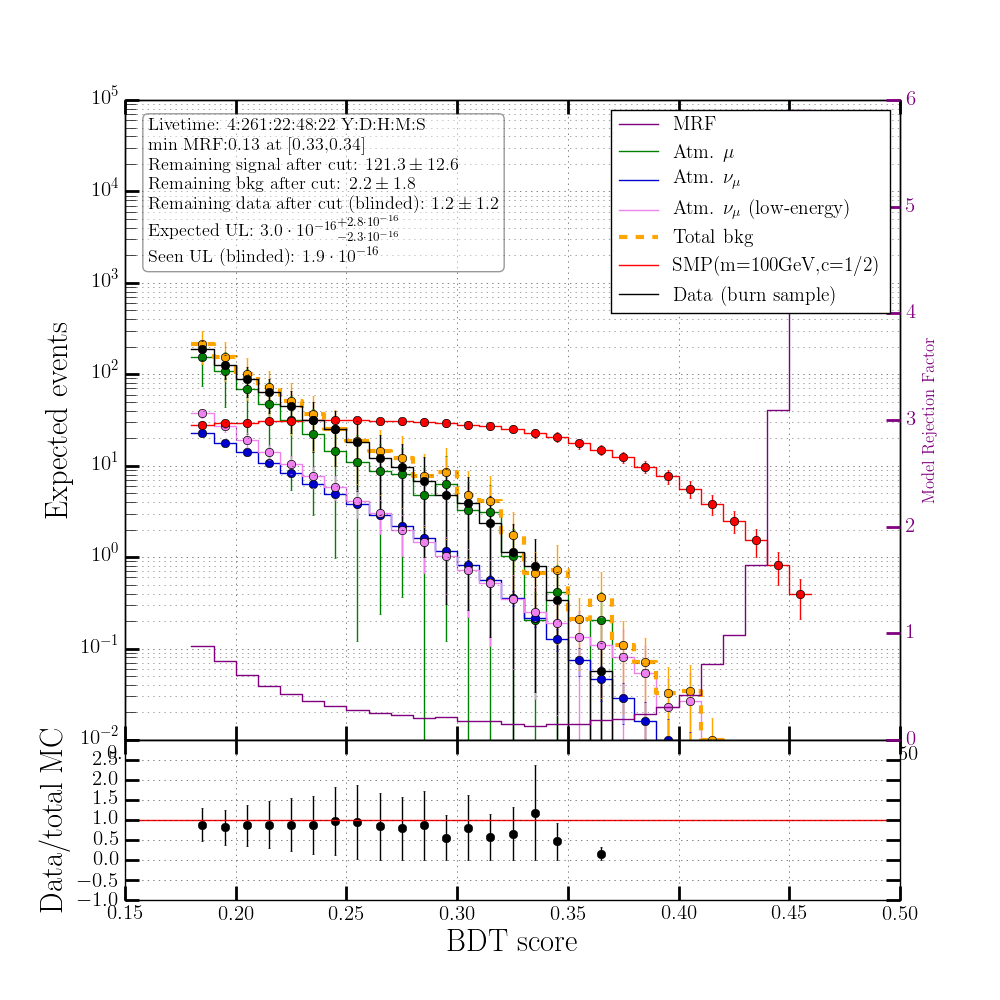
\includegraphics[width=0.9\textwidth]{chapter8/img/ModelRejectionFactor_percentile_0p9_signal_m_100_ch_1ovr2_noSYST.png}
\caption{Zoomed in version of Figure \ref{fig:pullval}, focused on higher BDT scores, again for an SMP with charge 1/2 and mass 100 GeV. Only the most prominent backgrounds are shown. The expected rate is shown on the left vertical axis, while the MRF score can be obtained from the right vertical axis. Only statistical uncertainties are shown as error bars.}
\label{fig:mrf}
\end{figure}

\noindent The BDT score where the MRF is minimized was chosen as the final cut; this is the cut that will probably give the most stringent upper limit or best value for an observation. It's possible that another cut yields more stringent upper limits, but this cannot be known before unblinding the total data set. This should not be done to leave the analyzer unbiased. Therefore, the MRF method uses a Poissonian weighting, which yields us the most probable stringent upper limit. The results can be found in Table \ref{tab:expectedresults}.

\begin{table}[]
\centering
\renewcommand{\arraystretch}{1.5}
\caption{Expected number of signal and background events for 5 years of data (see Section \ref{sec:results}), errors are statistical only. The signal is normalized to a flux of $10^{-14} \ \textrm{cm}^{-2} \textrm{s}^{-1} \textrm{sr}^{-1}$. The optimal BDT cut value from the MRF minimization is shown together with the expected upper limit and the statistical error.}
\label{tab:expectedresults}
\resizebox{\textwidth}{!}{%
\begin{tabular}{|l |c|c|c|c|c|}
\hline
\cellcolor[HTML]{F1A91E}Mass & \cellcolor[HTML]{F1A91E}Charge & \cellcolor[HTML]{F1A91E}\begin{tabular}[c]{@{}c@{}}Remaining MC signal events\\ per 1723 days\end{tabular} & \cellcolor[HTML]{F1A91E}\begin{tabular}[c]{@{}c@{}}Remaining MC background events\\ per 1723 days\end{tabular} & \cellcolor[HTML]{F1A91E}\begin{tabular}[c]{@{}c@{}}$\overline{\mu}_{90}\left(\textrm{cm}^{-2} \textrm{s}^{-1} \textrm{sr}^{-1}\right)$ \\$\times 10^{{-16}} $\end{tabular}& \cellcolor[HTML]{F1A91E}BDT cut value \\ \hline
\textbf{10 GeV} &  & $73.2\pm7.7$ & $2.2\pm1.6$ & $5.0^{ +2.9 }_{ -3.8 }$ & 0.32 \\ \cline{3-6} 
\textbf{100 GeV} &  & $121.3\pm12.6$ & $2.2\pm1.8$ & $3.0^{ +2.8}_{ -2.3}$ & 0.33 \\ \cline{3-6}
\textbf{1 TeV} &  & $90.7\pm9.6$ & $0.8\pm0.6$ & $1.9^{ +2.5}_{ -0.18}$ & 0.35 \\ \cline{3-6}
\textbf{10 TeV} &  & $127.8\pm11.0$ & $1.8\pm1.1$ & $2.1^{ +1.4 }_{ -1.2}$ & 0.34 \\ \cline{3-6}
\textbf{100 TeV} & \multirow{-5}{*}{1/2} & $107.7\pm9.7$ & $2.2\pm1.3$ & $ 3.4^{ +1.9}_{ -2.6 }$ & 0.34 \\ \hline
\textbf{10 GeV} &  & $45.3\pm5.2$ & $2.2\pm1.9$ & $8.2^{ +7.7 }_{ -6.2 }$ & 0.32 \\ \cline{3-6}
\textbf{100 GeV} &  & $60.5\pm4.1$ & $2.4\pm1.9$ & $ 5.9^{ +5.1 }_{ -4.5}$ & 0.35 \\ \cline{3-6}
\textbf{1 TeV} &  & $64.0\pm5.6$ & $3.1\pm2.7$ & $6.7^{ +5.0 }_{ -5.4}$ & 0.32 \\ \cline{3-6}
\textbf{10 TeV} &  & $57.6\pm4.9$ & $1.2\pm1.0$ & $5.5^{ +3.4}_{ -3.1}$ & 0.34 \\ \cline{3-6}
\textbf{100 TeV} & \multirow{-5}{*}{1/3} & $79.7\pm5.9$ & $2.2\pm1.5$ & $ 4.6^{ +2.4}_{ -3.5}$ & 0.34 \\ \hline
\textbf{10 GeV} &  & $40.4\pm4.5$ & $9.6\pm3.7$ & $14.2^{ +15.1}_{ -10.4}$ & 0.29 \\ \cline{3-6}
\textbf{100 GeV} &  & $71.5\pm7.5$ & $5.0\pm1.4$ & $5.1^{ +5.1}_{ -1.5}$ & 0.30 \\ \cline{3-6}
\textbf{1 TeV} &  & $79.3\pm7.7$ & $7.2\pm2.1$ & $6.7^{ +4.6 }_{ -3.1}$ & 0.30 \\ \cline{3-6}
\textbf{10 TeV} &  & $74.4\pm7.9$ & $7.9\pm2.2$ & $6.3^{ +6.7}_{ -3.1}$ & 0.29 \\ \cline{3-6}
\textbf{100 TeV} & \multirow{-5}{*}{2/3} & $59.0\pm6.0$ & $5.7\pm1.6$ & ${ 7.4}^{ +5.6}_{ -2.7}$ & 0.30 \\ \hline
\end{tabular}%
}
\end{table}


\subsection{Systematic uncertainties}
There are four types of uncertainties that are assumed in the result of this analysis, which are listed below

\vspace{2mm}
\begin{enumerate}
\item \textbf{Statistical:} Limited statistics in the final event sample in both the expected signal and background events lead to uncertainties. We assume that the variance of this number follows a Poisson distribution where the statistical uncertainty on a rate is defined as the square root of the rate. The statistical uncertainties can be seen in Table \ref{tab:expectedresults}.
\item \textbf{Detector: } Detector simulations assume certain properties of the optical modules and the ice (see Chapter \ref{ch:icecube}), which can differ from true values or are oversimplistic. Therefore, the following detector uncertainties are assumed:
\vspace{2mm}
\begin{itemize}
\item DOM efficiency +10\%
\item DOM efficiency -10\%
\item Ice absorption +10\%
\item Ice scattering +10\%
\item Ice absorption and scattering -7.1\%
\end{itemize}
\vspace{2mm}
The DOM efficiencies originate from uncertainties in the DOM calibrations, whereas the ice absorption and scattering uncertainties are conservative estimates, determined by the collaboration. Therefore, specialized simulation data sets that include these uncertainties were developed and are shown in Table \ref{tab:systematics}. Because of the limited statistics in the systematic background sample sets, these detector uncertainties are investigated before the BDT training at Level 4. The effects on the signal were investigated after BDT cuts of 0.30 for charge 2/3 particles and 0.32 for charge 1/3 and 1/2 particles. There were no significant differences found for different masses and these are therefore not specified. Results are shown in Table \ref{tab:detectoruncertainties}.
\item \textbf{Flux: }The models that were used in flux normalizations are not set in stone. Therefore, variations to the flux were assumed to determine the possible discrepancies.
\begin{itemize}
\item \textit{SMP flux}: As there is no clear production model or clear possible origin of these anomalous charged particles, the signal flux is assumed to range between $E^{-1}$ and $E^{-3}$. 
\item \textit{Atmospheric $\mu$ flux: }We look at the difference between the GaisserH3a \cite{Gaisser:2013bla} and GaisserH4a \cite{Gaisser:2011cc} models.
\item \textit{Atmospheric $\nu_\mu$ flux: }We look at the difference between the Bartol \cite{PhysRevD.70.023006} and Honda2006 \cite{Honda:2006qj} models.
\end{itemize}
Similar to the detector uncertainties, the effects were computed at Level 4 for background data sets and at BDT cuts of 0.32, 0.32 and 0.30 for particles with charges 1/2, 1/3 and 2/3 respectively. The data sets used for detector and flux uncertainties are shown in Table \ref{tab:systematics}. Results are shown in Table \ref{tab:detectoruncertainties}. Because these numbers were computed from relatively small sample sets\footnote{Data sets that were constructed for systematic uncertainty have much less statistics than the nominal ones.}, there are uncertainties on these numbers as well. For example, the scattering +10 \% uncertainties have an error of around $(19.3 \pm 14)$ \%, $(3 \pm 10)$\%, and $(3.4 \pm 15)$\%.

\begin{table}[]
\footnotesize
\centering
\caption{Overview of the data sets used for systematic uncertainties. Polyg(onato) follows from Ref. \cite{Hoerandel:2002yg}, GaisserH4a from Ref. \cite{Gaisser:2011cc} and Bartol from Ref. \cite{PhysRevD.70.023006}.}
\label{tab:systematics}
\resizebox{\textwidth}{!}{%
\begin{tabular}{|l|c|c|c|c|c|c|r|}
\hline
\rowcolor[HTML]{F1A91E} 
Generator & Type & Range {[}GeV{]} & Sim. $\gamma$ & Weighted $\gamma$ & Ice & Dataset & Syst. Eff. \\ \hline
\textbf{CORS.} & Hoerandel & $600 - 10^5$ & Polyg. & GaisserH3a & SpiceLea & 11527 & DOM eff. -10\% \\ \hline
\textbf{CORS.} & Hoerandel & $600 - 10^{11}$ & Polyg. & GaisserH3a & SpiceLea & 11526 & DOM eff. +10\% \\ \hline
 &  &  &  &  &  &  & Abs. +10\% \\ \cline{8-8} 
 &  &  &  &  &  &  & Scat. +10\% \\ \cline{8-8} 
\multirow{-3}{*}{\textbf{CORS.}} & \multirow{-3}{*}{5-comp.} & \multirow{-3}{*}{$600 - 10^{11}$} & \multirow{-3}{*}{2.6} & \multirow{-3}{*}{GaisserH3a} & \multirow{-3}{*}{SpiceLea} & \multirow{-3}{*}{12388} & \multicolumn{1}{l|}{Abs./Scat. -7.1\%} \\ \hline
\textbf{CORS.} & \multicolumn{3}{c|}{All data sets from Table \ref{tab:datasets}} & GaisserH4a & SpiceLea & Table \ref{tab:datasets} & GaisserH4a \\ \hline
\textbf{NuGen} & $\nu_\mu$ & $100 - 10^8$ & 2 & Bartol (syst.) & SpiceLea & 11029 & Bartol flux \\ \hline
 &  &  &  &  &  &  & DOM eff. +10\% \\
 &  &  &  &  &  &  & DOM eff. -10\% \\
 &  &  &  &  &  &  & Abs. +10\% \\
 &  &  &  &  &  &  & Scat. +10\% \\
 &  &  &  &  &  &  & Abs./Scat. -7.1\% \\
\multirow{-6}{*}{\textbf{NuGen}} & \multirow{-6}{*}{$\nu_\mu$} & \multirow{-6}{*}{$100 - 10^7$} & \multirow{-6}{*}{2} & \multirow{-6}{*}{\begin{tabular}[c]{@{}c@{}}Honda2006\\ \\ + Bartol (syst.)\end{tabular}} & \multirow{-6}{*}{SpiceLea} & \multirow{-6}{*}{11883} & Bartol flux \\ \hline
 &  &  &  &  &  &  & DOM eff. +10\% \\
 &  &  &  &  &  &  & DOM eff. -10\% \\
 &  &  &  &  &  &  & Abs./Scat. -7.1\% \\
\multirow{-4}{*}{\textbf{NuGen}} & \multirow{-4}{*}{$\nu_\mu$} & \multirow{-4}{*}{$100 - 10^8$} & \multirow{-4}{*}{2} & \multirow{-4}{*}{\begin{tabular}[c]{@{}c@{}}Honda2006\\ \\ + Bartol (syst.)\end{tabular}} & \multirow{-4}{*}{SpiceLea} & \multirow{-4}{*}{12346} & Bartol flux \\ \hline
\end{tabular}%
}
\end{table}

\item \textbf{Pull-validation: }As will be explained in Section \ref{sec:results}, only one BDT is used for the final event rate. Pull-validation offers us a way to get more statistics but choosing one BDT for the full data sample and comparing the data rate to the mean of a fluctuating pool of expected background events gives rise to a large uncertainty. It was found that this uncertainty is highly dominant.

\hspace{3mm} For each mass point I have looked at the minimal and maximal offsets between the 200 BDT outputs. As the signal distributions again had enough statistics at higher BDT scores, cuts at values of 0.32, 0.32 and 0.30 for particles with charges 1/2, 1/3 and 2/3 were chosen respectively. Background distributions showed unrealistic large fluctuations in the tails due to very low statistics and single events with high or low weights. Therefore, the BDT cuts were lowered to 0.25 for the backgrounds. The largest discrepancy between the average and the minimum and maximum is set as the uncertainty as a conservative choice. An example is shown in Figure \ref{fig:pvuncertainty}. The results can be found in Table \ref{tab:pvuncertainties}.
\end{enumerate}
\vspace{2mm}

\begin{table}[]
\centering
\caption{Results for the absolute numbers of the detector and flux uncertainties.}
\label{tab:detectoruncertainties}
\resizebox{\textwidth}{!} & 30.9\% & 2.9\% & 7.6\% & 5.2\% & 3.6\% \\ \hline
\textbf{DOM eff. -10\%} & 26.7\% & 29.4\% & 3.5\% & 16.7\% & 0.8\% \\ \hline
\textbf{Absorption +10\%} & 23.9\% & 2.2\% & 22.7\% & 18.5\% & 38.3\% \\ \hline
\textbf{Scattering +10\%} & 3.6\% & 2.9\% & 19.3\% & 3\% & 3.4\% \\ \hline
\textbf{Abs./Scat -7.1\%} & 17.7\% & 5.8\% & 18.7\% & 6.4\% & 12.1\% \\ \hline
\textbf{Flux} & 0.35\% & 15.28\% & 1.7\% & 3\% & 11.8\% \\ \hline \hline
\textbf{Total} & 50.7\% & 33.9\% & 36.2\% & 26.6\% & 42.5\% \\ \hline
\end{tabular}%
}
\end{table}

\begin{figure}
\centering
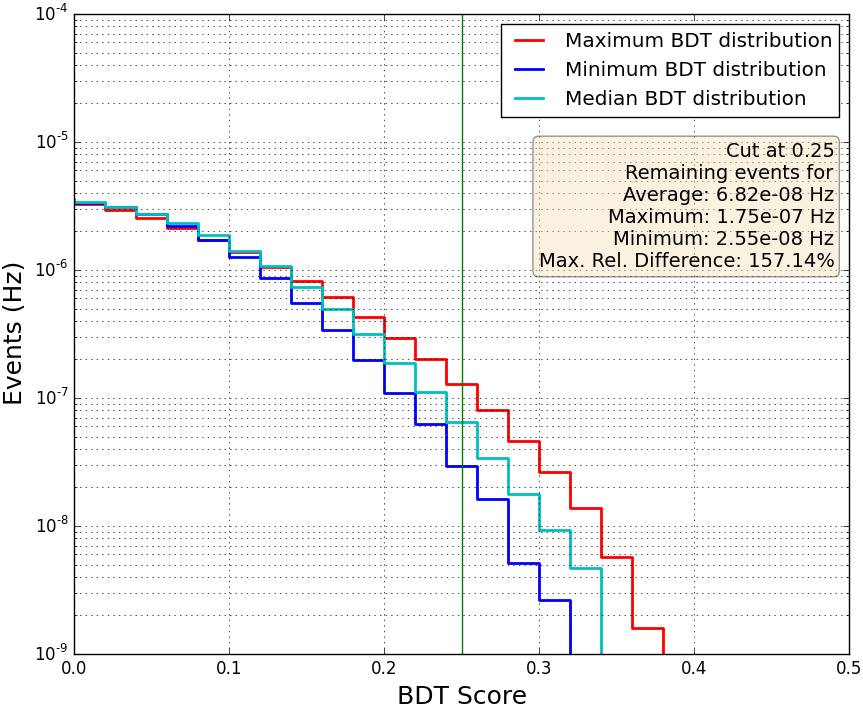
\includegraphics[width=0.49\textwidth]{chapter8/img/PVUncertainty_sig_m_100_c_1ovr2_BDTCUT0p25_test_numu_atmos_bg.png}
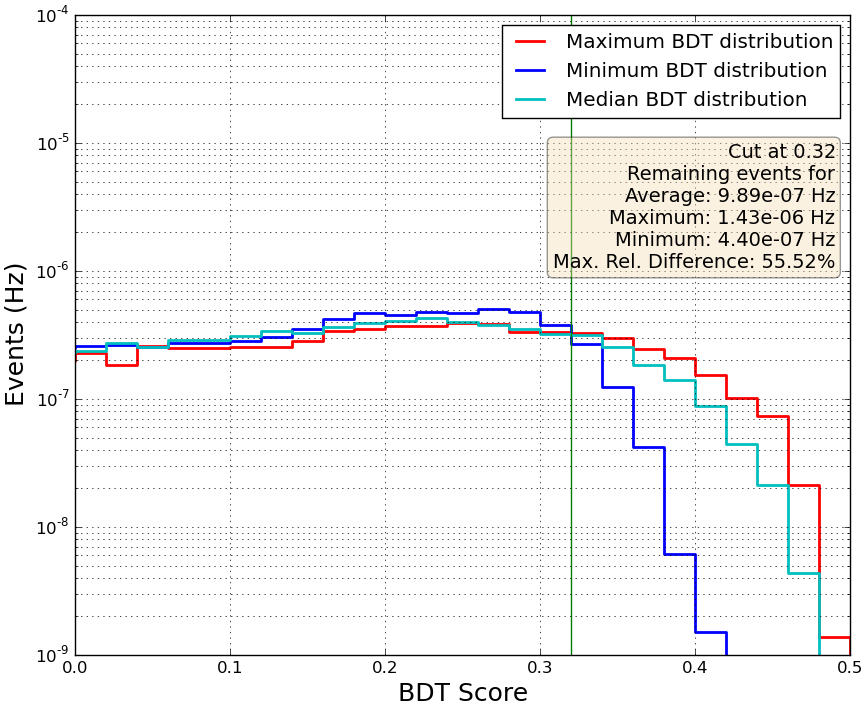
\includegraphics[width=0.49\textwidth]{chapter8/img/PVUncertainty_sig_m_100_c_1ovr2_BDTCUT0p32_total_test_sig}
\caption{\textit{Left: }Illustration how the pull-validation systematic error is computed. Here, the maximum rate, the median and minimum rates from 200 BDT score distributions are shown. \textit{Right: }Similar comparison of BDT score distributions for an SMP with a charge 1/2 and mass 100 GeV.}
\label{fig:pvuncertainty}
\end{figure}

\begin{table}[]
\centering
\caption{Results for the pull-validation uncertainties}
\label{tab:pvuncertainties}
\begin{tabular}{|l |c|c|c|c|}
\hline
\cellcolor[HTML]{F1A91E}Mass & \cellcolor[HTML]{F1A91E}Charge & \cellcolor[HTML]{F1A91E}Atm. $\mu$ & \cellcolor[HTML]{F1A91E}Atm. $\nu_\mu$ & \cellcolor[HTML]{F1A91E}SMP \\ \hline
\textbf{10 GeV} &  & 66.4\% & 216.1\% & 59.8\% \\ \cline{3-5}
\textbf{100 GeV} &  & 136.3\% & 157.1\% & 55.5\% \\ \cline{3-5}
\textbf{1 TeV} &  & 159.8\% & 136.3\% & 42.1\% \\ \cline{3-5}
\textbf{10 TeV} &  & 211.6\% & 73.7\% & 36.7\% \\ \cline{3-5}
\textbf{100 TeV} & \multirow{-5}{*}{1/2} & 218.4\% & 135.4\% & 52.5\% \\ \hline
\textbf{10 GeV} & & 142\% & 176.7 & 39.6\% \\ \cline{3-5}
\textbf{100 GeV} & & 174.8\% & 225.6\% & 32.9\% \\ \cline{3-5}
\textbf{1 TeV} & & 108.3\% & 167\% & 40.9\% \\ \cline{3-5}
\textbf{10 TeV} & & 190.3\% & 150\% & 40.8\% \\\cline{3-5}
\textbf{100 TeV} & \multirow{-5}{*}{1/3} & 223.6\% & 96.8\% & 35.6\% \\ \hline
\textbf{10 GeV} & & 63.8\% & 103.6\% & 54.8\% \\ \cline{3-5}
\textbf{100 GeV} & & 58.7\% & 88.9\% & 52.5\% \\\cline{3-5}
\textbf{1 TeV} & & 65.4\% & 72.5\% & 61.9\% \\ \cline{3-5}
\textbf{10 TeV} & & 10\% & 104.2\% & 72.1\% \\ \cline{3-5}
\textbf{100 TeV} & \multirow{-5}{*}{2/3} & 51.5\% & 83.4\% & 43.6\% \\ \hline
\end{tabular}
\end{table}

\noindent The final systematic uncertainty is obtained by summing the individual uncertainties in quadrature.

\paragraph{Implementing the uncertainties in the upper limit}
Using Eq. \ref{eq:flux}, we are able to determine an upper limit in the scenario where we cannot claim detection. Because there are large uncertainties in both the background and signal rates, these uncertainties are included in the computation of the limit. The \textit{observed} limit will be weighted with an uncertainty probability. Additionally, we will also show systematic uncertainty bands as can be seen in Figures \ref{fig:moneyplot1} to \ref{fig:moneyplot4}. 

Gaussian distributions with large uncertainties overlap with negative rates, which are not physical (e.g. an expected rate of 2 events with a 150\% uncertainty would yield a range of $\left[-1,+5\right]$. A rate of -1 is unphysical.), therefore we assume that the uncertainties follow a truncated normal distribution 

\begin{equation}
\label{eq:finalUL}
\Phi(n_\textrm{obs}, n_\textrm{bkg}, \sigma_{\textrm{bkg}}, n_\textrm{s}, \sigma_{\textrm{s}} )_{90\%} = \Phi \cdot \frac{\sum^\infty_{n'_{bkg}} \left[ \mu_{90}\left(n_\textrm{obs},n'_\textrm{bkg} \right) \cdot P_\textrm{unc} \left(n'_\textrm{bkg}|n_\textrm{bkg},\sigma_{\textrm{bkg}}\right) \right]}{\sum^\infty_{n'_s = 0} n'_s \cdot P_\textrm{unc}\left(n'_\textrm{s} | n_\textrm{s}, \sigma_{\textrm{s}}\right)},
\end{equation}
where

\begin{equation}
\label{eq:pdfUnc}
P_\textrm{unc}\left(n|\lambda, \sigma \right) = \int^\infty_{-\lambda} \frac{\left(\lambda + x\right)^n e^{-\lambda-x}}{n!} \cdot w(x,\sigma)dx,
\end{equation}
with $w(x,\sigma)$ a normal distribution with mean 0 and variance $\sigma^2$. An example of two distributions for both the signal and background are shown in Figure \ref{fig:pvuncertaintieswidth}. We can see that large rates with large uncertainties lead to Gaussian distributions (right figure). If a part of the distribution extends to negative rates, the formula (Eq. \ref{eq:pdfUnc}) removes these negative rates and scales the probabilities accordingly. Therefore, the total integrated probability is always one. Very low rates with relatively large uncertainties give much larger probabilities to very low number of events (left figure). Negative numbers are again removed.

\begin{figure}
\centering
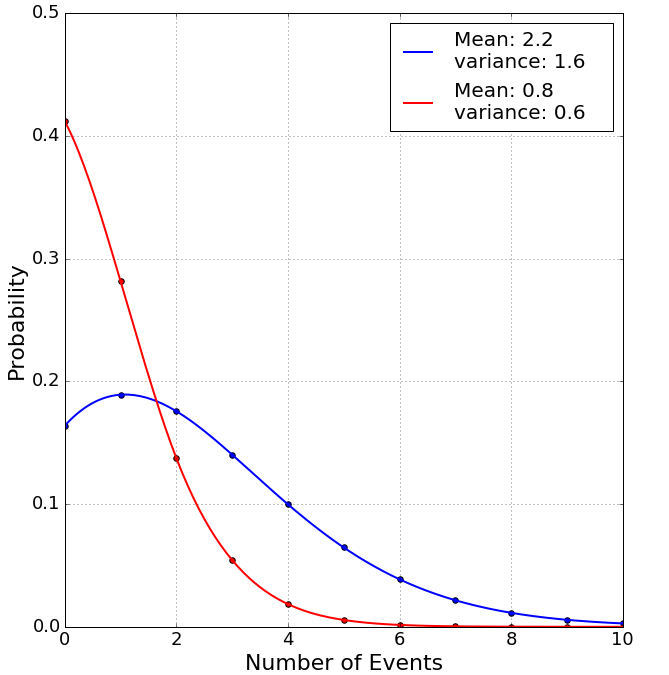
\includegraphics[width=0.49\textwidth]{chapter8/img/PVuncertainty_asweights_background.png}
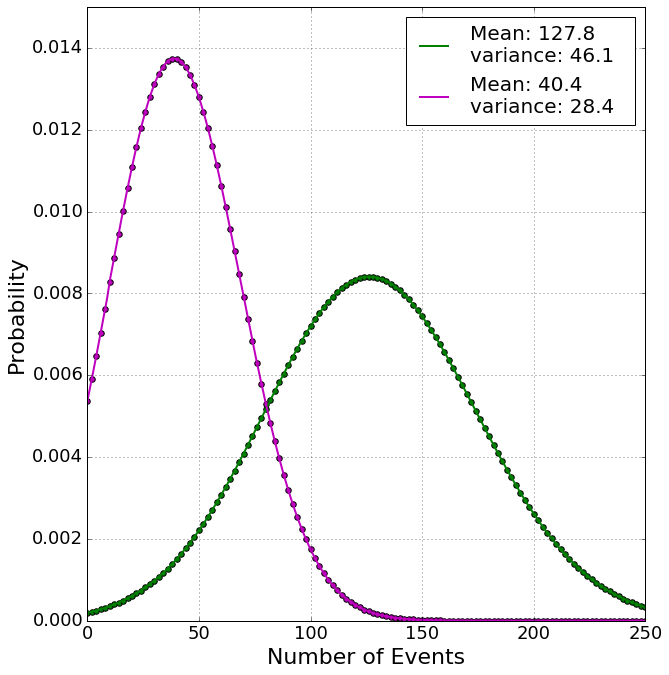
\includegraphics[width=0.49\textwidth]{chapter8/img/PVuncertainty_asweights_signal.png}
\caption{\textit{Left: }Illustration of probability density function using Eq. \ref{eq:pdfUnc} of two expected background rates with their variance. \textit{Right: }Similar PDFs for two expected signal rates.}
\label{fig:pvuncertaintieswidth}
\end{figure}


\section{Results}
\label{sec:results}
\subsection{Unblinding}
This analysis was presented to the collaboration after internal review and accepted for \textit{data unblinding}\footnote{By only looking at part of the data, the analyzer ``blinds'' himself to not (sub-)consciously tweak the analysis \cite{Roodman:2003rw}. After approval, the analyzer can ``unblind'' and look at the full data, which serves as an objective way to look at the data and provides for consistency check with the expected and seen rates.}. As explained in Section \ref{sec:burnsample}, only 10\% of the data was used in setting up the analysis. Expected rates, e.g. in Table \ref{tab:expectedresults}, are normalized to the total livetime of the full dataset. The total livetime for the different years is equal to
\vspace{2mm}
\begin{itemize}
\item 333.1 days of livetime for IC86-1,
\item 324.5 days of livetime for IC86-2,
\item 345.5 days of livetime for IC86-3,
\item 357.3 days of livetime for IC86-4,
\item 362.6 days of livetime for IC86-5,
\end{itemize}
\vspace{2mm}

\noindent resulting in a total livetime of 1723 days.\\

\noindent The cuts in the BDT score for each signal point were fixed by computing the most stringent upper limit with the model rejection factor using pull-validation. The full dataset is run through one BDT since an average of multiple BDTs could result in a systematic offset that is non-physical and would result in data events that contribute with a factor < 1 which is prone to lead to confusion. Therefore, one BDT out of 200 was chosen ad random for each signal point.\\

\noindent Before unblinding, a procedure was set for the following steps depending on the outcome 
\vspace{2mm}
\begin{itemize}
\item If the number of seen data events are consistent with the expected background rate, an upper limit on the SMP flux is set as described in Section \ref{subsec:mrf}.
\item If there is a consistent overfluctuation of the data compared to the expected background, a more in-depth analysis on these events should be performed before signal discovery can be claimed.
\end{itemize}
\vspace{2mm}

\subsection{Limits}
\label{subsec:limits}
After unblinding, the number of data events for all signal points were consistent with the expected background, as can be seen in Table \ref{tab:finalresults}. The upper limits were computed with Eq. \ref{eq:finalUL}.

Event views of the types of these events can be found in Appendix \ref{ch:eventviewerFinal}.


\begin{table}[]
\centering
\renewcommand{\arraystretch}{1.5}
\caption{Final results of the upper limit computations. For the signal, we show the expected rate from a $10^{-14} \ \textrm{cm}^{-2} \textrm{s}^{-1} \textrm{sr}^{-1}$ flux and both background and signal are normalized to the total livetime of the full dataset.}
\label{tab:finalresults}
\resizebox{\textwidth}{!}{%
\begin{tabular}{|l |c|c|c|c|c|c|}
\hline
\cellcolor[HTML]{F1A91E}Mass & \cellcolor[HTML]{F1A91E}Charge & \cellcolor[HTML]{F1A91E}\begin{tabular}[c]{@{}c@{}}Remaining MC signal events\\ per 1723 days\end{tabular} & \cellcolor[HTML]{F1A91E}\begin{tabular}[c]{@{}c@{}}Remaining MC background events\\ per 1723 days\end{tabular} & \cellcolor[HTML]{F1A91E}Seen events in data & \cellcolor[HTML]{F1A91E}\begin{tabular}[c]{@{}c@{}}$\overline{\mu}_{90}\left(\textrm{cm}^{-2} \textrm{s}^{-1} \textrm{sr}^{-1} \right)$ \\ $\times 10^{-16}$\end{tabular} & \cellcolor[HTML]{F1A91E}$\mu_{90}\left(\textrm{cm}^{-2} \textrm{s}^{-1} \textrm{sr}^{-1} \right)$ \\ \hline
\textbf{10 GeV} &  & $73.2 \pm 48.5$ & $2.2^{+3.5}_{-2.2}$ & 0 & ${5.0 } ^{+41.5} _{-4.4 }$ & $1.4 \cdot 10^{-16}$ \\ \cline{3-7}
\textbf{100 GeV} &  & $121.3 \pm 75.7$ & $2.2^{+4.4}_{-2.2}$ & 0 & ${3.0} ^{+24.5} _{-2.6 }$ & $8.1 \cdot 10^{-17}$ \\ \cline{3-7}
\textbf{1 TeV} &  & $90.7 \pm 46.1$ & $0.8^{+1.3}_{-0.8}$ & 0 & ${1.9 } ^{+11.4} _{-1.1}$ & $1.6 \cdot 10^{-16}$ \\ \cline{3-7}
\textbf{10 TeV} &  & $127.8 \pm 59.0$ & $1.8^{+3.0}_{-1.8}$ & 2 & ${2.1} ^{+12.4} _{-1.8}$ & $2.5 \cdot 10^{-16}$ \\ \cline{3-7}
\textbf{100 TeV} & \multirow{-5}{*}{1/2} & $107.7 \pm 64.2$ & $2.2^{+4.4}_{-2.2}$ & 0 & ${3.4} ^{+25.4} _{-2.96 }$ & $9.1 \cdot 10^{-17}$ \\ \hline
\textbf{10 GeV} &  & $45.3 \pm 24.9$ & $2.2^{+4.6}_{-2.2}$ & 6 & ${8.2} ^{+53.1} _{-7.2}$ & $1.5 \cdot 10^{-15}$ \\ \cline{3-7}
\textbf{100 GeV} &  & $60.5 \pm 29.9$ & $2.4^{+4.7}_{-2.4}$ & 5 & ${5.9} ^{+35.0} _{-5.2}$ & $9.2 \cdot 10^{-16}$ \\ \cline{3-7}
\textbf{1 TeV} &  & $64.0 \pm 35.4$ & $3.1^{+6.5}_{-3.1}$ & 4 & ${6.7} ^{+50.7} _{-6.0}$ & $5.8 \cdot 10^{-16}$ \\ \cline{3-7}
\textbf{10 TeV} &  & $57.6 \pm 31.8$ & $1.2^{+2.4}_{-1.2}$ & 5 & ${5.5} ^{+27.8} _{-4.8}$ & $1.3 \cdot 10^{-15}$ \\ \cline{3-7}
\textbf{100 TeV }& \multirow{-5}{*}{1/3} & $79.7 \pm 40.9$ & $2.2^{+4.3}_{-2.2}$ & 6 & ${4.6} ^{+27.7} _{-3.9}$ & $8.9 \cdot 10^{-16}$ \\ \hline
\textbf{10 GeV} &  & $40.4 \pm 28.4$ & $9.6^{+14.4}_{-9.6}$ & 9 & ${14.2} ^{+240} _{-1.3}$ & $1.2 \cdot 10^{-15}$ \\ \cline{3-7}
\textbf{100 GeV} &  & $71.5 \pm 48.8$ & $5.0^{+6.4}_{-5.0}$ & 2 & ${5.1} ^{+71.7 } _{-4.40}$ & $2.7 \cdot 10^{-16}$ \\ \cline{3-7}
\textbf{1 TeV} &  & $79.3 \pm 60.0$ & $7.2^{+9.4}_{-7.2}$ & 9 & ${6.7} ^{+118} _{-6.1}$ & $7.7 \cdot 10^{-16}$ \\ \cline{3-7}
\textbf{10 TeV} &  & $74.4 \pm 62.7$ & $7.9^{+10.3}_{-7.9}$ & 5 & ${6.3} ^{+210 } _{-5.8}$ & $3.9 \cdot 10^{-16}$ \\ \cline{3-7}
\textbf{100 TeV} & \multirow{-5}{*}{2/3} & $59.0 \pm 36.4$ & $5.7^{+7.3}_{-5.7}$ & 1 & ${7.4}^{+79.1} _{-6.7}$ & $2.2 \cdot 10^{-16}$ \\ \hline
\end{tabular}%
}
\end{table}

\noindent The resulting upper limits are shown in Figures \ref{fig:moneyplot1} to \ref{fig:moneyplot4} and compared to the experiments that were discussed in Chapter \ref{ch:theoreticalmotivation}. The limits from this analysis were computed with Eq. \ref{eq:finalUL} and are more stringent than any other experiment that was done up to now. Also shown are the upper limits for the individual charges with the large systematical error bands. Previous experiments did not present any uncertainties and could therefore not be shown in the figure.

There is an apparent optimum for discriminating SMPs from backgrounds in the IceCube experiment at a charge of 1/2. Particles with a higher charge (such as 2/3) resemble physical muons a lot more, while particles with a lower charge have a lot lower probability in producing enough light to trigger the detector.

In these figures, the obtained limits are compared to older experiments that used simplistic models for possible signatures of particles with an anomalous charge and assumed near 100\% detector efficiencies. Even though the trigger and filter efficiencies (which were never optimized for these particles) are very low, the instrumented volume of the IceCube detector is orders of magnitude larger than those experiments. Therefore, it was possible to significantly improve the limits.

\begin{figure}
\centering
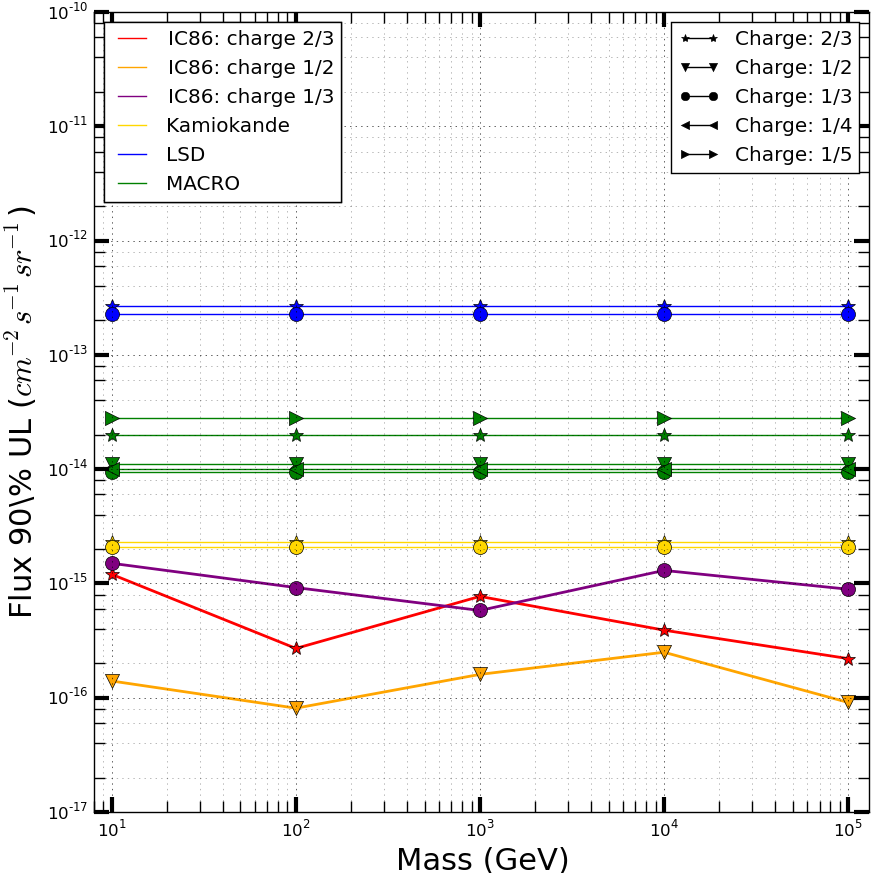
\includegraphics[width=0.6\textwidth]{chapter8/img/UpperLimitPlot_massesOBSERVED.png}
\caption{Final upper limits for SMPs with three different charges as a function of the mass. Previous experiments did not include a mass dependence and are therefore shown as straight lines.}
\label{fig:moneyplot1}
\end{figure}

\begin{figure}
\centering
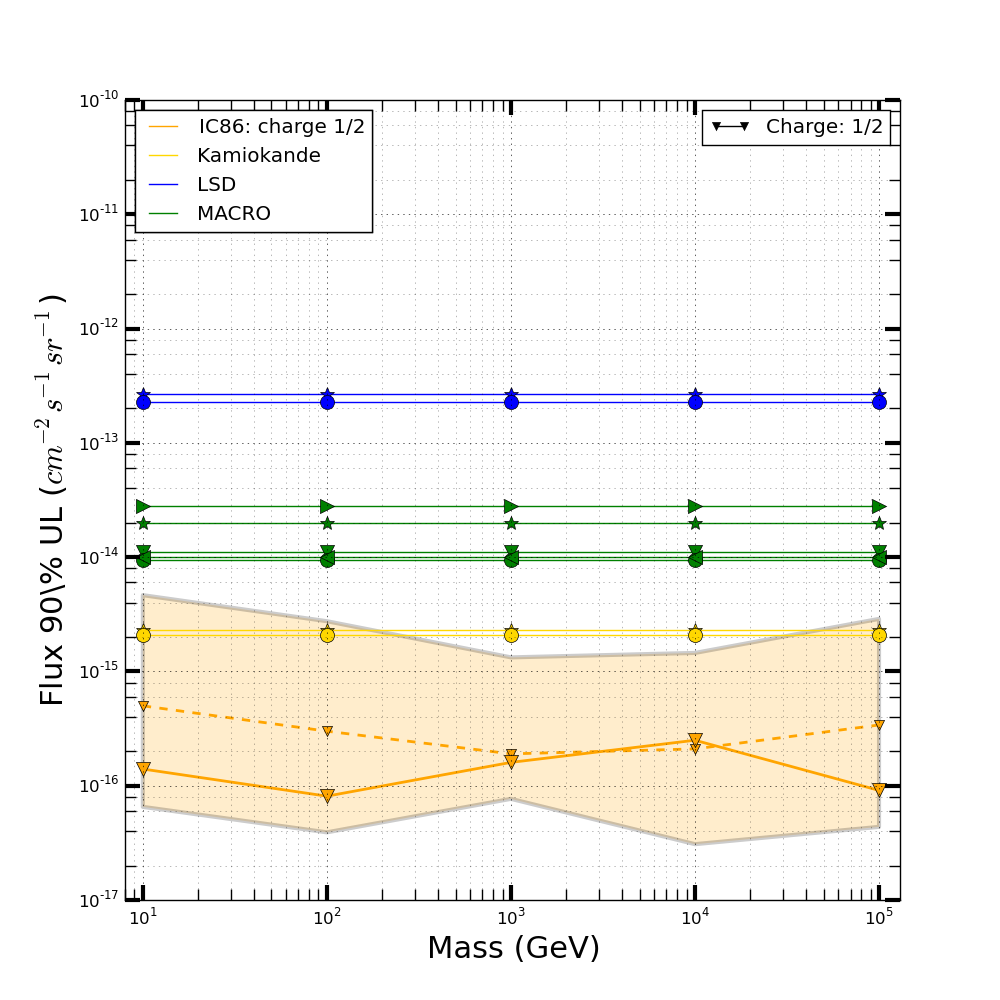
\includegraphics[width=0.6\textwidth]{chapter8/img/UpperLimitPlot_masses_withunc_0p5}
\caption{Comparison of other experiments to the upper limit obtained for SMPs with a charge 1/2 including the systematic error bands. The observed limit is shown with a solid line and the expected limit is shown with a dashed line. Other experiments did not have a mass dependence in the analysis and are therefore shown as straight lines.}
\label{fig:moneyplot2}
\end{figure}

\begin{figure}
\centering
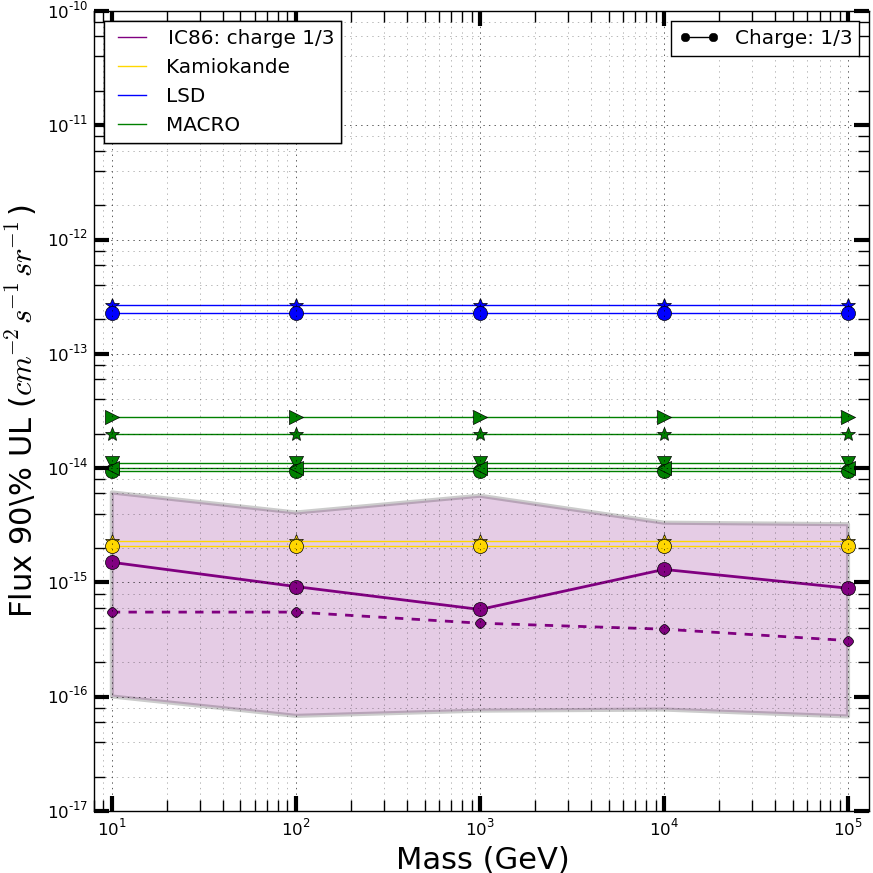
\includegraphics[width=0.6\textwidth]{chapter8/img/UpperLimitPlot_masses_withunc_0p333333333333}
\caption{Comparison of other experiments to the upper limit obtained for SMPs with charge 1/3 including the systematic error bands. The observed limit is shown with a solid line and the expected limit is shown with a dashed line. Other experiments did not have a mass dependence in the analysis and are therefore shown as straight lines.}
\label{fig:moneyplot3}
\end{figure}


\begin{figure}
\centering
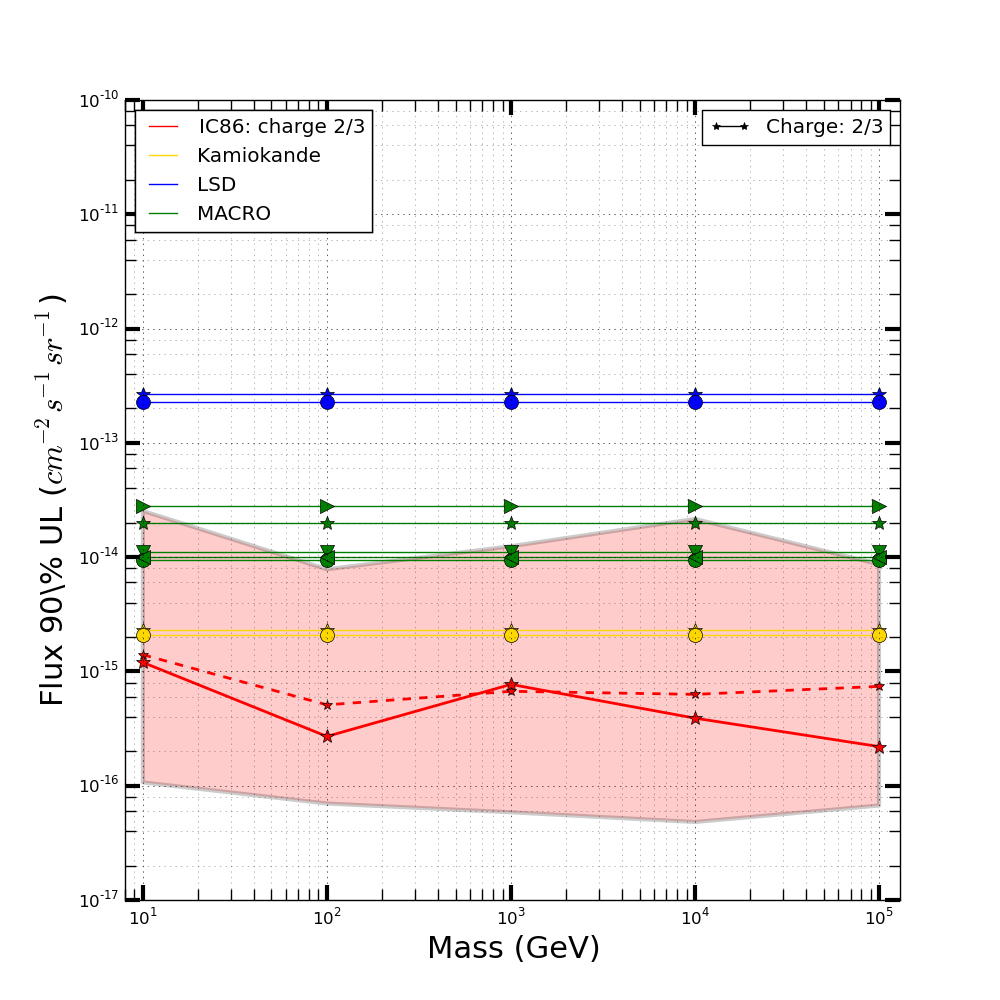
\includegraphics[width=0.6\textwidth]{chapter8/img/UpperLimitPlot_masses_withunc_0p666666666667}
\caption{Comparison of other experiments to the upper limit obtained for SMPs with charge 2/3 including the systematic error bands. The observed limit is shown with a solid line and the expected limit is shown with a dashed line. Other experiments did not have a mass dependence in the analysis and are therefore shown as straight lines.}
\label{fig:moneyplot4}
\end{figure}


